\listfiles
\documentclass[aps,
prd,
amsmath,
amssymb,
twocolumn,
%preprint,
floatfix,
groupedaddress]{revtex4-1}
%\documentclass[aps,prl,preprint,superscriptaddress]{revtex4-1}
%\documentclass[aps,prl,reprint,groupedaddress]{revtex4-1}
\usepackage[pdftex]{graphicx}% Include figure files
\usepackage{natbib}
\usepackage{lipsum}
%\usepackage{float}
%\usepackage{stfloats}
%\usepackage{fixltx2e}
\usepackage{placeins}
\usepackage{dcolumn}% Align table columns on decimal point
%\usepackage{multicol}
\usepackage{multirow}
%\usepackage{amsmath}
\usepackage{amsthm, amsfonts, amssymb}
%\usepackage{supertabular}
\usepackage{array}
\usepackage{times}
\usepackage{latexsym}
\usepackage{hyperref}
\hypersetup{backref,  
%pdfpagemode=FullScreen,  
colorlinks=true,
linkcolor=red,
filecolor=red,
citecolor=blue}
\usepackage{epsfig}
\usepackage{subfigure}
% \usepackage{multicol}
%\usepackage{acronym}
%\usepackage[caption=false]{caption}
\usepackage{bm}% bold math
\usepackage[usenames,dvipsnames]{color}
\usepackage[normalem]{ulem}
\newcommand{\Sum}{\displaystyle\sum\limits}
\newcommand{\Int}{\displaystyle\int\limits}
\newcommand{\ii}{{\rm i}}
\newcommand{\D}{\mathrm{d}}
\newcommand{\eff}{\mathrm{eff}}
\newcommand{\phys}{\mathrm{phys}}
\newcommand{\real}{\mathrm{real}}
\newcommand{\peak}{\mathrm{peak}}
\newcommand{\EOB}{\mathrm{EOB}}
\newcommand{\NR}{\mathrm{NR}}
\newcommand{\RD}{\mathrm{RD}}
\newcommand{\M}{\mathrm{M}}
\newcommand{\EFF}{\mathrm{EFF}}
\newcommand{\X}{\mathrm{X}}
\newcommand{\Y}{\mathrm{Y}}
\newcommand{\Z}{\mathrm{Z}}
\newcommand{\horizon}{\mathrm{Horizon}}
\newcommand{\opt}{\mathrm{opt}}
\newcommand{\bnk}{\mathrm{bank}}
\newcommand{\iso}{\mathrm{iso}}
\newcommand{\refr}{\mathrm{ref}}
\newcommand{\start}{\mathrm{start}}
\newcommand{\mn}{\mathrm{min}}
\newcommand{\mx}{\mathrm{max}}
\newcommand{\tr}{\mathrm{tr}}
\newcommand{\mm}{\mathrm{mm}}
\newcommand{\Hyb}{\mathrm{Hyb}}
\newcommand{\leftn}{\left|\left|}
\newcommand{\rightn}{\right|\right|}
\newcommand{\lefti}{\left\langle}
\newcommand{\righti}{\right\rangle}
\newcommand{\Mis}{\mathcal{M}}
\newcommand{\Olap}{\mathcal{O}}
\newcommand{\FF}{\mathrm{FF}}
\newcommand{\MM}{\mathrm{MM}}
\newcommand{\N}{\mathrm{N}}
\newcommand{\cyc}{\mathrm{cyc}}
\newcommand{\E}{\mathcal{E}}

\newcommand{\red}{\textcolor{red}}
\newcommand{\harald}[1]{\textcolor{RawSienna}{#1}}

\makeatletter
\newcommand{\etal}{\textit{et~al}\@ifnextchar{\relax}{.\relax}{\ifx\@let@token.\else\ifx\@let@token~.\else.\@\xspace\fi\fi}}
\makeatother

\def\l({\left(}
\def\r){\right)}


%%%%%%%%%%%%%%%%%%%%%%%%%%%%%%%%%%%%%%%%%%%%%%%%%%%%%%%%%%%%%%%%
% Affiliations
%%%%%%%%%%%%%%%%%%%%%%%%%%%%%%%%%%%%%%%%%%%%%%%%%%%%%%%%%%%%%%%%
\newcommand{\CITA}{\affiliation{Canadian Institute for Theoretical
    Astrophysics, 60 St.~George Street, University of Toronto,
    Toronto, ON M5S 3H8, Canada}} %
\newcommand{\CIFAR}{\affiliation{Canadian Institute for Advanced Research, 180 Dundas St.~West, Toronto, ON M5G 1Z8, Canada}} %
\newcommand{\DAA}{\affiliation{Department of Astronomy and Astrophysics, 50 St.\ George Street, University of Toronto, Toronto, ON M5S 3H4, Canada}}






%opening
\begin{document}
\author{}
\affiliation{}
\date{\today}
\title{Binary black hole template banks with Numerical Relativity waveforms.}
\begin{abstract}
Coalescing black hole binaries are expected to be important sources for
detection by the Advanced Laser Interferometer Gravitational-wave
Observatory (LIGO) and Advanced Virgo. With a 10-fold increase in
sensitivity from their initial incarnations, these second generation detectors will 
be able to detect such systems at distances up to a few Gpc. Current searches for
binary black holes (BBHs) use banks of waveforms, modelled using the weak-field
slow-motion post-Newtonian (PN) approximation, as filters with which to
matched-filter the detector data. \red{[HP: This sounds like {\em all} current searches use {\em exclusively} PN templates.  Please clarify wording and remove this red]} These approximate waveforms do not
model the merger phase of the binary's evolution, where strong-field
effects dominate. For massive binaries, the merger will occur in the
sensitive frequency band of LIGO. Recent advances in Numerical
Relativiy (NR) have led to high-accuracy simulations of the
late-inspiral and mergers of BBHs, with fully-numerical solutions of Einstein's field
equations. 
\red{[HP: Note that the rest of abstract is rewritten]}
This paper explores the direct use of NR waveforms for the
  construction of detection banks.  Utilizing only six already
  completed NR simulations for non-spinning BBH systems, we construct
  a template bank that covers mass-ratios $q\le 10$ and chirp-masses
  ${\cal M}_c\gtrsim 28M_\odot$.  Hybridizing these six NR waveforms
  with PN inspiral waveforms, we construct a template bank that covers
  a larger region of the non-spinning parameter space, namely $q\le
  10$ and component masses $m_1,m_2\gtrsim 12M_\odot$.  The region of
  parameter space coverable is limited by the available mass-ratios in
  NR simulations and the truncation error of the post-Newtonian
  waveforms used in the hybrids.  We estimate that 26 NR simulations
  of approximately 50 orbits in length will be needed to construct a
  NR-PN hybrid template covering the complete non-spinning parameter
  space for mass ratios $1 \leq q \leq 10$.  These template banks are
  constructed such that the combined SNR loss from the discrete
  template spacing and the modeling error due to PN truncation error
  is below 3 per cent.
 % Current literature already has simulations available for
 %    mass-ratios $(m1/m2) = \{1,2,3,4,6,8\}$, that span $15-33$
 %    inspiral orbits before merger.  We propose to use gravitational
 %    waves (GWs) extracted from these NR simulations as a detection
 %    bank for LIGO, which is possible down to a total mass between
 %    about 60$M_\odot$ and 100$M_\odot$. To cover this parameter space
 %    at lower masses, one can use hybrid gravitational waveforms, where
 %    NR waveforms have been stitched to PN waveforms, which lowers the
 %    minimum mass to a component mass of about $m_2 = 12M_\odot$. At
 %    lower masses than this, the error between consecutive mass ratios
 %    becomes large, and more NR simulations are necessary. In addition,
 %    the errors within the hybrid waveforms themselves become large due
 %    to unknown higher-order terms in the PN waveforms. We find that we
 %    are able to completely cover the non-spinning parameter space for
 %    mass ratios $1 \leq q \leq 10$ with 26 NR simulations of
 %    approximately 50 orbits in length.
\end{abstract}
\maketitle
\section{Introduction}
% $Id$

In chapter \ref{c:findchirp} we describe in detail the algorithms used to
inspiral signals from binary neutron starts and binary black hole MACHOs in
the LIGO data.  findchirp. We first carefully define the conventions that we
use for analysis quantities in section \ref{s:conventions}; in particular the
definition of the Fourier transform and the power spectral density. Section
\ref{s:waveforms} gives a brief description of the the waveforms used and
section \ref{s:matchedfilter} describes the implementation of the matched
filter.  Spurious noise may cause the output of the matched filter to be large
and so in section \ref{s:chisq} we describe our implementation of the $\chi^2$
time--frequency discriminator proposed in~\cite{allen}. Section
\ref{s:practical} contains additional details of the search particular to our
implementation: the computation of the inverse power spectrum and the trigger
selection algorithm. This is followed by a brief conclusion which summarized
the methods used and outlines some future directions for improvement.

\section{Fourier Transform Conventions}
\label{s:ftconv}

There are two possible sign conventions for the Fourier transform of a time
domain quantity $v(t)$. In this thesis, we define the Fourier transform
$\tilde{v}(f)$ of a $v(t)$ to be
\begin{equation}
\label{eq:ft}
\tilde{v}(f)=\int_{-\infty}^\infty dt\,v(t)\, e^{- 2 \pi i f t}
\end{equation}
and the inverse Fourier transform to be 
\begin{equation}
\label{eq:ift}
v(t)=\int_{-\infty}^\infty df\,\tilde{v}(f)\, e^{2 \pi i f t}.
\end{equation}
This convention differs from that used in some gravitational wave literature,
but is the adopted convention in the LIGO Scientific Collaboration.


\section{Methodology}\label{s1:methodology}

\subsection{post-Newtonian waveforms}\label{s2:PNwaveforms}


Post-Newtonian (PN) theory is a perturbative approach to describing the
motion of a compact object binary, during the slow-motion and weak-field 
regime, i.e. the inspiral phase. The conserved energy of a binary in orbit,
$E$, has been calculated to 3PN order in literature~\citep{Jaranowski:1997ky,
Jaranowski:1999ye,Jaranowski:1999qd,Damour:2001bu,Blanchet:2003gy,
Damour:2000ni,Blanchet:2002mb}.
Using the adiabatic approximation, we treat the course of inspiral as a series
of radially shrinking circular orbits. This is valid during the inspiral when
the angular velocity of the binary evolves more slowly than the orbital 
time-scale. The radial separation shrinks as the binary loses energy to 
gravitational radiation that propagates outwards from the system. 
% For a binary with individual component masses $m_1$ and $m_2$ and total mass
%$M=m_1+m_2$, the conserved energy accurate to 3PN
% can be written as \citep{Jaranowski:1997ky,Jaranowski:1999ye,Jaranowski:1999qd,Damour:2001bu,Blanchet:2003gy,Damour:2000ni,Blanchet:2002mb}
% \begin{equation}
% \begin{split}\label{eq:E3PN}
% E_3(v)=&-\dfrac{1}{2}\eta v^2 \left[1- \l(\dfrac{3}{4}+\dfrac{1}{12}\eta\r)v^2 - \l(\dfrac{27}{8}-\dfrac{19}{8}\eta\right.\right.\\
% +&\left.\left.\dfrac{1}{24}\eta^2 \r)v^4 - \l(\dfrac{675}{64}-\l(\dfrac{34445}{576}-\dfrac{205}{96}\pi^2\r)\eta\right.\right.\\
% +&\left.\left.\dfrac{155}{96}\eta^2 +\dfrac{35}{5184}\eta^3\r) v^6\right],
% \end{split}
% \end{equation}
% where $\eta=m_1m_2/(m_1+m_2)^2$, $v=(\pi Mf)^{1/3}$ is the characteristic velocity of the binary, and $f$ denotes the frequency of the emitted gravitational wave throughout.
The energy flux from a binary $F$ is known in PN theory to 3.5PN 
order~\cite{FluxandE3-5PN,Blanchet:2004ek,Blanchet:2005tk,Blanchet:2004bb}.
% \begin{equation}
% \begin{split}\label{eq:Ft3.5PN}
% F_{3.5}(v)=&\dfrac{32}{5}\eta^2 v^{10}\left[1 - \l(\dfrac{1247}{336}+\dfrac{35}{12}\eta\r)v^2+4\pi v^3\right.\\
% -&\left.\l(\dfrac{44711}{9072}-\dfrac{9271}{504}\eta -\dfrac{65}{18}\eta^2 \r)v^4\right.\\
% -&\left.\l(\dfrac{8191}{672}+\dfrac{583}{24}\eta\r)\pi v^5+ \l(\dfrac{6643739519}{69854400}\right.\right.\\
% +&\left.\left.\dfrac{16}{3}\pi^2 -\dfrac{1712}{105}\gamma +\l(\dfrac{41}{48}\pi^2 -\dfrac{134543}{7776}\r)\eta \right.\right.\\
% -&\left.\left.\dfrac{94403}{3024}\eta^2 -\dfrac{775}{324}\eta^3 -\dfrac{856}{105}\textrm{log}(16v^2)\r)v^6\right.\\ 
% -&\left.\l(\dfrac{16285}{504}-\dfrac{214745}{1728}\eta -\dfrac{193385}{3024}\eta^2 \r)\pi v^7\right],
% \end{split}
% \end{equation}
% where $\gamma$ is Euler's constant. In the limit $\dot{\omega}/\omega \ll 1$, 
% we can approximate the energy of the system to be the energy averaged over a 
% period. 
Combining the energy balance equation, $\D E/\D t = -F$, with Kepler's law 
gives a description of the radial and orbital phase evolution of the binary. 
We start the waveform where the GW frequency enters the sensitive frequency 
band of advanced LIGO, i.e. at $15$Hz. 
% \begin{subequations}\label{eq:PNOrbitalEvolution01}
% \begin{align}
% \dfrac{\D\phi}{\D t} - \dfrac{v^3}{M} &= 0,\label{eq:PNOrbitalEvolution01_01}\\
% \dfrac{\D v}{\D t} + \dfrac{F(v)}{M\l(\D E/\D v\r)} &= 0.\label{eq:PNOrbitalEvolution01_02}
% \end{align}
% \end{subequations}
Depending on the way the expressions for orbital energy and flux
%in Eq.~\ref{eq:E3PN} \& \ref{eq:Ft3.5PN} 
are combined to obtain the coordinate evolution for the binary,
%to solve Eq.~\ref{eq:PNOrbitalEvolution01}, 
we get different Taylor\{T1,T2,T3,T4\} time-domain approximants. Using the 
stationary phase approximation~\cite{MatthewsWalker}, frequency-domain 
equivalents of these approximants, i.e. TaylorF$n$, can be constructed. 
Past GW searches have extensively used the TaylorF2 approximant, as it has a
closed form and mitigates the computational cost of generating and numerically
fourier-transforming time-domain template~\cite{Colaboration:2011nz,Abadie:2010yb,
Abbott:2009qj,Abbott:2009tt,Messaritaki:2005wv}.
We refer the reader to Ref.~\cite{PNtheoryLivingReviewBlanchet,JolienGWPhysAst}
for an overview.
From the coordinate evolution, we obtain the emitted gravitational waveform;
approximating it by the quadrupolar multipole $h_{2,\pm 2}$ which is the 
dominant mode of the waveform.
% in previous waveform-related studies~\cite{CompTemplates2001,CompTemplates2009,
% Miller:2005qu,NRPNComparisonBoyleetal,NRPNComparisonBaker2007,Boyle:2011dy,
% MacDonald:2011ne,Brown:2012nn}.



\subsection{Effective-One-Body waveforms}\label{s2:EOBwaveforms}


Full numerical simulations are available for a limited number of binary 
mass combinations. We use a recently proposed EOB 
model~\cite{BuonannoEOBv2Main}, which we refer to as EOBNRv2, as a substitute
to model the signal from binaries with arbitrary component masses
in this paper. This model was calibrated to most of the numerical simulations
that we use to construct templates banks, which span the range of masses 
we consider here well. So we expect this approximation to hold. We describe the
model briefly here.

The EOB formalism maps the dynamics of a two-body system onto an effective-mass
moving in a deformed Schwarzschild-like background~\citep{EOBOriginalBuonannoDamour}.
The formalism has evolved to use Pad\'{e}-resummations of perturbative 
expansions calculated from PN theory, and allows for the introduction of higher
(unknown) order PN terms that are subsequently calibrated against NR 
simulations of BBHs 
\cite{EOBdevel01,EOBdevel02,EOBNRdevel03,DamourFluxhlm01,EOBNRdevel01}. The EOB 
model proposed recently in Ref.~\citep{BuonannoEOBv2Main} has been calibrated 
to SpEC NR waveforms for binaries of mass-ratios $q=\{1,2,3,4,6\}$, where 
$q\,\equiv \, m_1/m_2$, and is the one that we use in this paper (we will refer
to this model as EOBNRv2).

The dynamics of the binary enters in the metric coefficient of the deformed
Schwarzschild-like background, the EOB Hamiltonian \cite{EOBOriginalBuonannoDamour}, 
and the radiation-reaction force. 
% In polar coordinates $(r,\Phi)$, the EOB 
% metric is written as
% \begin{equation}\label{eq:dsEOB}
% \D s_{\eff}^2 = -A(r)\D t^2 + \dfrac{A(r)}{D(r)}\D r^2 + r^2\left(\D\Theta^2 + \sin^2\Theta \D\Phi^2\right).
% \end{equation}
These
%metric coefficients $A(r)$ and $D(r)$ 
are known to 3PN order \cite{EOBOriginalBuonannoDamour,PadeAD} from PN theory.
The 4PN \& 5PN terms were introduced in the potential $A(r)$, which was 
Pad\'{e} resummed and calibrated to NR simulations
\citep{EOBNRdevel01,EOBNRdevel02,EOBNRdevel03,EOBNRdevel04,BuonannoEOBv2Main}.
We use the resummed potential calibrated in Ref.~\cite{BuonannoEOBv2Main} 
(see Eq.~(5-9)). The geodesic dynamics of the reduced mass 
$\mu\,=\,m_1 m_2 / M$ in the deformed background 
%of Eq.~\eqref{eq:dsEOB} 
is described by
the Hamiltonian $H^{\eff}$ given by Eq.~(3) in \cite{BuonannoEOBv2Main}.
% , which can be written as \cite{EOBOriginalBuonannoDamour,PadeAD}
% \begin{equation}
% \begin{split}
% H^{\eff} =\, & \mu\hat{H}^{\eff} \\
%          =\, & \mu\sqrt{A(r) \left( 1 +  \dfrac{A(r)}{D(r)}p_r^2 + 2(4 - 3\eta)\eta \dfrac{p_r^4}{r^2} + \dfrac{p^2_{\Phi}}{r^2} \right)},
% \end{split}
% \end{equation}
% where $(p_r,p_{\Phi})$ are momenta conjugate to the $(r,\Phi)$ coordinates. 
The Hamiltonian describing the conservative dynamics of the binary
(labeled the \textit{real} Hamiltonian $H^{\real}$) is related to 
$\hat{H}^{\eff}$ as in Eq.~(4) of \cite{BuonannoEOBv2Main}.
% \begin{equation}
% H^{\real} = \mu\hat{H}^{\real} = M \sqrt{1 + 2\eta (\hat{H}^{\eff} - 1)}.
% \end{equation}
The inspiral-merger dynamics can be obtained by numerically solving the 
Hamiltonian equations of motion for $H^{\real}$, see e.g. Eq.(10)
of~\cite{BuonannoEOBv2Main}. 

The angular momentum carried away from the binary
by the outwards propagating GWs results in a radiation-reaction force
%$\hat{F}_{\Phi}$ 
that causes the orbits to shrink.
% ,
% \begin{eqnarray}
%\dfrac{\D r}{\D\hat{t}} &\equiv & \dfrac{\partial \hat{H}^{\real}}{\partial p_r} = \dfrac{A(r)}{\sqrt{D(r)}}\dfrac{\partial \hat{H}^{\real}}{\partial p_{r*}} (r, p_{r*}, p_{\Phi}) ,\\
%\dfrac{\D\Phi}{\D\hat{t}} &\equiv & \hat{\Omega} = \dfrac{\partial \hat{H}^{\real}}{\partial p_{\Phi}} (r, p_{r*}, p_{\Phi}) , \\ 
%\dfrac{\D p_{r_*}}{\D\hat{t}} &=& -\dfrac{A(r)}{\sqrt{D(r)}} \dfrac{\partial \hat{H}^{\real}}{\partial r} (r, p_{r*}, p_{\Phi}) ,\\
% \dfrac{\D p_{\Phi}}{\D\hat{t}} &=& \hat{F}_{\Phi},%(r, p_{r*}, p_{\Phi}) ;
% \end{eqnarray}
% where, $\hat{t}\equiv t/M$ is time in dimensionless units; and
% \begin{equation}
%\hat{F}_{\Phi} = -\dfrac{1}{\eta \hat{\Omega}} \dfrac{\D E}{\D t} = -\dfrac{1}{\eta v^3} \dfrac{\D E}{\D t},
% \hat{F}_{\Phi} = -\dfrac{1}{\eta v^3} \dfrac{\D E}{\D t},
% \end{equation}
% where, $v=\hat{\Omega}^{1/3}=(\pi Mf)^{1/3}$ as before, and $f$ is the 
% instantaneous frequency of the emitted GWs. 
This is due to the flux of energy from the binary, which
%flux $\D E/\D t$ 
is obtained by summing over the contribution from each term in the multipolar
decomposition of the inspiral-merger EOB waveform.
% , i.e.
% \begin{equation}\label{eq:definedEdt}
% \frac{\D E}{\D t} = \frac{\hat{\Omega}^2}{8\pi} \Sum_{l}\Sum_{m} \left|\frac{\mathcal{R}}{M} h_{lm}\right|^2,
% \end{equation}
% where $\mathcal{R}$ is the physical distance to the binary, and 
%$h_{lm}$, which are 
% the EOB waveform multipoles, 
%defined implicitly as
%  \begin{equation}\label{eq:hlmdef}
%  h_+ - \ii h_{\times} = \dfrac{M}{\mathcal{R}} \Sum^{\infty}_{l=2} \Sum^{m=l}_{m = -l} Y^{lm}_{-2}\, h_{lm},
%  \end{equation}
%  where $Y^{lm}_{-2}$ are spin $-2$ weighted spherical harmonics, 
%  and $h_{+,\times}$ are the two orthogonal polarizations of the incoming GW. 
% These multipoles 
% %$h_{lm}$ 
% are functions of the orbital phase of the binary $\propto e^{-\ii m\Phi}$.
Complete resummed expressions for these multipoles~\cite{DamourFluxhlm01} can be 
read off from Eq.(13)-(20) of Ref.~\cite{BuonannoEOBv2Main}. In this paper, 
as for PN waveforms, we model the inspiral-merger part 
%$l=2\ldots 8$ to compute the energy flux, and approximate the 
%summation in Eq.~\ref{eq:hlmdef} 
by summing over the dominant $h_{2,\pm 2}$ multipoles.

The EOB merger-ringdown part is modeled as a sum of $N$ quasi-normal-modes 
(QNMs),
% \begin{equation}
% h_{lm}^{\RD}(t) = \Sum^{N-1}_{n=0}A_{lmn}e^{-\ii\sigma_{lmn}(t-t_{lm}^{\mathrm{match}})},
% \end{equation}
where $N=8$ for EOBNRv2~\citep{EOBNRdevel01,EOBNRdevel02,EOBNRdevel04,BHRDQNMs}.
The ringdown frequencies depend on the mass and spin of the BH that is formed 
from the coalescence of the binary. The inspiral-merger and ringdown parts are
attached by matching them at the time at which the amplitude of the 
inspiral-merger waveform peaks.
%, i.e. at $t_{lm}^{\mathrm{match}}=t^{lm}_{\peak}$
~\citep{EOBNRdevel01,BuonannoEOBv2Main}. The matching procedure followed
% involves equating the complex amplitude and
% phase (and its derivative) of $h_{lm}(t)$ and $h_{lm}^{\RD}(t)$ over a small 
% interval of time ending at $t_{lm}^{\mathrm{match}}$, from which we obtain the
% complex amplitudes $A_{lmn}$. 
is explained in detail Sec.~II~C of Ref.~\citep{BuonannoEOBv2Main}.
%gives further details of this procedure. 
By combining them, we obtain the complete waveform for a BBH system.
% We combine the inspiral-merger waveform $h_{lm}(t)$ and the ringdown 
% waveform $h^{\RD}(t)$ to obtain the complete inspiral-merger-ringdown EOB 
% waveform $h^{\textrm{IMR}}(t)$, i.e.
% \begin{equation}
% h^{\textrm{IMR}}_{lm}(t) = h_{lm}(t)\Theta(t^{\mathrm{match}}_{lm}-t) + h^{\RD}(t)\Theta(t-t^{\mathrm{match}}_{lm}),
% \end{equation}
% where $\Theta(x)=1$ for $x\geq 0$, and 0 otherwise. These multipoles are then
% combined to give the two orthogonal polarizations of the gravitational 
% waveform, $h_+$ and $h_{\times}$, as in Eq.~\ref{eq:hlmdef}.



%%%%%%%%%%%%%%%%%%%%%%%%%%%%%%%%%%%%%%%%%%%%%%%%%%%%%%%%%%%%%%%%
\subsection{Numerical Relativity Waveforms}\label{s2:NRwaveforms}

The numerical relativity waveforms used in this paper were produced
with the SpEC code~\cite{spec}, a multi-domain pseudospectral code to solve
Einstein's equations. SpEC uses Generalized Harmonic coordinates,
spectral methods, and a flexible domain decomposition, all of which
contribute to it being one of the most accurate and efficient codes
for computing the gravitational waves from binary black hole
systems. High accuracy numerical simulations of the late-inspiral,
merger and ringdown  of coalescing binary black-holes have been
recently performed for mass-ratios $q\equiv m_1/m_2\in\{1,2,3,4,6,8\}$
~\cite{Buchman:2012dw,Scheel:2008rj,NRPNComparisonBoyleetal,Mroue:2012kv}.

The equal-mass,
non-spinning waveform covers 33 inspiral orbits and was first discussed
in~\cite{MacDonald:2012mp,Mroue:2012kv}. 
This waveform was obtained with numerical techniques similar to those 
of~\cite{Buchman:2012dw}. The unequal-mass waveforms of mass ratios 
$2, 3, 4,$ and $6$ were presented in detail in Ref.~\cite{Buchman:2012dw}.
The simulation with mass ratio $6$ covers about 20 orbits and the
simulations with mass ratios 2, 3, and 4 are somewhat shorter and
cover about 15 orbits. The unequal mass waveform with mass ratio 8 was
presented as part of the large waveform catalog
in~\cite{Mroue:2013xna,Mroue:2012kv}. It is approximately 25 orbits in
length. 
% As it becomes possible to simulate BBH evolution for longer times, in our 
% template bank construction we assume that simulations that span $\gtrsim 20$
% orbits, including the inspiral, merger and ringdown cycles, are (will be) 
% available by the time Advanced LIGO begins observation runs. 
We summarize the NR simulations used in this study in 
Table~\ref{table:etalist4}. In the table, we also give the  
lowest total masses for which the NR waveforms span the aLIGO 
band, starting at $15$~Hz.

\begin{table}
\begin{tabular}{| c | c | c | c |}
\hline
$\hspace{10pt}\eta\hspace{10pt}$ & \hspace{15pt} q\hspace{15pt} & Length (in orbits) & Minimum total mass ($M_\odot$)\\ \hline
0.25 & 1 & 33 & 49 \\
0.2222 & 2 & 15 & 76 \\
0.1875 & 3 & 18 & 82 \\
0.1600 & 4 & 15 & 87 \\
0.1224 & 6 & 20 & 83 \\
0.0988 & 8 & 25 & 83 \\
%0.0884 & 9.2 & ?? \\
\hline
\end{tabular}
\caption{SpEC BBH simulations used in this study.  Given are symmetric mass-ratio $\eta$, mass-ratio $q=m_1/m_2$, and the length in orbits of the simulation. 
The last column gives the lowest total masses for which the NR simulations 
cover the entire coalescence process within the sensitive band of aLIGO,
starting at $15$~Hz.}
\label{table:etalist4}
\end{table}



%%%%%%%%%%%%%%%%%%%%%%%%%%%%%%%%%%%%%%%%%%%%%%%%%%%%%%%%%%%%%%%%
\subsection{Hybridization procedures}\label{s2:NRpNhybridwaveforms}
The hybridization procedure used for this investigation is described in Sec.~3.3 of Ref.~\cite{MacDonald:2011ne}: The PN waveform, $h_\text{PN}(t)$, is time and phase shifted to match the NR waveform, $h_\text{NR}(t)$, and they are smoothly joined together in a GW frequency interval centered at $\omega_m$ with width $\delta\omega$: 
\begin{equation}\label{eq:omega_match}
\omega_m-\frac{\delta\omega}{2} \le \omega \le \omega_m+\frac{\delta\omega}{2}.
\end{equation}
This translates into a matching interval $t_{\rm min}<t<t_{\rm max}$ because the GW frequency continuously increases during the inspiral of the binary. As argued in Ref.~\cite{MacDonald:2011ne}, we
choose $\delta\omega = 0.1\omega_m$ because it offers a good compromise of suppressing residual oscillations in the matching time, while still allowing $h_\text{PN}(t)$ to be matched as closely as possible to the beginning of $h_\text{NR}(t)$.

The PN waveform depends on a (formal) coalescence time, $t_c$, and phase, $\Phi_c$. These two parameters are determined by minimizing the GW phase difference in the matching interval $[t_\text{min}, t_\text{max}]$ as follows:
\begin{equation}\label{eq:tcphic_bymin}
t_c', \Phi_c' = \mathrm{ \mathop{arg min}_{t_c, \Phi_c}}\int^{t_{\rm max}}_{t_{\rm min}} \big(
  \phi_{\rm PN}(t;t_c,\Phi_c) - \phi_{\rm NR} (t) \big)^2 \rm{d}t,
\end{equation}
where $t_c'$ and $\Phi_c'$ are the time and phase parameters for the best matching between $h_\text{PN}(t)$ and $h_\text{NR}(t)$, and $\phi(t)$ is the phase of the (2,2) mode of the gravitational
radiation. Since we consider only the (2,2) mode, this procedure is identical to time and phase shifting the PN waveform until it has best agreement with NR as measured by the integral in Eq.~(\ref{eq:tcphic_bymin}). The hybrid waveform is then constructed in the form
\begin{equation}
h_\text{H}(t) \equiv \mathcal{F}(t) h_\text{PN}(t;t'_c,\Phi'_c) + \big[1- \mathcal{F}(t)\big]  h_\text{NR} (t), 
\end{equation}
where $\mathcal{F}(t)$ is a blending function defined as
\begin{eqnarray}
\mathcal{F}(t) \equiv 
\left\{
\begin{array}{ll}
  1, &  t < t_{\rm min} \\ 
 \cos^2\frac{\pi(t - t_{\rm min})}{2(t_{\rm max} - t_{\rm min})},\quad\quad &  t_{\rm min}
  \leq t < t_{\rm max} \\ 
  0. & t\geq t_{\rm max}  .
\end{array}
\right.\label{eq:BlendingFunction}
\end{eqnarray}
In this work, we construct all hybrids using the same procedure, Eqs.~(\ref{eq:omega_match})--(\ref{eq:BlendingFunction}), and vary only the PN approximant and the matching frequency $\omega_m$.


\subsection{Quantifying waveform accuracy \& bank
  effectualness}\label{s2:quantifyingerrors} 
%%%%%%%%%%%%%%%%%%%%%%%%%%%%%%%%%%%%%%%%%%%%%%%%%%%%%%%%%%%%%%%%%%%%%%%%%%%%%%%

To assess the recovery of SNR from template banks with NR waveforms or NR-PN 
hybrids as templates, we use the measures proposed in
Ref.~\cite{FittingFactorApostolatos,Sathyaprakash:1991mt,Balasubramanian:1995bm}. 
The gravitational waveform emitted during and driving a BBH coalescence is
denoted as $h(t)$, or simply $h$. The inner product between two 
waveforms $h_1$ and $h_2$ is
\begin{equation}\label{eq:overlap}
(h_1|h_2) \equiv 
4\int^{f_\mathrm{Ny}}_{f_\mathrm{min}}\dfrac{\tilde{h}_1(f)\tilde{h}_2^*(f)}{S_n(f)}\D f,
\end{equation}
where $S_n(f)$ is the one-sided power spectral density (PSD) of the detector
noise, which is assumed to be stationary and Gaussian with zero mean; 
$f_\mathrm{min}$ is the lower frequency cutoff for filtering; $f_\mathrm{Ny}$
is the Nyqyuist frequency corresponding to the waveform sampling rate; and 
$\tilde{h}(f)$ denotes the Fourier transform of $h(t)$.
% The noise PSD $S_n(f)$ is defined by
% \begin{equation}
%  \langle\tilde{n}(f)\tilde{n}^*(f')\rangle = \dfrac{1}{2}S_n(f)\delta(f-f'),
% \end{equation}
% where $\tilde{n}(f)$ is the Fourier transform of the detector noise $n(t)$, and
% $\langle\dots \rangle$ denotes an average over an ensemble of noise 
% realizations. 
In this paper, we take $S_n(|f|)$ to be the \textit{zero-detuning high power} 
noise curve for aLIGO, for both bank placement and overlap
calculations~\cite{aLIGONoiseCurve}; and set the lower frequency cutoff 
$f_\mathrm{min} =15$~Hz. The peak GW frequency for the lowest binary masses
that we consider, i.e. for $m_1+m_2\simeq 12M_\odot$, is $\sim 2.1$~kHz during
the ringdown phase. We sample the waveforms at $8192$~Hz, preserving the 
information content up to the Nyquist frequency $f_\mathrm{Ny}=4096$~Hz.
% The normalized overlap between the two waveforms,
% \begin{equation}
% (\hat{h}_1|\hat{h}_2) = \dfrac{(h_1|h_2)}{\sqrt{(h_1|h_1)(h_2|h_2)}},
% \end{equation}
% is also sensitive to a relative constant phase and time offset between $h_1$ 
% and $h_2$, $\phi_c$ and $t_c$, apart from the intrinsic mass parameters. These
A waveform, h, is normalized (made to be a unit vector) by 
$\hat{h} = h/\sqrt{h | h}$. In addition to being senstive to their 
intrinsic mass parameters, the inner product of two normalized waveforms is 
sensitive to phase and time shift differences between the two, $\phi_{c}$ and
$t_{c}$.  These two parameters ($\phi_c$ and $t_c$) can be analytically
maximized over to obtain the maximized overlap $\Olap$,
\begin{equation}\label{eq:maxnormolap}
\Olap(h_1,h_2) = 
\underset{\phi_c,t_c}{\mathrm{max}}\,\l(\hat{h}_1|\hat{h}_2(\phi_c,t_c)\r),
\end{equation}
which gives a measure of how ``close'' the two waveforms are in the waveform
manifold, disregarding differences in overall amplitude. The \textit{mismatch}
$\mathcal{M}$ between the two waveforms is then
\begin{equation}\label{eq:mismatch}
\mathcal{M}(h_1,h_2) = 1 - \Olap(h_1,h_2).
\end{equation}

Matched-filtering detection searches employ a discrete bank of modeled
waveforms as filters. The optimal signal-to-noise ratio (SNR) is obtained when
the detector strain $s(t)\equiv h^{\tr}(t) + n(t)$ is filtered with the 
\textit{true} waveform $h^{\tr}$ itself, i.e.
\begin{equation}
 \rho_{\mathrm{opt}} = \underset{\phi_c,t_c}{\mathrm{max}}\,\l(h^{\tr}|\hat{h}^{\tr}(\phi_c,t_c)\r) = \leftn h^{\tr}\rightn,
\end{equation}
where $\leftn h^{\tr}\rightn\equiv\sqrt{\left(h^{\tr},h^{\tr}\right)}$ is the
noise weighted norm of the waveform. With a discrete bank of filter templates, 
the SNR we recover
\begin{equation}\label{eq:realoptimalSNR}
 \rho\simeq \Olap(h^{\tr},h_b)\leftn h^{\tr}\rightn = \Olap(h^{\tr},h_b)\,\rho_{\mathrm{opt}},
\end{equation}
where $h_b$ is the filter template in the $b$ank (subscript $b$) that has the
highest overlap with the signal $h^{\tr}$.
The furthest distance to which GW signals can be detected is proportional to 
the matched-filter SNR that the search algorithm finds the signal with. 
Note that $0\leq\Olap(h^{\tr},h_b)\leq 1$, so the recovered SNR
$\rho\leq \rho_{\mathrm{opt}}$ (c.f. Eq.~(\ref{eq:realoptimalSNR})). 
For a BBH population uniformly distributed in spacial volume, the 
detection rate would decrease as $\Olap(h^{\tr},h_b)^3$. Searches that aim at
restricting the loss in the detection rate strictly below 
$10\%\,(\mathrm{or}\, 15\%)$, would require a bank of template waveforms that
have $\Olap$ above $0.965\,(\mathrm{or}\, 0.947)$ with \textit{any} incoming
signal~\citep{WaveformAccuracy2008,WaveformAccuracy2010}.


Any template bank has two sources for loss in SNR: 
(i) the discreteness of the bank grid in the physical parameter space of the 
BBHs, and, (ii) the disagreement between the actual GW signal $h^{\tr}$ and the 
modeled template waveforms used as filters. We de-coupled these to estimate
the SNR loss. Signal waveforms are denoted as $h^\tr_x$ in what follows, 
where the superscript $\tr$ indicates a $tr$ue signal, and the subscript
$x$ indicates the mass parameters of the corresponding binary. Template
waveforms are denoted as $h^\M_b$, where $\M$ denotes the waveform $m$odel, and
$b$ indicates that it is a member of the discrete \textit{b}ank.
% To put a bound on the 
% loss in SNR due to the first, we compute the \textit{minimal match} $\MM$ of 
% the bank,
% \begin{equation}
% \MM_{\mathcal{B}} = \underset{a}{\textrm{min}}\,\underset{g\, \in\, 
% \mathrm{bank}}{\textrm{max}}\,\Olap(h^{\M}_a,h^{\M}_g),
% \end{equation}
% \red{[Harald:  Define ``a'' in this equation and for use below]}
% which gives the highest fractional loss in SNR over the entire region of 
% physical parameters $\mathcal{B}$ that the bank covers. As both the signal 
% and the template 
% are modeled with the same approximant, $\MM$ measures the loss due to the 
% discreteness of the bank grid alone. The combined fractional SNR loss at any
% point $a$ in the parameter space can be measured by computing the 
% \textit{fitting factor} $\FF$ of the bank~\cite{FittingFactorApostolatos},
% \begin{equation}\label{eq:defFF}
% \FF_{\M}(a) = \underset{g\, \in\, 
% \mathrm{bank}}{\textrm{max}}\,\Olap(h^{\tr}_a,h^{\M}_g).
% \end{equation}
% which measures the same in a small neighborhood of $a$. A detection
% search that aims at strictly less than $10\%\,(15\%)$ loss in the observable  volume of the universe (module the effect of the cosmological redshift),
% requires a bank of template waveforms that has $\FF$ above $0.965\,
% (0.947)$~\citep{WaveformAccuracy2008,WaveformAccuracy2010,CompTemplates2009}
% over the entire parameter space.
\begin{figure}
 \centering
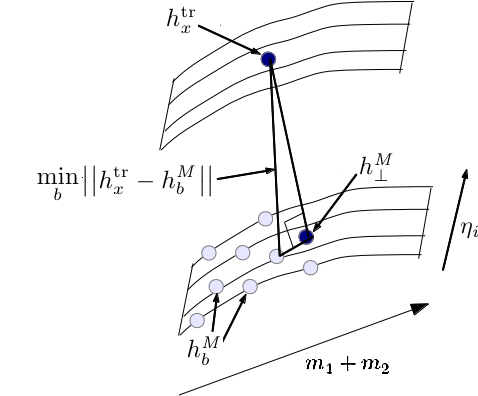
\includegraphics[width=\columnwidth]{Eff1v2.png}%\quad
\caption{We show the \textit{true} (upper) and the \textit{hybrid} (lower) 
waveform manifolds here, with the signal residing in the former, and a discrete
bank of templates placed along lines of constant mass-ratio in the latter. 
Both manifolds are embedded in the same space of all possible waveforms.
The true signal waveform is denoted as $h^{\tr}_x$, while the templates in the
bank are labelled $h^{\M}_b$. The hybrid waveform that matches the signal $H^{\tr}_x$
best is shown as $h^{\M}_\perp$. Also shown is the ``distance'' between
the signal and the hybrid template that has the highest overlap with it.
This figure is qualitatively similar to Fig.~3 of
Ref.~\cite{WaveformAccuracy2008}.}
\label{fig:EFFdiag1}
\end{figure}
% \begin{figure}
%  \centering
% 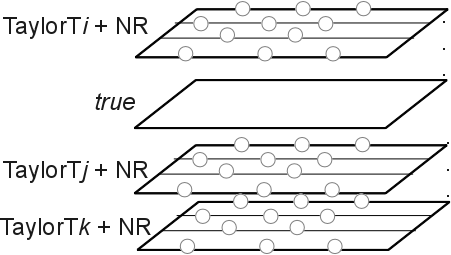
\includegraphics[width=0.8\columnwidth]{Eff2.png}%\quad
% \caption{We show the \textit{true} and the \textit{hybrid} waveform manifolds 
% relative to it. We assume that the hybrid waveform manifolds envelope 
% \textit{true} one, and so the shortest distance between a point on the true 
% manifold and any hybrid manifold would be lesser than the same between the two 
% mutually farthest hybrid manifolds; as for Eq.~(\ref{eq:hybridMMTn}).}
% \label{fig:EFFdiag2}
% \end{figure}
Fig.~\ref{fig:EFFdiag1} shows the signal $h^\tr_x$ in its manifold, and the
bank of templates $h^\M_b$ residing in the model waveform manifold, both being
embedded in the same space of all possible waveforms. The 
point $h^\M_\perp$ is the waveform which has the smallest mismatch
in the entire (continuous) model manifold with $h^\tr_x$, i.e.
$h^\M_\perp :\mathcal{M}(h^\tr_x,h^\M_\perp) = \underset{y}{\mn}\,\,\mathcal{M}(h^\tr_x,h^\M_y)$.
The fraction of the optimal SNR recovered at different points $x$ in the
binary mass space can be quantified by measuring the fitting factor $\FF$ of
the bank~\cite{FittingFactorApostolatos},
\begin{equation}\label{eq:ffmismatch}
 \FF(x) = 1 - \underset{b}{\mn}\,\,\mathcal{M}(h^\tr_x, h^\M_b).
\end{equation}
For two waveforms $h_1$ and $h_2$ close to each other in the
waveform manifold: $\leftn h_1\rightn \simeq\leftn h_2\rightn$, and mutually
aligned in phase and time such that the overlap between them is maximized, 
\begin{equation}
%  \begin{align}
  \leftn h_1 - h_2\rightn^2 \simeq 2\l( h_1 |h_1\r)\left(1 - \dfrac{\l( h_1 |h_2\r)}{\sqrt{\l( h_1 |h_1\r)}\sqrt{\l( h_1 |h_1\r)}}\right).
%  &= 2\leftn h_1\rightn^2 \Mis\left(h_1,h_2\right)
% \end{align}
\end{equation}
The mismatch can, hence, be written as 
(c.f. Eq.~(\ref{eq:mismatch}))
\begin{equation}
 \Mis\left(h_1,h_2\right) = \dfrac{1}{2\leftn h_1\rightn^2}\leftn h_1 - 
h_2\rightn^2.
\end{equation}
We note that this equation is an upper bound for Eq.~(25) of
Ref.~\cite{Cannon:2012gq}. 
From this relation, and treating the space embedding the true and model 
waveform manifolds as Euclidean at the scale of template separation, we
can separate out the effects of bank coarseness and template inaccuracies as
\begin{subequations}
\begin{align}
 \FF(x) &= 1 - \underset{b}{\mn}\dfrac{1}{2\leftn h^\tr_x\rightn^2}\leftn h^\tr_x - h^\M_b\rightn^2 ,\\
 &= 1 - \Gamma_\Hyb(x) - \Gamma_\bnk(x)\label{eq:FFGammas};
 %&= 1 - \underset{b}{\mn}\dfrac{1}{2\leftn h^\tr_x\rightn^2}\leftn h^\tr_x - h^\M_\perp\rightn^2 - \underset{b}{\mn}\dfrac{1}{2\leftn h^\tr_x\rightn^2}\leftn h^\M_\perp - h^\M_b\rightn^2
 \end{align}
\end{subequations}
where 
\begin{equation}
\Gamma_\Hyb(x) \equiv \dfrac{1}{2\leftn h^\tr_x\rightn^2}\leftn h^\tr_x - h^\M_\perp\rightn^2 = \mathcal{M}(h^\tr_x,h^\M_\perp) 
\end{equation}
is the SNR loss from model waveform errors out of the manifold of true signals;
and 
\begin{equation}\label{eq:GammaBank}
\Gamma_\bnk(x) \equiv \underset{b}{\mn}\dfrac{1}{2\leftn h^\tr_x\rightn^2}\leftn h^\M_\perp - h^\M_b\rightn^2 = \underset{b}{\mn}\,\,\mathcal{M}(h^\M_\perp,h^\M_b) 
\end{equation}
is the loss in SNR from the distant spacing of templates in the bank.
The decomposition in Eq.~(\ref{eq:FFGammas}) allows for the measurement of the 
two effects separately. 
% When we use the NR simulations as templates, $\Gamma_\Hyb \simeq 0$, but 
% hybridizing them with PN inspirals will introduce waveform errors. 
NR-PN hybrids have the inspiral portion of the waveform, from PN theory, 
joined to the available late-inspiral and merger portion from NR (as described
in Sec.~\ref{s2:NRpNhybridwaveforms}). Towards the late inspiral, the PN
waveforms accumulate phase errors, contaminating the
hybrids~\cite{MacDonald:2011ne,MacDonald:2012mp}. For each hybrid, we constrain
this effect using mismatches between hybrids constructed from the same NR 
simulation and different PN models, i.e.
\begin{equation}
 \Gamma_\Hyb(x) \leq \mathcal{M}(h^\tr_x,h^\Hyb_x) \lesssim \underset{(i,j)}{\mx}\,\,\mathcal{M}(h^{\M_i}_x,h^{\M_j}_x),
\end{equation}
where  $\M_i = $ TaylorT[1,2,3,4]+NR.
However, this is only possible for a few values of mass-ratio for which NR
simulations are available. We assume $\Gamma_\Hyb$ to be a slowly and smoothly 
varying quantity over the component-mass space at the scale of template grid
separation. At any arbitrary point $x$ in the mass space we approximate 
$\Gamma_\Hyb$ with its value for the ``closest'' template, i.e.
\begin{equation}\label{eq:GammaHybfinal}
 \Gamma_\Hyb(x) \leq \underset{(i,j)}{\mx}\,\,\mathcal{M}(h^{\M_i}_x,h^{\M_j}_x) \simeq \underset{(i,j)}{\mx}\,\,\mathcal{M}(h^{\M_i}_b,h^{\M_j}_b),
\end{equation}
where $h^\M_b$ is the hybrid template in the bank with the highest overlap with 
the signal at $x$. 
% Since NR waveforms have a limited number of 
% orbits, to obtain $\Gamma_\Hyb$ for hybrids with lower matching frequencies, 
% their NR portion is replaced with EOBNRv2 waveforms. As only the PN
% portion is changing in these comparisons, and the EOBNRv2 model was calibrated 
% against most of the NR simulations that we use here~\cite{BuonannoEOBv2Main}, 
% using EOBNRv2-PN hybrids gives the same measurements as using NR-PN hybrids for
% hybrid mismatches.

The other contribution to SNR loss comes from the discrete placement of 
templates in the mass space. In Fig.~\ref{fig:EFFdiag1}, this is shown in the
manifold of the template model. As NR waveforms (or hybrids) are available
for a few values of mass-ratio, we measure this in the manifold of EOBNRv2
waveforms. The EOBNRv2 model reproduces most of the NR simulations that
were consider here well~\cite{BuonannoEOBv2Main}, allowing for this 
approximation to hold. For the same reason, we expect $h^\EOB_x$ to be close to 
$h^\EOB_\perp$, with an injective mapping between the two. This allows us to 
approximate (c.f. Eq.~(\ref{eq:GammaBank}))
\begin{eqnarray}\label{eq:GammaBankEOB}
\label{eq:Gammabnkfinal}
 \Gamma_\bnk(x) &\simeq & \underset{b}{\mn}\,\,\mathcal{M}(h^\EOB_x,h^\EOB_b).
\end{eqnarray}

In Sec.~\ref{s1:NRonlybank}, we construct template banks that use purely-NR
templates, which have negligible waveform errors. The SNR recovery from such 
banks is characterized with
\begin{equation}\label{eq:NRFFGammas}
 \FF(x) = 1 - \Gamma_\bnk(x),
\end{equation}
where the SNR loss from bank coarseness is obtained using 
Eq.~(\ref{eq:Gammabnkfinal}). In 
Sec.~\ref{s1:NRpNhybridbank},~\ref{s1:futureNRpNhybridbank}, we construct 
template banks aimed at using NR-PN hybrid templates. Their SNR recovery is
characterized using Eq.~(\ref{eq:FFGammas}), where the additional contribution
from the hybrid waveform errors are obtained using Eq.~(\ref{eq:GammaHybfinal}).


% For the NR-PN hybrid template bank, as we do not know the \textit{true} 
% waveforms at arbitrary points in the signal parameter space (the component
% masses of the binary), we estimate the $\FF$ as follows. Let us
% parametrize the mass parameter space by $\eta$ and $M$, noting the bijective
% mapping
% $\eta =q/(1+q)^2$. 
% For any point in the mass space $(\eta,M)$, we re-write the $\FF$ as
% \begin{subequations}
% \begin{align}
%  \FF(\eta,M) &\equiv 1 - 
% \underset{\eta',M'}{\mn}\Mis\left(h^{\tr}(\eta,M),h^{\M}_g(\eta',M')\right) \\
%  %
%  \simeq & 1 - \dfrac{1}{2\leftn h\rightn^2}\,\, \underset{\eta',M'}{\mn} \leftn 
% h^{\tr}(\eta,M)-h^{\M}_g(\eta',M')\rightn^2 \label{eq:FFasnormsq} \\
%  \equiv & 1 - \dfrac{1}{2\leftn h\rightn^2}\,\E(\eta,M)
% \end{align}
% \end{subequations}
% where $\leftn h\rightn\equiv \leftn h^{\tr}(\eta,M)\rightn \simeq \leftn 
% h^{\M}_g(\eta',M')\rightn$, and $\E(\eta,M)\equiv \underset{\eta',M'}{\mn} \leftn 
% h^{\tr}(\eta,M)-h^{\M}_g(\eta',M')\rightn^2$. 
% %What we want to constrain, at each point $(\eta ,M)$ in the region of 
% %component mass space that our NR-PN-hybrid bank aims to cover is
% % \begin{multline}
% %  \underset{\eta_i,M_A}{\mn} \leftn h^{\tr}(\eta,M) - 
% % h^{\M}_g(\eta_i,M_A)\rightn^2 \notag\\
% %  = 2\rho\,(1-\FF_{\Hyb}(\eta,M)) \equiv \E(\eta,M),
% % \end{multline}
% %where $\rho$ in the expected matched-filter signal-to-noise-ratio (SNR) for the 
% %signal with source parameters $(\eta, M)$.
% As in Ref.~\cite{WaveformAccuracy2008,WaveformAccuracy2010}, we visualize the
% waveforms in their manifold in Fig.~\ref{fig:EFFdiag1}, where the top manifold
% is that of the \textit{true} waveforms, and the bottom is the model waveform 
% manifold; while the parallel lines are contours of constant mass-ratio with 
% total mass $M$ increasing from left to right (clockwise). The NR and the NR-PN
% hybrid bank grids are restricted to occupy these contours as NR simulations are 
% only available for a discrete set of mass-ratios, but can be rescaled to 
% different values of total mass. The quantity $\E$ is depicted in the figure as
% the ``distance'' between the \textit{true} signal and the \textit{closest}
% template in the bank of hybrid waveforms (squared). We drop a \red{[Word missing here?]} perpendicular 
% from the signal at $(\eta, M)$ in the \textit{true} manifold to the hybrid 
% waveform manifold at $(\eta_{\perp}'', M_{\perp}'')$, i.e.
% \begin{multline}
% (\eta_{\perp}'', M_{\perp}''):\,\leftn h^{\tr}(\eta,M) - h^{\M}(\eta_{\perp}'', M_{\perp}'')\rightn \notag\\
%  = \underset{\eta'',M''}{\mn} \leftn h^{\tr}(\eta,M) - h^{\M}(\eta'', 
% M'')\rightn.
% \end{multline}
% As waveforms are smooth functions of the masses, their manifolds are
% expected to be smooth and the mapping $T:(\eta,M)\rightarrow (\eta_{\perp}'', 
% M_{\perp}'')$ to be unique. Assuming both true and approximant waveform 
% manifolds are in a locally Euclidean space (over ``distances''
% at the scale of template separation) we can write $\E(\eta,M)$ as
% \begin{subequations}
% \begin{align}
%  \E(\eta,M) &= \underset{\eta'',M''}{\mn} \leftn h^{\tr}(\eta,M) - h^{\M}(\eta'', M'')\rightn^2 \notag\\
%  & + \underset{\eta',M'}{\mn} \leftn h^{\M}(\eta_{\perp}'', M_{\perp}'') - 
% h^{\M}_g(\eta', M')\rightn^2 \label{eq:MMaddQuad1}\\
%  &\equiv \Delta_1 + \Delta_2(\eta_{\perp}'', M_{\perp}''),
% \end{align}
% \end{subequations}
% where $\Delta_1 =\Delta_1(\eta,M) =\Delta_1\left(T^{-1}(\eta_{\perp}'', M_{\perp}'')\right)$ 
% and $\Delta_2(\eta_{\perp}'', M_{\perp}'')$ are 
% abbreviations for the first and second terms in Eq.~\ref{eq:MMaddQuad1}, 
% respectively. 
% 
% \red{[Harald:  The description here seems overly complicated.  Please reconsider whether all symbols introduced are really needed.  Also reconsider ordering to make the flow of ideas as smooth and uninterrupted as possible.  Specifically: (i) Is a symbol needed for the mapping $T$, or is it sufficient to define $\eta_\perp$ and $M_\perp$?  (ii) Do the symbols $\Delta_1$ and $\Delta_2$ need to have parameters attached to it inside parentheses?  If so, they are defined as functions, so define what the functions are.  I see $\Delta_1(...)$ used below {\em once} with different arguments.  If this is the only use, then it's easier to just spell out that one use, rather than to define a function (iii) if $\Delta_1$ needs to remain a function, be consistent with how you write it.  Either always with arguments or never.]}
% 
% The first of these
% \begin{equation}
%   \Delta_1(\eta,M)\leq \underset{M''}{\mn} \leftn h^{\tr}(\eta,M) - h^{\M}(\eta, M'')\rightn^2,
% \end{equation}
% where the RHS of this inequality is the quantity that we put a bound on to
% estimate the waveform errors for the NR-PN hybrids~\cite{MacDonald:2012mp}. 
% The hybridization of NR 
% simulations with different PN waveforms gives us different hybrids, all of which 
% reside in their own manifolds, as shown in Fig.~\ref{fig:EFFdiag2}. If we assume 
% that the \textit{true} manifold is enveloped between the different hybrid 
% manifolds, we can conservatively estimate
% \begin{equation}\label{eq:hybridMMTn}
%  \begin{split}
%   \Delta_1 & \leq \underset{M''}{\mn} \leftn h^{\tr}(\eta,M) - h^{\M}(\eta, M'')\rightn^2 \\
%   &\lesssim \underset{(i,j)}{\max}\, \underset{M''}{\mn} \leftn h^{\M_i}(\eta,M) - h^{\M_j}(\eta, M'')\rightn^2,
%  \end{split}
% \end{equation}
% \red{[Harald:  I don't think we ever did the minimization over $M''$ when computing PN-hybrid errors.]}
% \red{[Harald: The text presently discusses twice how PN-hybrid errors are determined, here and in Sec IIF.  It would be good to incorporate IIF into IIE.  However, spend an entire paragraph on how they are determined, they are too complicated to do in passing in a sentence or two.]}
% 
% 
% where $(\M_i,\M_j)$ are pairs of the same NR waveform hybridized with 
% different PN approximants. As we have NR simulations for restricted values of
% mass-ratio, estimation of $\Delta_1$ at arbitrary points in the component-mass
% space is difficult. Assuming $\Delta_1$ to be a slowly varying quantity over the 
% component-mass space at the scale of template grid separation, we approximate 
% $\Delta_1 (\eta_{\perp}'', M_{\perp}'')\simeq\Delta_1(\eta_{g_c},M_{g_c})$,
% where $(\eta_{g_c},M_{g_c})$ is the closest template grid point to 
% $(\eta_{\perp}'', M_{\perp}'')$, obtained by maximizing
% $\Olap(h^{\M}(\eta_{\perp}'', M_{\perp}''),h^{\M}(\eta_{g_c},M_{g_c}))$.
% Then, the fitting factor at a point $(\eta,M)$ in the true manifold, and at
% $(\eta_{\perp}'', M_{\perp}'')$ in the model waveform manifold becomes
% %\begin{equation}
% \begin{subequations}\label{eq:FFConstraint}
%  \begin{align}
% \FF(\eta,M) &\lesssim 1 - \underset{(i,j)}{\mx}\,\underset{M''}{\mn}\,\,  \mathcal{M}\left(h^{\M_i}(\eta_{g_c},M_{g_c}), h^{\M_j}(\eta_{g_c}, M'')\right) \label{eq:effdef1}\notag\\
%  &\,\, - \underset{\eta_i,M_A}{\mn}\mathcal{M}\left(h^{\M}(\eta_{\perp}'', M_{\perp}''),h^{\M}_g(\eta_i, M_A)\right)  \\
%  &\equiv 1 - \Gamma_{\Hyb}(\eta_{\perp}'', M_{\perp}'') - \Gamma_{\bnk}(\eta_{\perp}'', M_{\perp}'') \\
%  &= 1 - \Gamma_{\Hyb}\left(T(\eta, M)\right) - \Gamma_{\bnk}\left(T(\eta, M)\right) ,
%  \end{align}
% \end{subequations}
% %\end{equation}
% where $\Gamma_{\Hyb}$ and $\Gamma_{\bnk}$ are just the last two terms on the 
% RHS of Eq.~\ref{eq:effdef1}. To construct an effectual bank, therefore, we
% restrict $\Gamma_{\Hyb} + \Gamma_{\bnk}$ below $0.035\,(0.053)$ over the region
% the NR-only or the NR-PN hybrid bank is to cover, as discussed above.
% 
% 
% \red{[Harald: I didn't manage to follow the calculation in Sec IIE
%   within the time I spent on it.  Perhaps it would be clearer to
%   reorganize the argument to arrive quickly at
% \begin{equation}
% FF(\eta, M) \lesssim 1- \Gamma_{\rm Hyb} - \Gamma_{\rm bank},
% \end{equation}
% as a sum of terms orthogonal to the model manifold, and tangential to
% the model manifold.  After this equation has been obtained, consider
% each of the $\Gamma_{\rm bank/Hyb}$ separately with its own sequence
% of inequalities.]}
% 
% 
% 
% 
% % From Eq.~\ref{eq:FFasnormsq}
% % \begin{equation}
% %  \FF(\eta,M) = 1 - \dfrac{1}{2\leftn h\rightn^2}\,\, \underset{\eta',M'}{\mn}
% %\leftn h^{\tr}(\eta,M)-h^{\M}_g(\eta',M')\rightn^2,
% % \end{equation}
% % we need to find an upper bound on
% % $\leftn h^{\tr}(\eta,M)-h^{\M}_g(\eta',M')\rightn^2$, which we can constrain
% % over the component-mass region. Let 
% % \begin{equation}
% %  \epsilon_{\Hyb}(\eta,M) \equiv \leftn h^{\tr}(\eta,M)-h^{M}(\eta,M)\rightn^2,
% % \end{equation}
% % be the error norm for the Hybrid waveform ($\M = \Hyb$ here), and
% % \begin{equation}
% %  \epsilon_{\Hyb,\eta,\M}(\eta,M) \equiv \underset{\eta'',M''}{\mn}\leftn 
% % h^{\tr}(\eta,M)-h^{M}(\eta'',M'')\rightn^2
% % % \end{equation}
% % % is the waveform error norm margenalized over the subscripted mass parameters. 
% % % Also define $(\eta'_m,M'_m)$ as the parameter values on the model manifold
% % % \begin{multline}
% % %  (\eta'_m,M'_m): \leftn h^{\tr}(\eta,M) - h^{\M}(\eta'_m,M'_m)\rightn^2 = \\
% % %  \underset{\eta'',M''}{\mn}\leftn h^{\tr}(\eta,M) - 
% % h^{\M}(\eta'',M'')\rightn^2,
% % % \end{multline}
% % % at which the line drawn from the manifold of true waveforms starting at 
% % ($\eta,M$)
% % % is orthogonal to the $\M$ manifold (which is the manifold of Hybrid waveforms 
% % in
% % % our case). We can then write
% % % \begin{subequations}
% % %  \begin{align}
% % %   &\underset{\eta',M'}{\mn}\leftn h^{\tr}(\eta,M)-h^{\M}_g(\eta',M')\rightn^2 
% % \simeq \notag\\
% % %   &\quad\quad \leftn h^{\tr}(\eta,M) - h^{\M}(\eta'_m,M'_m)\rightn^2 +\notag\\
% % %   &\quad\quad\quad\quad\underset{\eta',M'}{\mn} \leftn h^{\M}(\eta'_m,M'_m) - 
% % h^{\M}_g(\eta',M')\rightn^2 \\
% % %   %
% % %   &= \epsilon_{\Hyb,\eta,\M}(\eta,M) + \epsilon_{\mm}(\eta'_m,M'_m) \\
% % %   %
% % %   &\leq \epsilon_{\Hyb,\M}(\eta,M) + 
% % \epsilon_{\mm}(\eta'_m,M'_m)\label{eq:mmtogridmm}
% % %  \end{align}
% % % \end{subequations}
% % % where $\epsilon_{\Hyb,\M}(\eta,M)$ is the hybrid waveform error minimized 
% % over 
% % only the total mass at the point ($\eta,M$) and $\epsilon_{\mm}(\eta'_m,M'_m)$ 
% % is the loss due to 
% % % discretization of the bank grid at the point ($\eta'_m,M'_m$). Now, if we 
% % term 
% % the
% % % maximum loss due to a discrete grid $\epsilon_g$ (and call it \textit{grid} 
% % maximal
% % % mismatch), i.e.
% % % \begin{align}
% % %  \epsilon_g &\equiv 
% % \underset{\eta'_m,M'_m}{\mx}\epsilon_{\mm}(\eta'_m,M'_m)\notag\\
% % %  &\equiv \underset{\eta'_m,M'_m}{\mx}\underset{\eta',M'}{\mn} \leftn 
% % h^{\M}(\eta'_m,M'_m) - h^{\M}_g(\eta',M')\rightn^2,
% % % \end{align}
% % % we have, from Eq.~\ref{eq:mmtogridmm},
% % % \begin{equation}
% % %  \underset{\eta',M'}{\mn}\leftn h^{\tr}(\eta,M)-h^{\M}_g(\eta',M')\rightn^2 
% % \leq  \epsilon_{\Hyb,\M}(\eta,M) + \epsilon_g.
% % % \end{equation}
% % % \textit{If we assume that $\epsilon_{\Hyb,\M}(\eta,M)$ is a slowly varying 
% % function of the 
% % % mass-parameters compared to the grid density}, 
% % % i.e. $\epsilon_{\Hyb,\M}(\eta,M)\simeq \epsilon_{\Hyb,\M}(\eta',M')$,
% % % where $(\eta',M')$ are the parameters values of the closest point on the grid 
% % to
% % % ($\eta,M$), we get
% % % \begin{subequations}
% % % \begin{align}\label{eq:Finmms}
% % %  \underset{\eta',M'}{\mn}\leftn h^{\tr}(\eta,M)-h^{\M}_g(\eta',M')\rightn^2 
% % \leq  \epsilon_{\Hyb,\M}(\eta',M') + \epsilon_g \\ \label{eq:FinFFs}
% % %  \Rightarrow \FF(\eta,M) \geq 1 - \dfrac{1}{2\leftn 
% % h\rightn^2}\,\,\left(\epsilon_{\Hyb,\M}(\eta',M') + \epsilon_g\right)
% % % \end{align}
% % % \end{subequations}
% % % If we construct a bank, with 
% % % \begin{equation}
% % % \boxed{ \dfrac{1}{2\leftn h\rightn^2}\,\,\left(\epsilon_{\Hyb,\M}(\eta',M') + 
% % \epsilon_g\right) \leq 0.035;\,\,\forall\,(\eta',M')\in\mathrm{bank}},
% % % \end{equation}
% % % it should restrict the detection rate loss to below $\sim 10\%$. In other 
% % words,
% % % the tolerances we have to construct the NR-PN hybrid bank is
% % % \begin{equation}
% % %  \boxed{\MM_{\Hyb,\M} + \MM_g \leq 0.035}
% % % \end{equation}
% % % where $\MM_{\Hyb,\M}\equiv \underset{\eta',M'}{\mx}\left(\dfrac{1}{2\leftn 
% % h\rightn^2}\epsilon_{\Hyb,\M}(\eta',M')\right)$ is the hybrid waveform 
% % mismatch, 
% % % minimized over total-mass for each point in the bank, and subsequently 
% % maximized
% % % over the entire bank; and $\MM_g\equiv\dfrac{1}{2\leftn 
% % h\rightn^2}\,\epsilon_g$
% % % is the discretization mismatch measured using the same model as signal and 
% % template.
% 
% %\red{\em Describe how we derive an error-bound on a PN-NR hybrid waveform.}
% 
% The largest source of error in hybrid gravitational waveforms is
% caused by the higher-order unknown terms in the PN component. These
% cause different PN approximants to diverge as the binary black holes approach
% merger. In order to ascertain what this error is, we compare many
% types of PN waveforms and find the maximum mismatch between hybrids
% which use different PN approximants, in this case, Taylor T1, T2, T3,
% and T4. We assume this to be close to the actual PN error, as discussed in 
% Sec.~\ref{s2:quantifyingerrors}.
% 
% More specifically, we take four hybrid waveforms $h_\text{Tn}$, where $n = [1,2,3,4]$, and find their mismatches as defined in Eq.~\ref{eq:mismatch}:
% \begin{equation}
% \mathcal{M}_\text{max}(\eta,M) = \underset{(i,j)}{\mx}\,\underset{M''}{\mn}\,\,  \mathcal{M}\left(h^{\mathrm{T}i}(\eta,M), h^{\mathrm{T}j}(\eta,M'')\right) 
% \end{equation}
% $\mathcal{M}_\text{max}$ is what we call the hybridization error.
% 
% Because NR waveforms have a limited number of orbits, to obtain results for hybrids with lower matching frequencies, we replace the NR part of the hybrids with EOBNRv2 waveforms as described in Sec.~\ref{s2:EOBwaveforms}. Since only the PN waveforms are changing in these hybrid comparisons, using EOB hybrids gives the same results as using NR hybrids.


%%%%%%%%%%%%%%%%%%%%%%%%%%%%%%%%%%%%%%%%%%%%%%%%%%%%%%%%%%%%%%%%

\subsection{post-Newtonian uncertainties in hybrid waveforms}\label{s2:pNuncertainties}

%\red{\em Describe how we derive an error-bound on a PN-NR hybrid waveform.}

The largest source of error in hybrid gravitational waveforms is
caused by the higher-order unknown terms in the PN component. These
cause different PN approximants to diverge as the binary black holes approach
merger. In order to ascertain what this error is, we compare many
types of PN waveforms and find the maximum mismatch between hybrids
which use different PN approximants, in this case, Taylor T1, T2, T3,
and T4. We assume this to be close to the actual PN error, as discussed in 
Sec.~\ref{s2:quantifyingerrors}.

More specifically, we take four hybrid waveforms $h_\text{Tn}$, where $n = [1,2,3,4]$, and find their mismatches as defined in Eq.~\ref{eq:mismatch}:
\begin{equation}
\mathcal{M}_\text{max}(\eta,M) = \underset{(i,j)}{\mx}\,\underset{M''}{\mn}\,\,  \mathcal{M}\left(h^{\mathrm{T}i}(\eta,M), h^{\mathrm{T}j}(\eta,M'')\right) 
\end{equation}
$\mathcal{M}_\text{max}$ is what we call the hybridization error.

Because NR waveforms have a limited number of orbits, to obtain results for hybrids with lower matching frequencies, we replace the NR part of the hybrids with EOBNRv2 waveforms as described in Sec.~\ref{s2:EOBwaveforms}. Since only the PN waveforms are changing in these hybrid comparisons, using EOB hybrids gives the same results as using NR hybrids.


%%%%%%%%%%%%%%%%%%%%%%%%%%%%%%%%%%%%%%%%%%%%%%%%%%%%%%%%%%%%%%%%

\section{Results}\label{s1:results}

\subsection{NR-only template bank}\label{s2:NRonlybank}

\begin{figure}
\centering
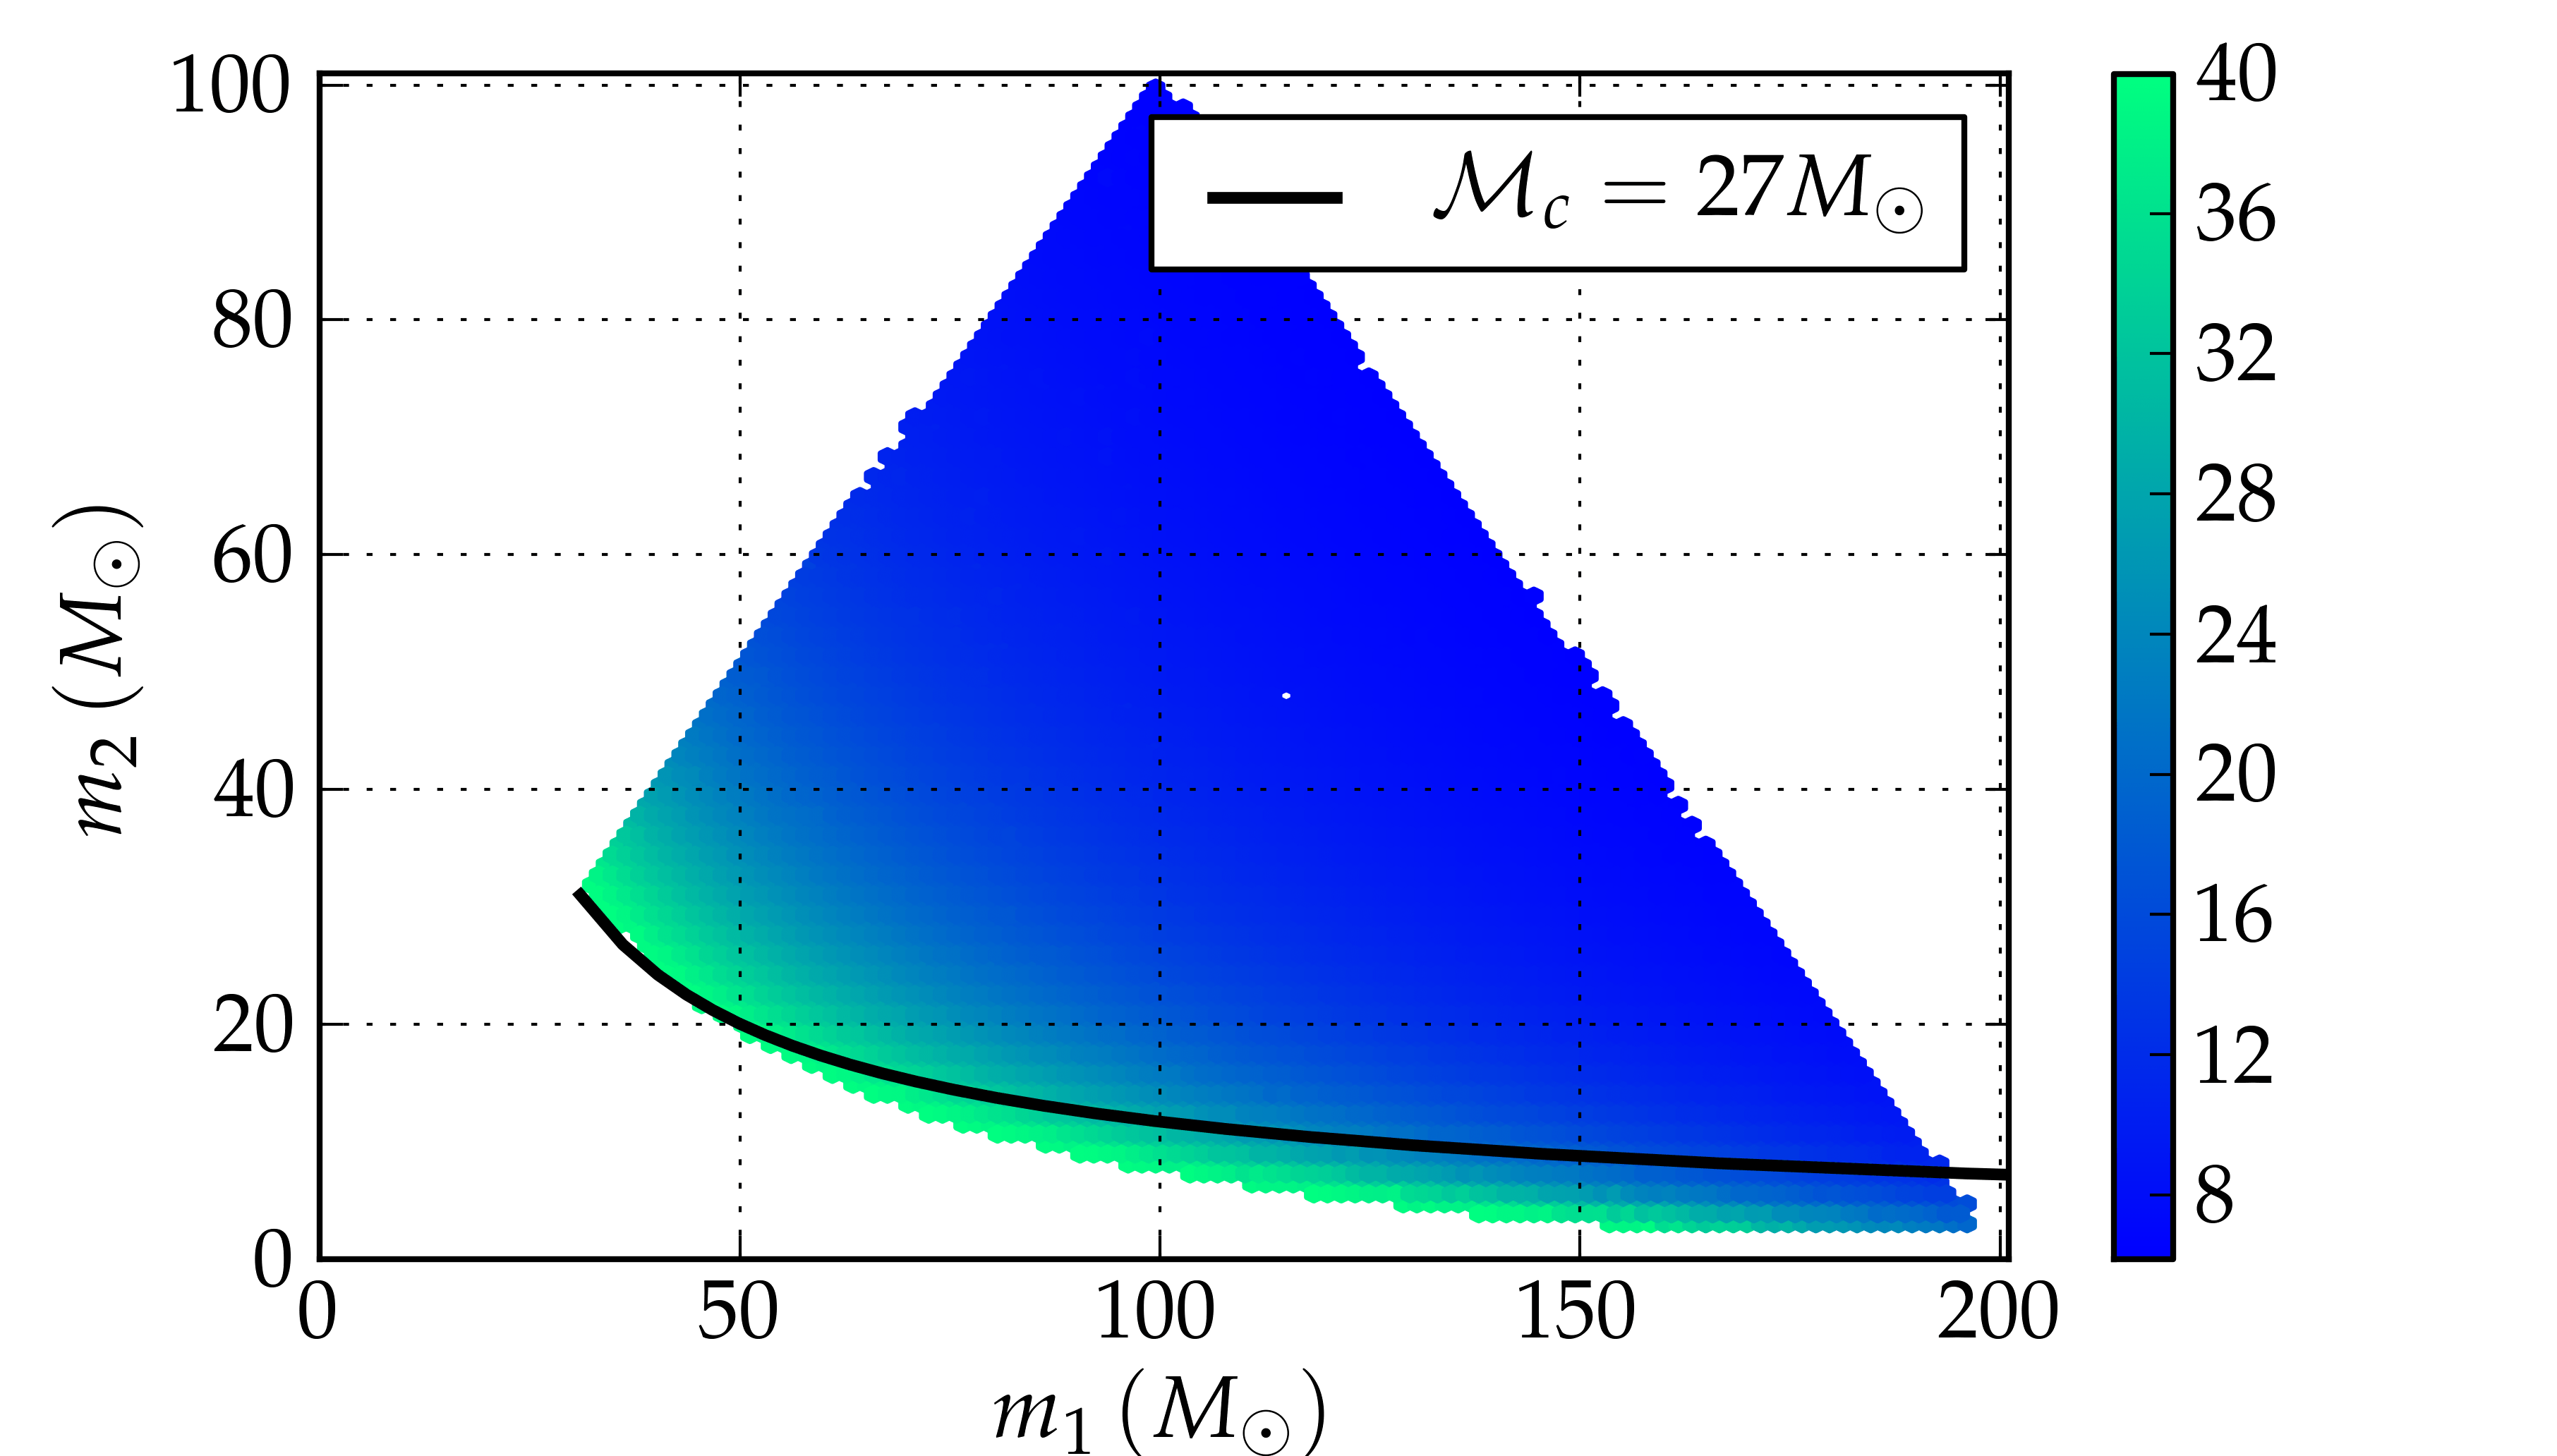
\includegraphics[width=1.1\columnwidth]{BBHm1m2_tlen_Ncyc40_0-99_Mchirp27_cropped-tiny.png}%\quad
%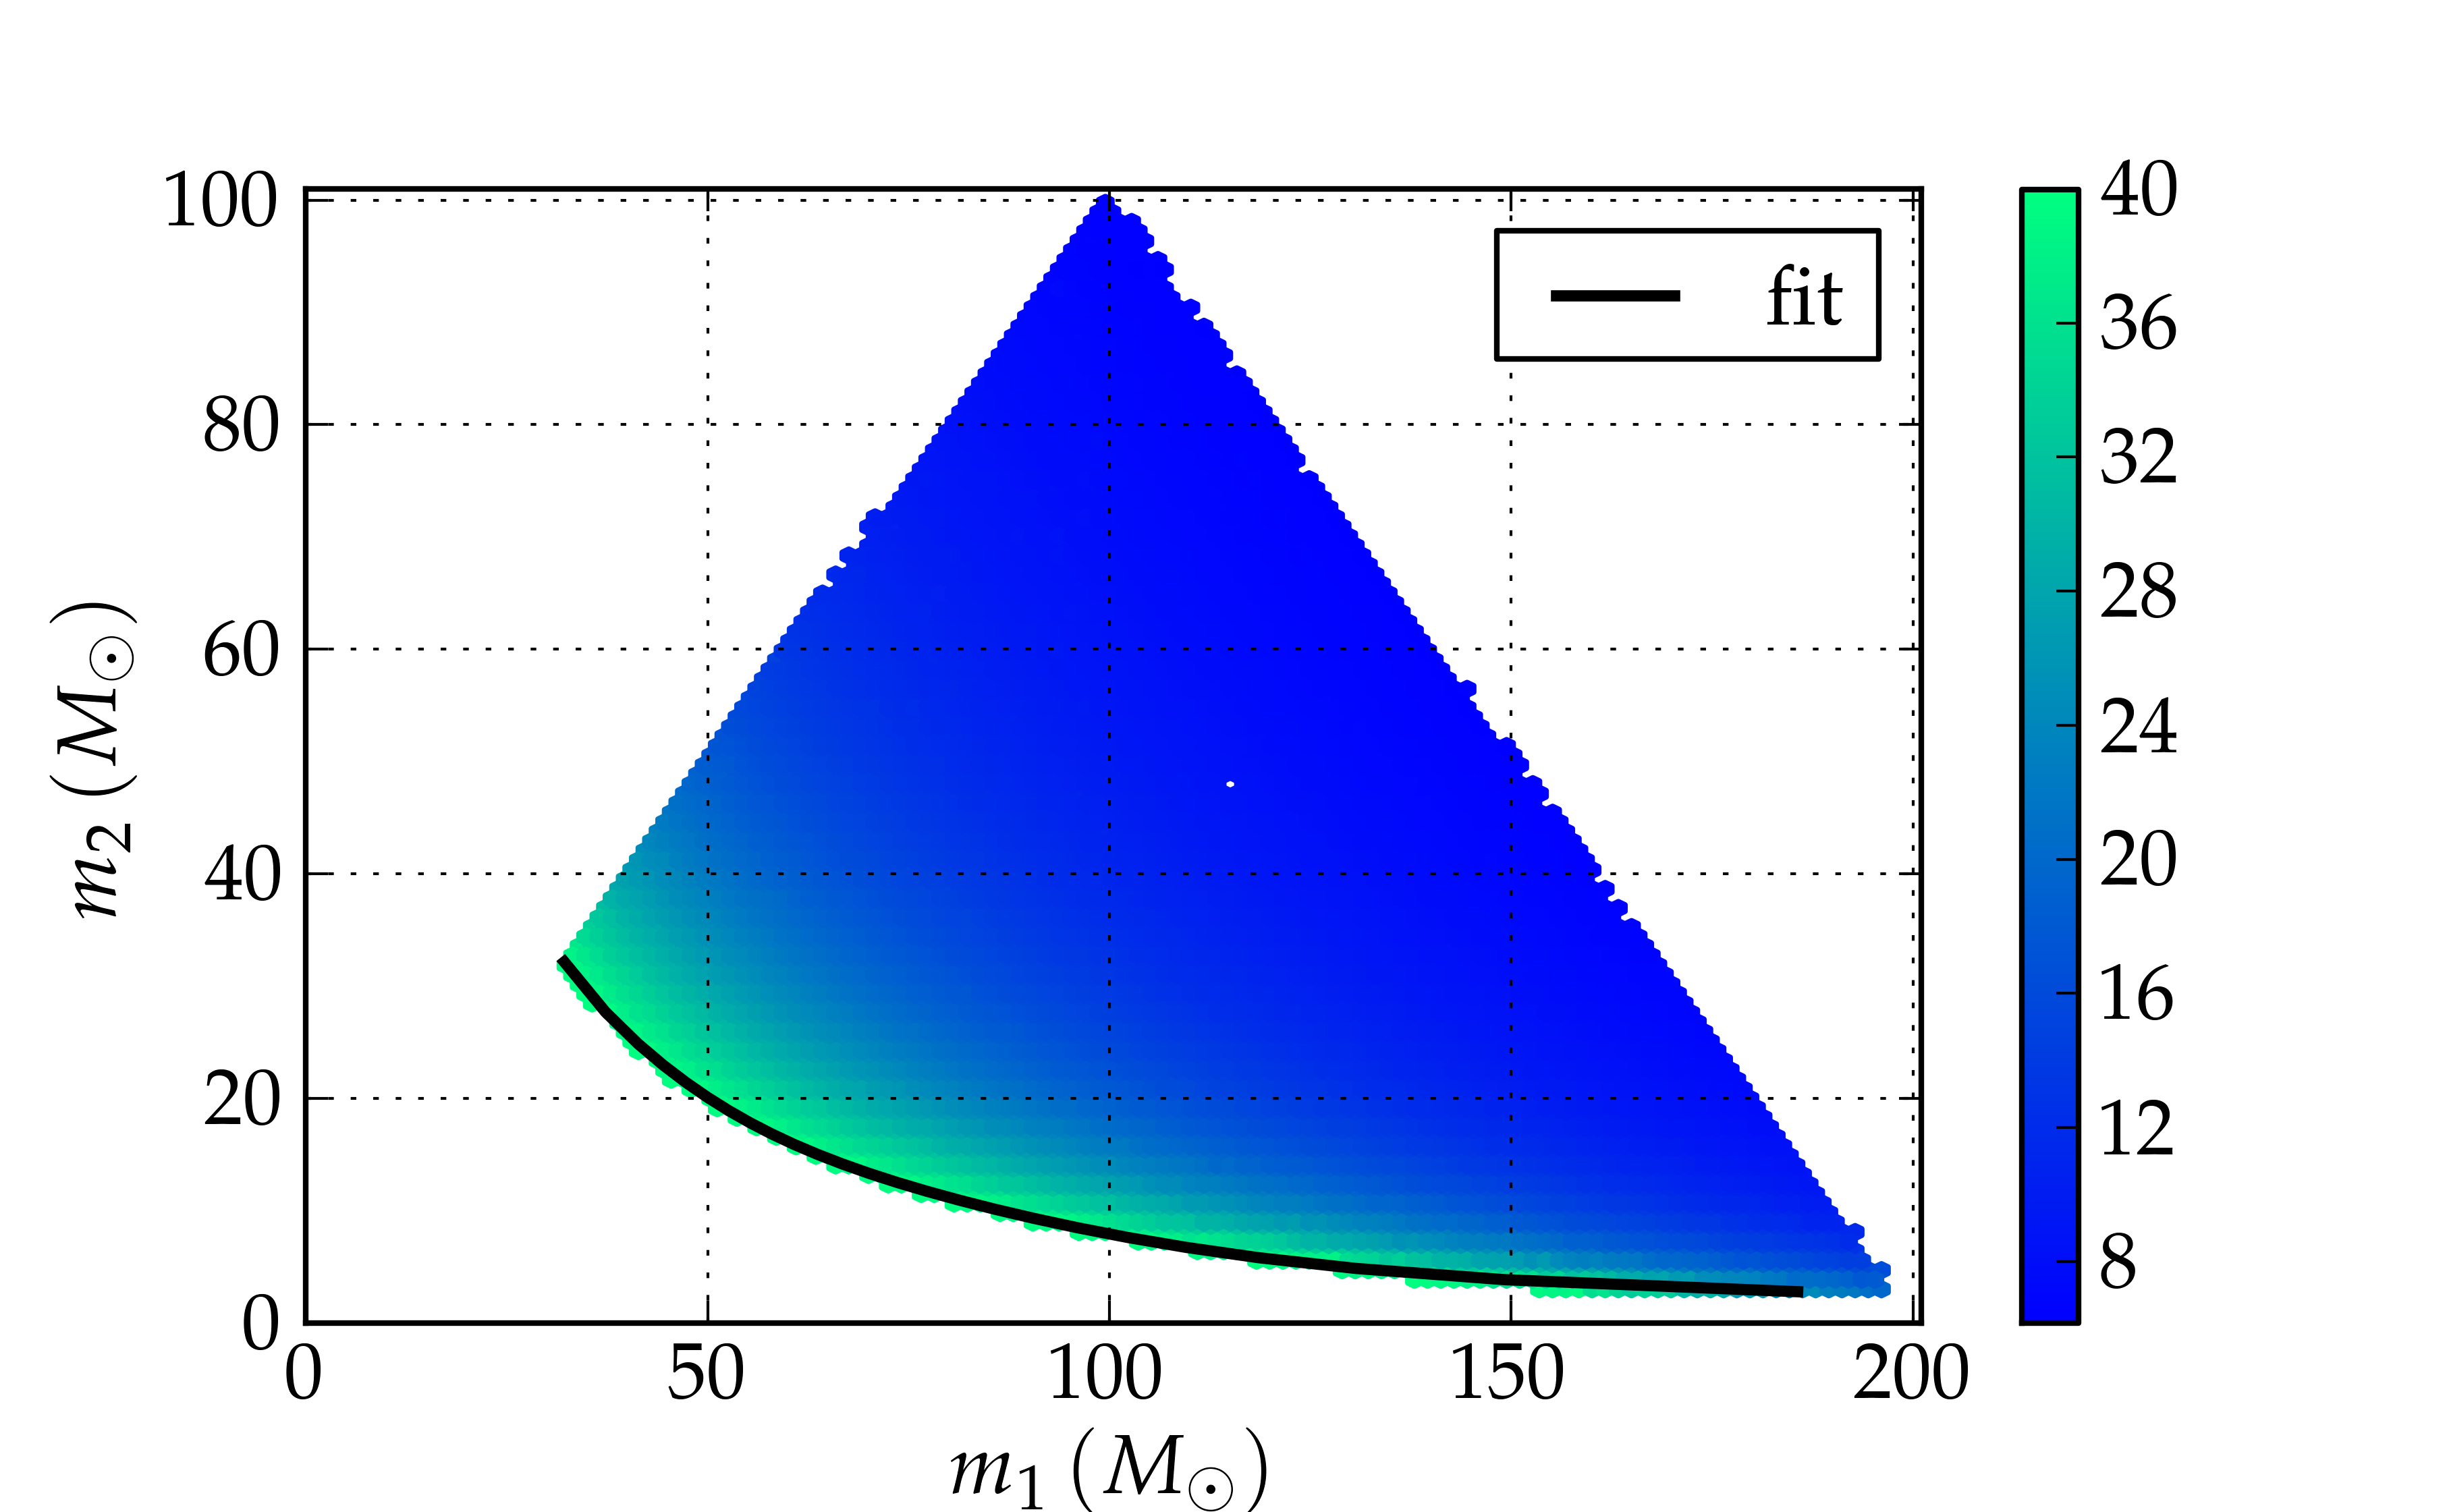
\includegraphics[width=\columnwidth]{BBHm1m2_0-99power_Ncyc40.png}
\caption{The color at each point gives the number 
of waveform cycles $\N_{\cyc}$, for that particular binary, which contain 
$99\%$ of the signal power in the aLIGO sensitivity band. The figure is 
trucated to exclude the region where $\N_{\cyc}>40$. The solid curve shows
the lower bounding edge of the region with $\mathcal{M}_c = 27M_\odot$.}
\label{fig:BBHregion}
\end{figure}

In this section we demonstrate the effectualness of a template bank viable
for using NR waveforms as templates. The gravitational-wave phase of the dominant 
waveform multipole 
extracted from runs at different resolutions was found to converge within 
$\sim 0.3\,\mathrm{rad}$ for $q=3,4,6$, and within $\sim 0.06\,\mathrm{rad}$
for $q=1,2$ at merger (see Fig.~(6) of Ref.~\cite{Buchman:2012dw}, and 
Fig.~(6,7) of Ref.~\cite{BuonannoEOBv2Main} for a compilation). Most of this 
phase disagreement accumulates over a relatively short duration of 
$\sim 50M  - 100M$ before merger, and is significantly lower over the preceding
inspiral and plunge. As the matched-filter SNR accumulates secularly over the
entire waveform, 
these numerical phase errors are negligible in terms of mismatches. We set
$\Gamma_\Hyb = 0$ while computing the fitting factors, so one is left with
considering $\Gamma_\bnk$ to determine the fidelity of the bank (c.f.
Eq.~(\ref{eq:FFGammas})).
% \red{[Harald: These figures compare EOB with NR.  
% How does this imply a statement about the accuracy of the NR waveforms?]}.
% \textcolor{blue}{This was left out at this place by error. The original
% context was the justification of using EOBNRv2 waveforms as
% proxies for NR simulations. I have removed it here.}

With NR simulations as templates, the region that the bank can cover is 
restricted to binaries that have approximately the same number of waveform 
cycles within the sensitive frequency band of the detectors as the simulations
themselves. We take their fiducial length to be $\sim 40$ GW
cycles~\cite{40GWcycles}. For BBHs with 
$3M_{\odot}\leq m_1,m_2\leq 200M_{\odot}$ and $m_1+m_2\leq 200M_{\odot}$ 
we map out the region with $99\%$ of the signal power within $40$ cycles as the
target region of the purely-NR bank. For samples taken over the mass space, we
determine the frequency interval $[f_1,f_2]$ for which
\begin{equation}\label{eq:99percentpower}
 \int_{f_1}^{f_2}\D f \dfrac{|\tilde{h}(f)|^2}{S_n(|f|)} = 
0.99\times\int_{f_\mathrm{min}}^{f_\mathrm{Ny}}\D f \dfrac{|\tilde{h}(f)|^2}{S_n(|f|)}.
\end{equation}
This is done by finding the peak of the integrand in 
Eq.~(\ref{eq:99percentpower}) and integrating symmetrically outwards from 
there, in time, till the interval $[f_1,f_2]$ is found. The number 
of waveform cycles in this interval is
\begin{equation}
 \N_{\cyc} = \dfrac{\Phi( t(f_2) ) - \Phi( t(f_1) )}{2\pi},
\end{equation}
where $\Phi(t)$ is the instantaneous phase of the waveform, 
${h_+(t)\,-\,\ii h_{\times}(t)\,=\,A(t)\,e^{-\ii \Phi(t)}}$, un-wrapped to be a
monotonic function of time. 
We find that for a significant portion of the mass-region, the signal power 
is contained within $40$ waveform cycles. This is shown in 
Fig.~\ref{fig:BBHregion}, where the color at each point gives $\N_{\cyc}$ for
that system, and the region with $\N_{\cyc}> 40$ is excluded. Conservatively, 
this region is bounded by $\mathcal{M}_c = 27M_\odot$, as shown by the solid 
curve in the figure.
% A fit for the total mass $M$ at the lower boundary of this region is given by
% \begin{equation}\label{eq:MtotalFit40Cycles}
% \begin{split}
%  M = \eta^{-3/5}&(12.02 + 217.76\eta - 1469.6\eta^2 + 5169.4\eta^3\\  
%  &-7011.5\eta^4),
%  \end{split}
% \end{equation}
% where $\eta = m_1m_2/M^2 = q/(1+q)^2$ is the symmetric mass-ratio.
% \red{[Harald: Eq (37) is very complicated.  It would be good to
%   give a simpler ``rule-of-thumb''.  By playing around, I found that
%   for the mass-ratios we are interested in, ${\cal M}_c=\mbox{const}$
%   works reasonably well.  I suggest to find the constant, point out that ${\cal M}_c\gtrsim XX$ is an approximation for $q<YY$, and also plot it in Fig. 3.]}


We place a bank over this region, using a stochastic method similar 
to Ref.~\citep{Harry:2009ea,Ajith:2012mn,Manca:2009xw}. 
The algorithm begins by taking an empty bank,
corresponding to step $0$. At step $i$, a proposal point $(q,M)$ is picked
by first choosing a value for $q$ from the restricted set
$\mathcal{S}_q=\{1,2,3,4,6,8\}$. The total mass $M$ is subsequently sampled
from the restricted interval corresponding to the pre-drawn $q$. The proposal 
is accepted if the waveform at this point has overlaps $\mathcal{O}< 0.97$ 
with all the templates in the bank from step $i-1$. This gives 
the bank at step $i$. The process is repeated till the fraction of 
proposals being accepted falls below $\sim 10^{-4}$, and $\gtrsim 99\%$
of the parameter space is covered effectually.
% \red{[Harald: I would have expected that by the time such a small acceptance fraction is reached, the bank is complete.  Is there a simple explanation why not?]}
% \textcolor{blue}{The acceptance rate decreases extremely rapidly as the bank
% converges to $> 99\%$ coverage fraction. This was shown in
% http://arxiv.org/abs/0908.2090 (Table II and Fig. 9). Table II
% shows that an acceptance ratio of $1$ in $10^4$ is achieved close to a 
% coverage fraction of $99.9\%$, while sampling in $\tau_0 - \tau_3$ coordinates.
% We can expect it to be lower for us as we sampled in $\mathcal{M}_c - \eta$ 
% coordinates.}
To complete the coverage, $100,000$ points are sampled over the region of mass
space depicted in Fig.~\ref{fig:BBHregion}, and $\FF$ of the bank
is computed at each point. With the islands of undercoverage isolated, the
points sampled in these regions are added to the bank, pushing their 
mass-ratios to the two neighboring mass-ratios in $\mathcal{S}_q$ 
along lines of constant chirp mass. 
This helps accelerate the convergence of the bank, albeit at the cost of 
over-populating it, as the algorithm for computing the $\FF$ for the 
sampled points is parallelizable.
\begin{figure}
\centering
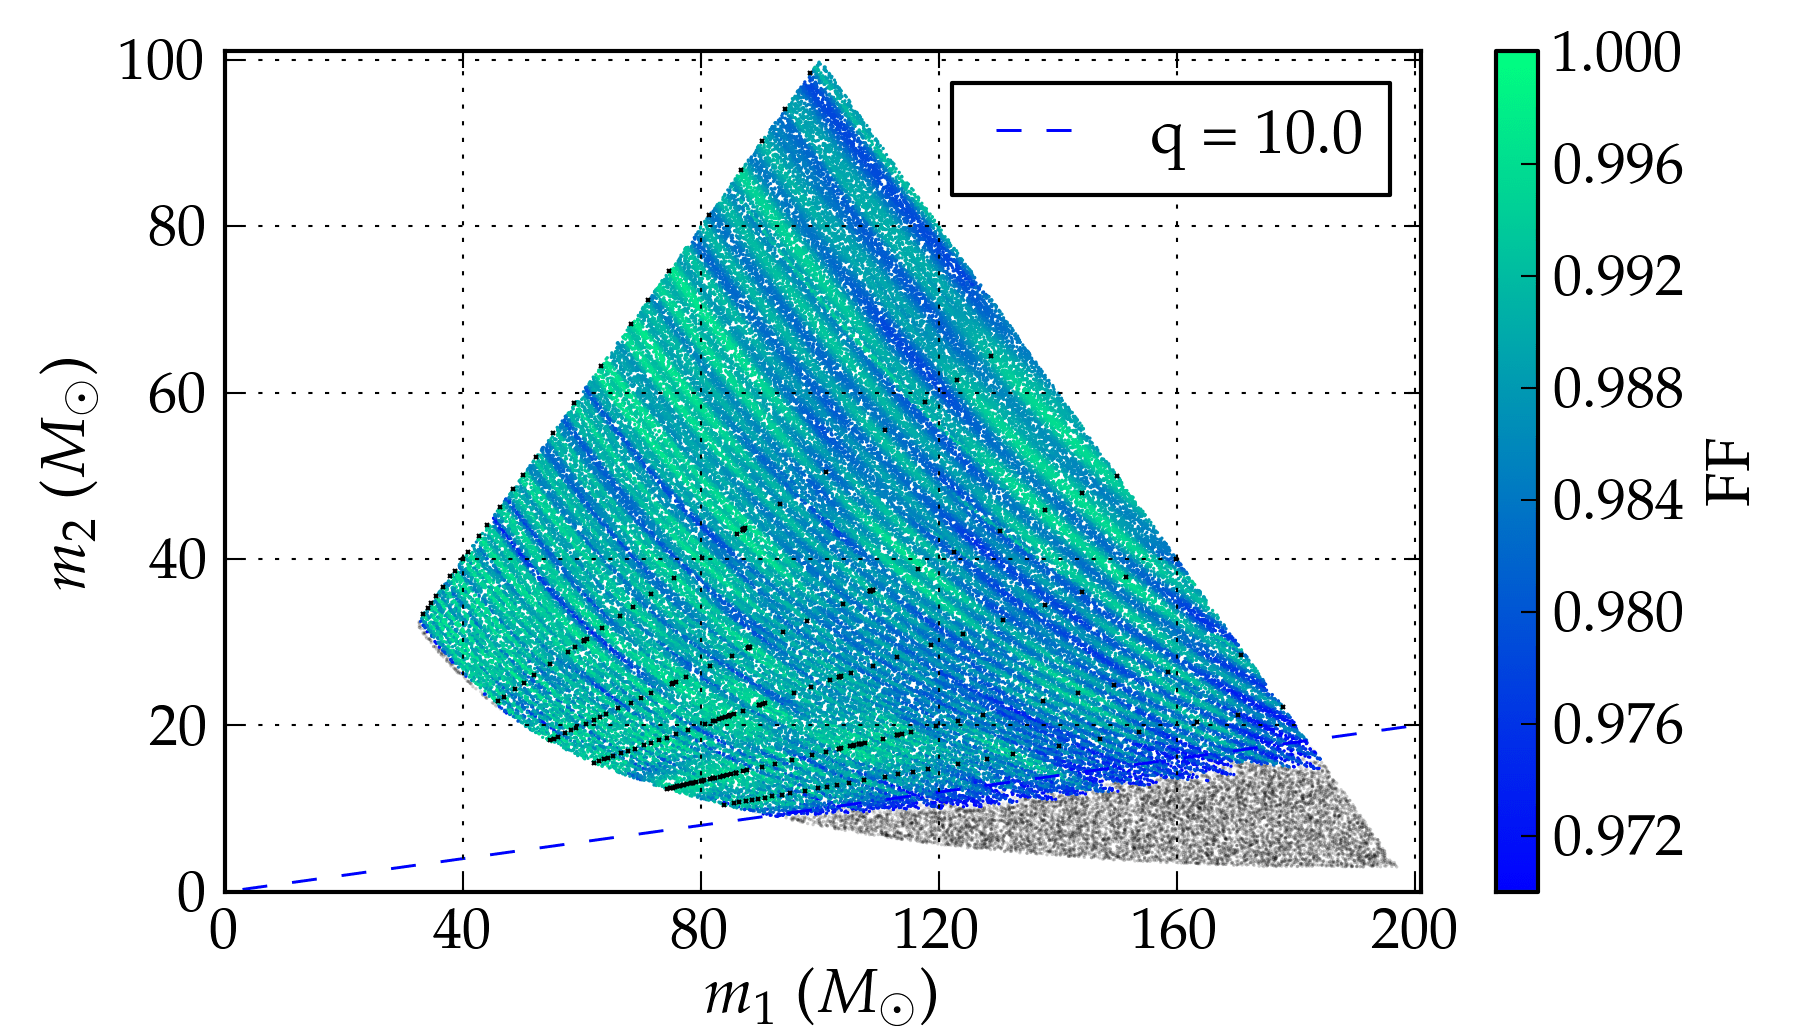
\includegraphics[width=\columnwidth]{bank002_01_01_mtot200_match_cropped-tiny.png}
%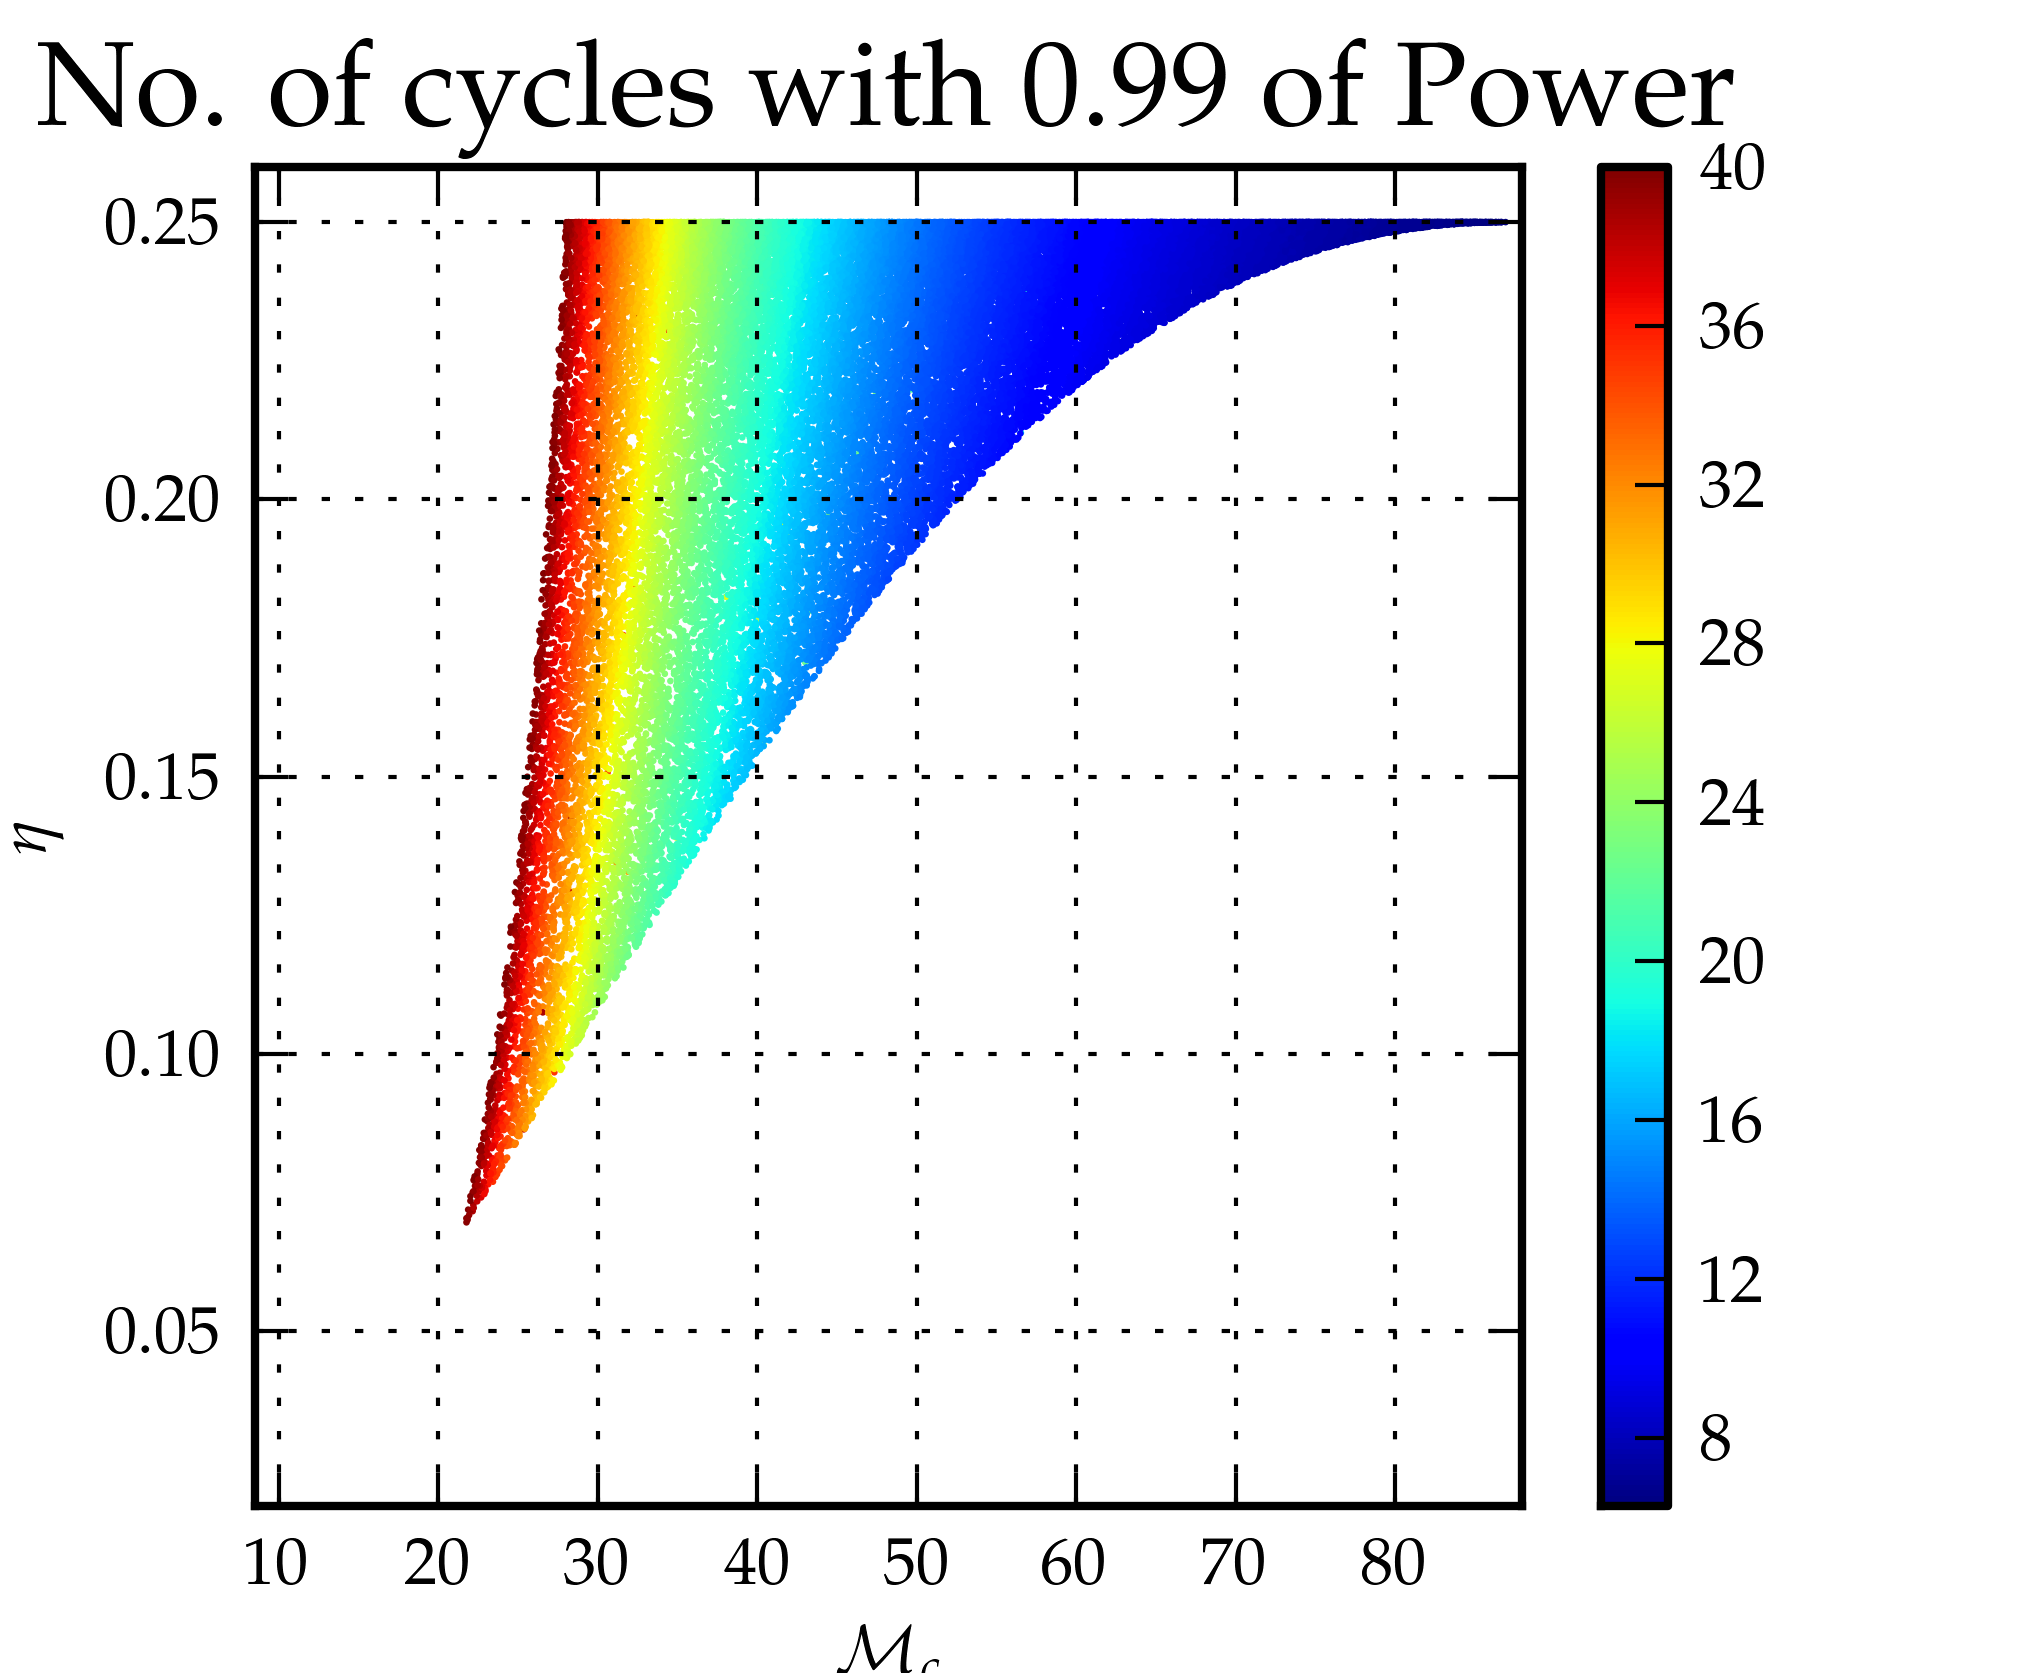
\includegraphics[width=\columnwidth]{BBHmcet_0-99power_Ncyc40.png}
\caption{The color at each point in the figure gives the
value of $\FF\simeq 1-\Gamma_{\bnk}$ of the bank for that binary, for
the NR bank restricted to $\mathcal{S}_q=\{1,2,3,4,6,8\}$. This is the
same as the fraction of the optimal SNR, for the binary, that the
template bank recovers. The black dots show
the location of the templates in the bank. We note that they all lie
along straight lines of constant $q$ passing through the origin. The region 
shaded light-grey (towards the bottom of the figure) is where the $\FF$ 
drops sharply below $97\%$.}
\label{fig:bank001_01_match}
\end{figure}
\begin{figure}
\centering
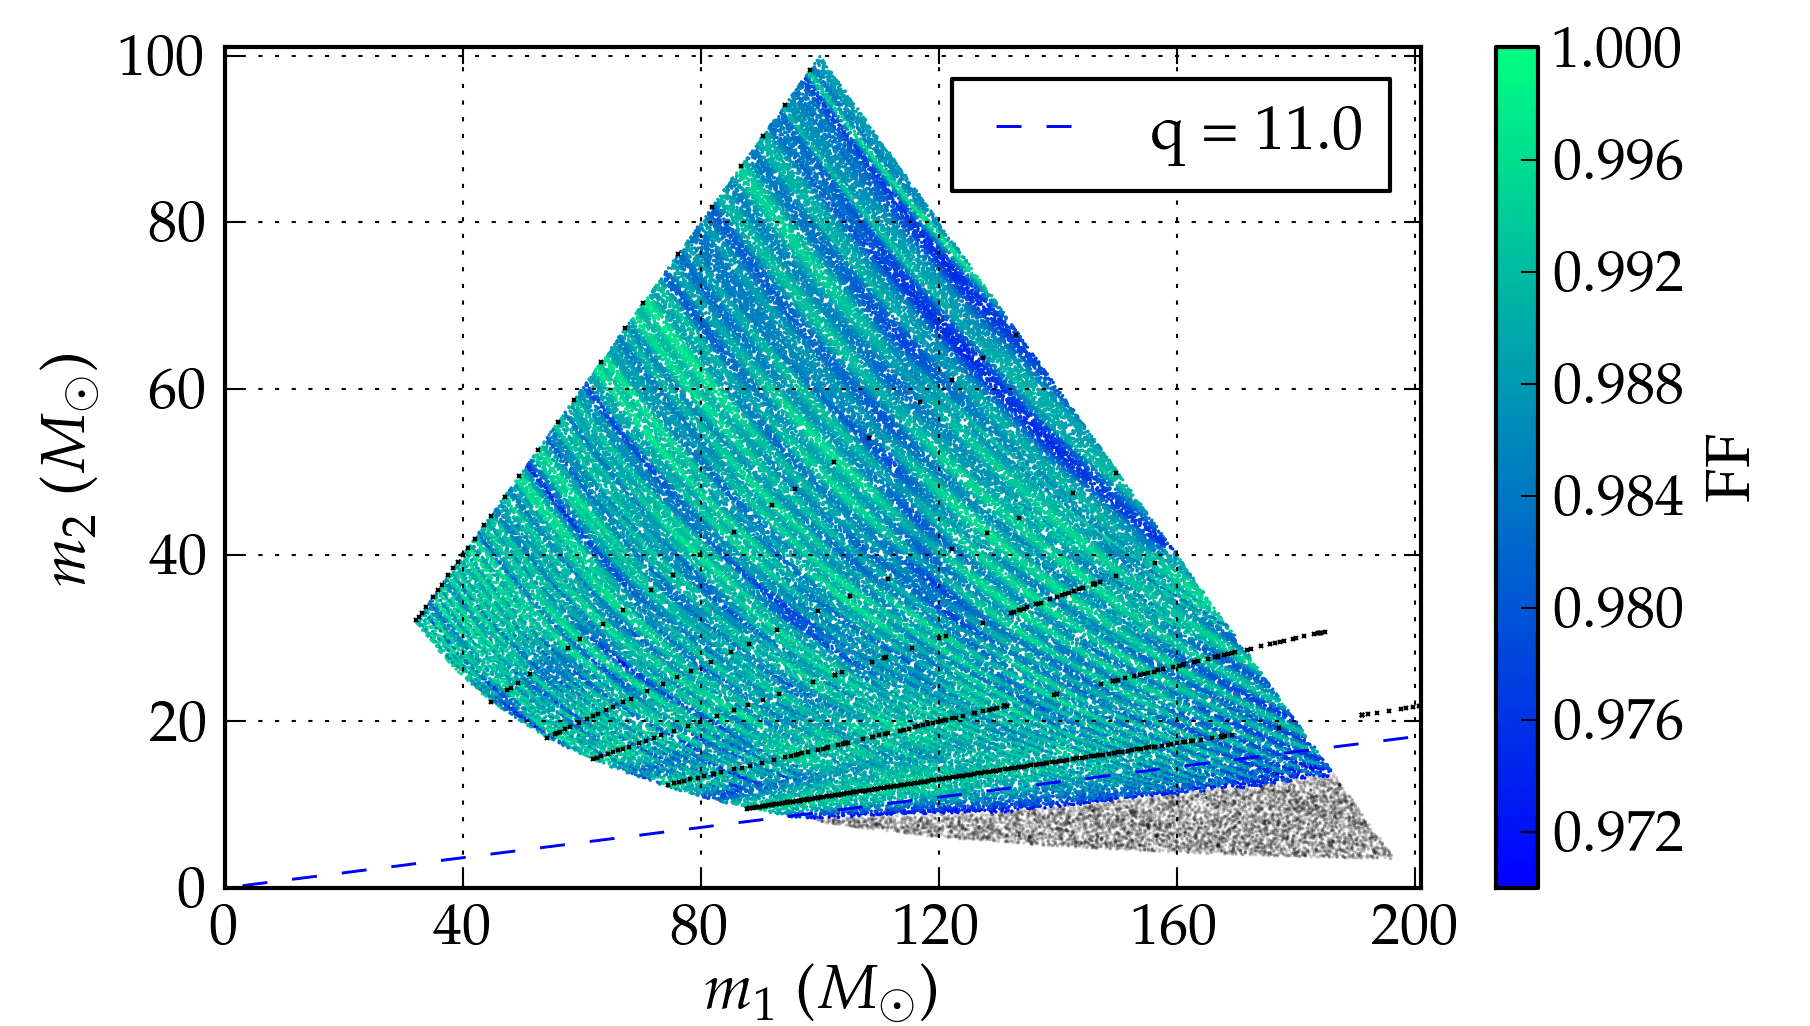
\includegraphics[width=\columnwidth]{bank006_01_mtot200_match_cropped-tiny.png}
%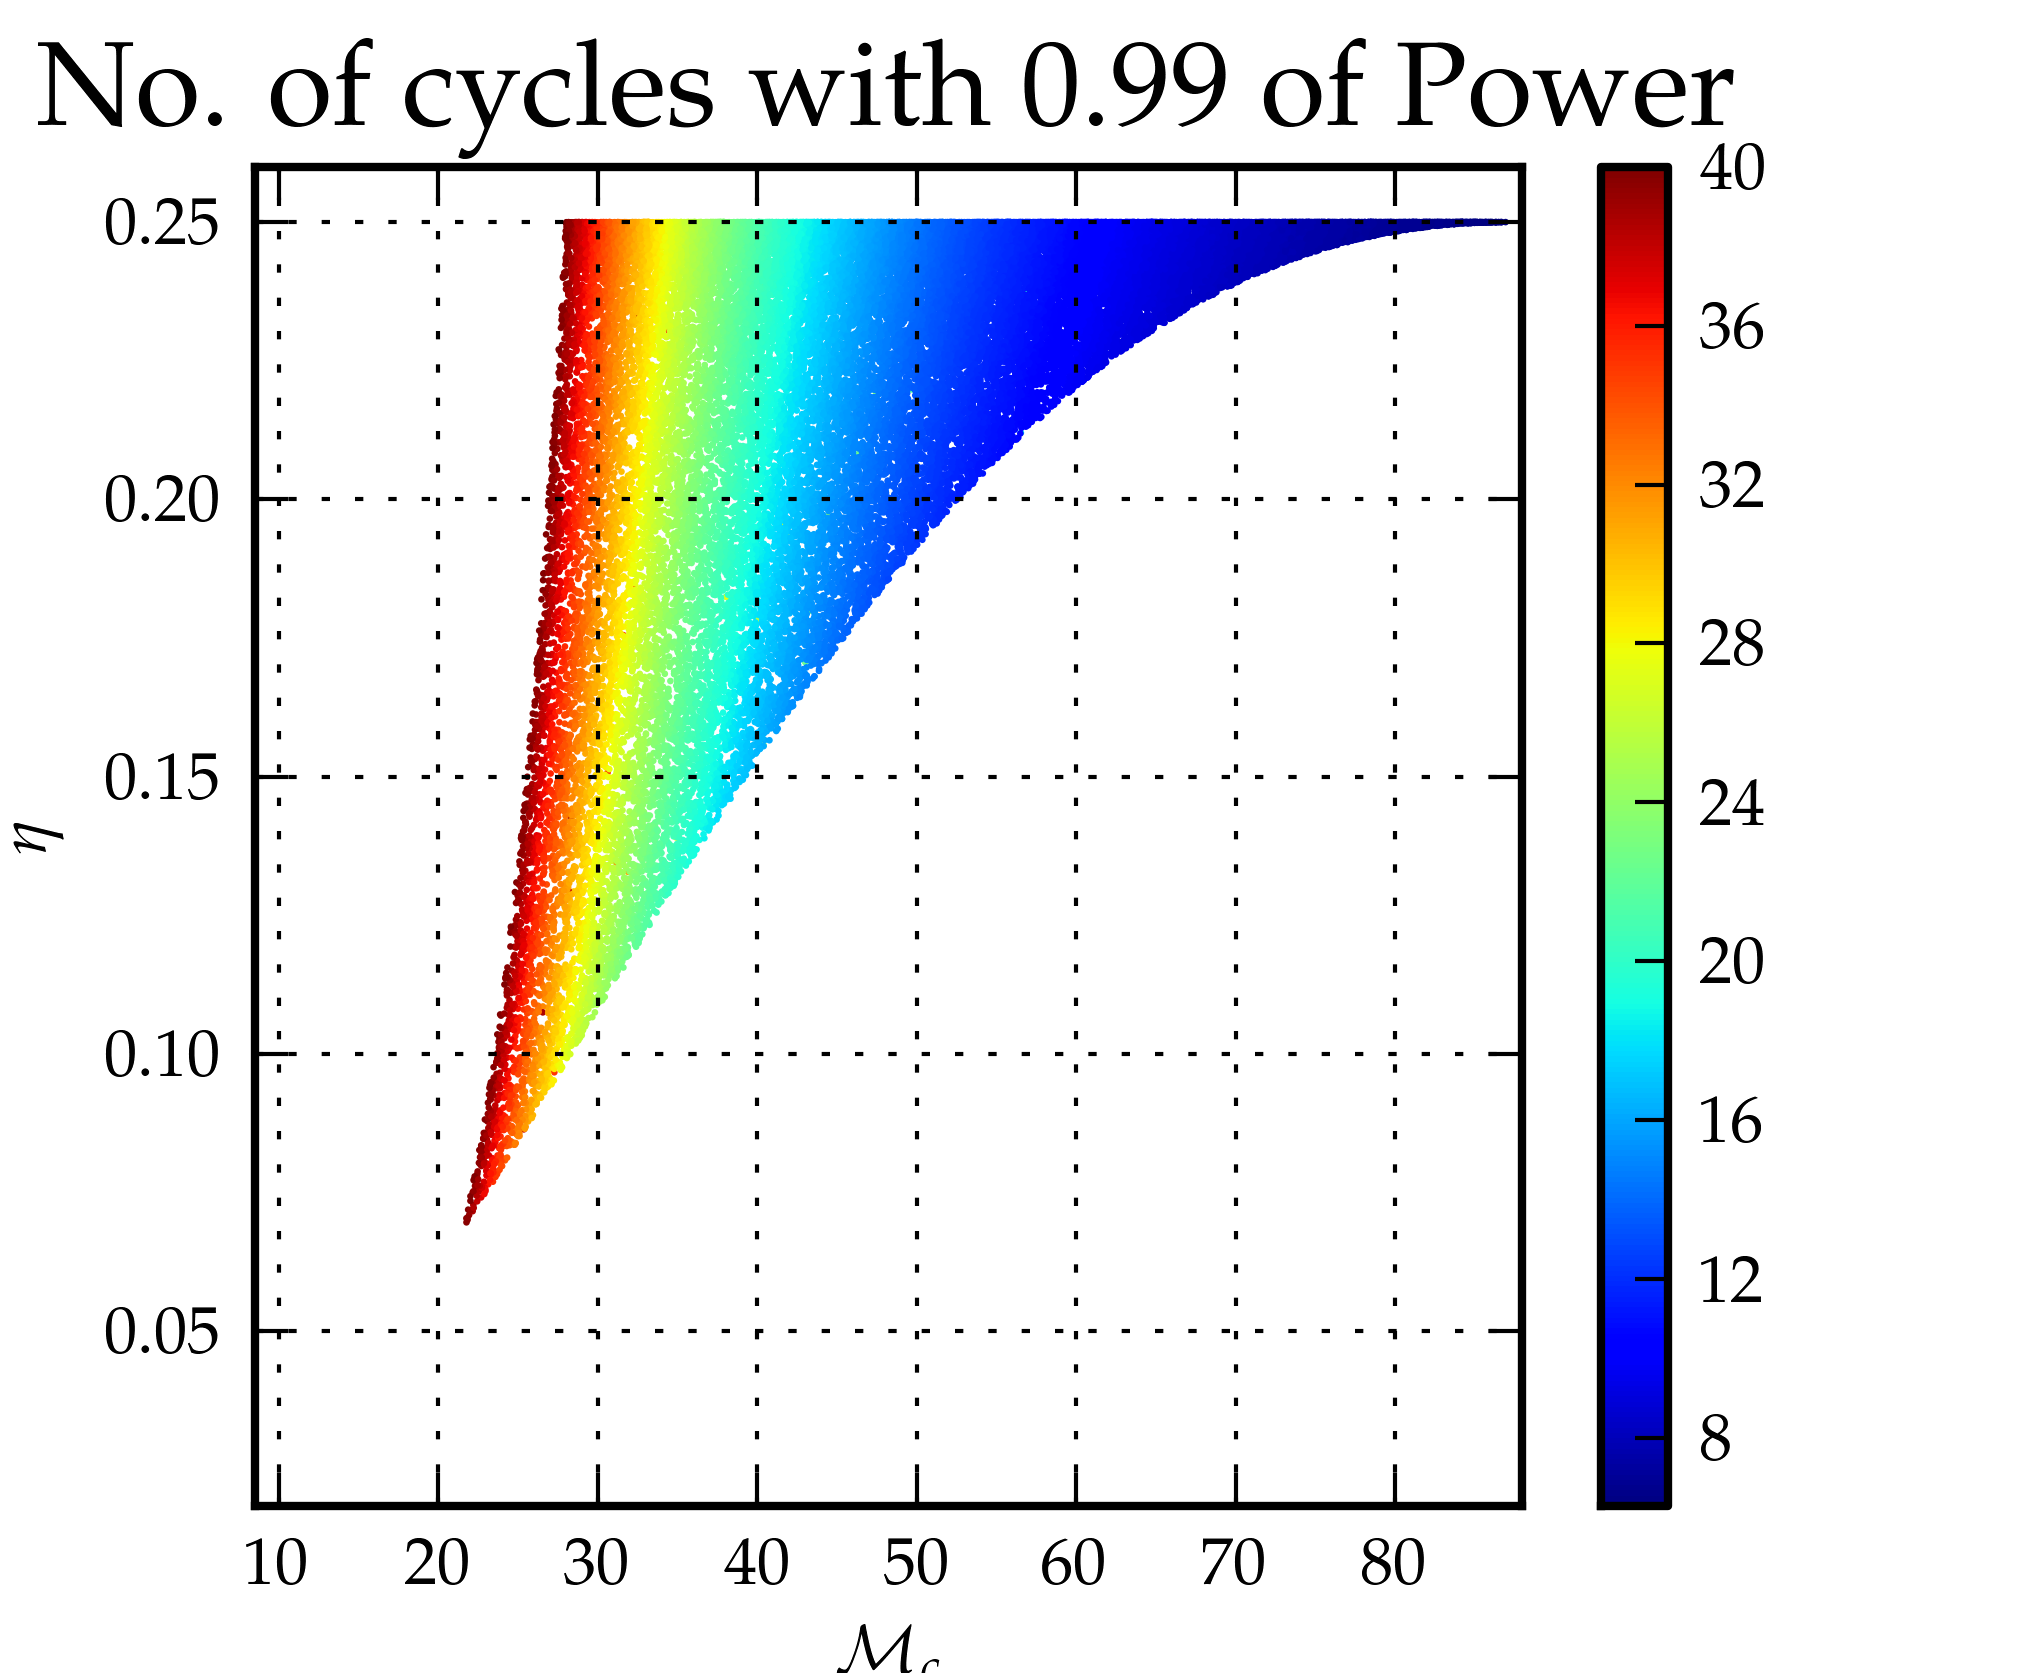
\includegraphics[width=\columnwidth]{BBHmcet_0-99power_Ncyc40.png}
\caption{This figure is similar to Fig.~\ref{fig:bank001_01_match}.
The color at each point gives the value of 
$\FF\simeq 1-\Gamma_{\bnk}$ of the bank for that binary, for
the NR bank restricted to $\mathcal{S}_q=\{1,2,3,4,6,9.2\}$.
The black dots show the location of the templates in the bank. 
The region shaded light-grey (towards the bottom of the figure) is 
where the $\FF$ drops below $97\%$. We note that with an additional
NR waveform for mass ratio $q=9.2$, the coverage of the bank is 
extended to include binaries with $10\leq q\leq 11$.}
\label{fig:bank006_01_match}
\end{figure}
% We test the bank so constructed by measuring the loss in the SNR that the 
% bank incurs for arbitrary incoming GW signals. As the waveform 
% mismatches due to the numerical errors are negligibly small, the primary cause
% for the loss in SNR would be the discreteness of the template bank grid. This
% effect can be measured by simulating BBH waveforms for various systems sampled
% over the region of the mass-parameter space that the bank intends to cover, and
% computing the fraction of optimal SNR that is recovered when these signals are
% filtered with our bank. 
% We need the signals and templates to be in the same
% manifold, to measure the effect of the discreteness of the bank alone.
% The recently proposed EOBNRv2 approximant~\cite{BuonannoEOBv2Main} was 
% calibrated to the numerical simulations for $q=\{1,2,3,4,6\}$, and thus 
% provides an excellent ground for that, i.e. superscript M~=~EOBNRv2 in
% $\Gamma_{\bnk}$ (Eq.~\ref{eq:FFConstraint}).

We asses the effectualness of the bank, as discussed in 
Sec.~\ref{s1:quantifyingerrors}, using Eq.~(\ref{eq:NRFFGammas}).
We draw a population of $100,000$ BBH signals, uniformly from the binary 
mass space, and filter them through the bank. Fig.~\ref{fig:bank001_01_match}
shows the $\FF$, or the fraction of the optimal SNR recovered by the bank. 
The region shown is restricted to binaries with $N_{\cyc}\leq 40$.
The black dots in the figure show the position of templates in the bank. 
The bank recovers $\geq 97\%$ of the optimal SNR over the entire region 
of interest for $q\leq 10$. We 
propose an additional simulation for $q=9.2$, to increase the coverage to
higher mass-ratios. Substituting this for $q=8$ in the set of allowed 
mass-ratios $\mathcal{S}_q$, we place another bank as before, with
$\mathcal{S}_q=\{1,2,3,4,6,9.2\}$. The SNR loss from this bank is shown in
Fig.~\ref{fig:bank006_01_match}. This bank recovers $\geq 97\%$ of the SNR for
systems with $q\leq 11$ and $\N_{\cyc}\leq 40$. The choice of the additional
simulation at $q=9.2$ was made by choosing a value \textit{close-to} the 
highest possible value of $q$ that does not lead to under-coverage in the 
region between $q=6$ and that value. The \textit{exact} highest allowed 
value was not chosen to reduce the sensitivity of the coverage of the bank
to fluctuations in detector sensitivity.

We conclude that with only six NR waveforms for non-spinning BBHs, that are
$\sim 20$ orbits (or $40$ GW cycles) in length, a template bank can be
constructed that is effectual for detecting binaries with chirp mass above
$27M_\odot$ and $1\leq q\leq 10$. With an additional 
simulation for $q=9.2$, this bank can 
be extended to higher mass-ratios, i.e. to $1\leq q\leq 11$.



\subsection{NR-pN hybrid template bank}\label{s2:NRpNhybridbank}

%\textcolor{red}{Why do we need a bank of hybrids?}\newline
The template bank contructed in Sec.~\ref{s1:NRonlybank} is effectual for 
GW detection searches focussed at relatively massive binaries with 
$\mathcal{M}_c \gtrsim 27M_\odot$. As the NR waveforms are restricted to a
small number of orbits, it is useful to consider NR-PN hybrids to bring the
lower mass limit down on the template bank. PN waveforms can be generated
for an arbitrarily large number of inspiral orbits, reasonably accurately and
relatively cheaply. Thus, a hybrid waveform comprised of a long PN early-inspiral 
and an NR late-inspiral, merger, and ringdown could also be arbitrarily long. 
There are, however, uncertainties in the PN waveforms, due to
the unknown higher-order terms. During the late-inspiral and merger phase,
these terms become more important and the PN description becomes
less accurate. In addition, when more of the late-inspiral is
in the detector's sensitivity frequency range, hybrid waveform mismatches 
due to the PN errors become increasingly large, and reduce the
recovered SNR. Thus, when
hybridizing PN and NR waveforms, there must be enough NR orbits that the PN
error is sufficiently low for the considered detector noise-curve. In 
this section, we construct an NR + PN hybrid template bank, for currently
available NR waveforms, and determine the lowest value of binary masses to 
which it covers.


%\subsubsection{Including hybrid PN error}\label{s2:HybridPNerror}
\begin{figure}
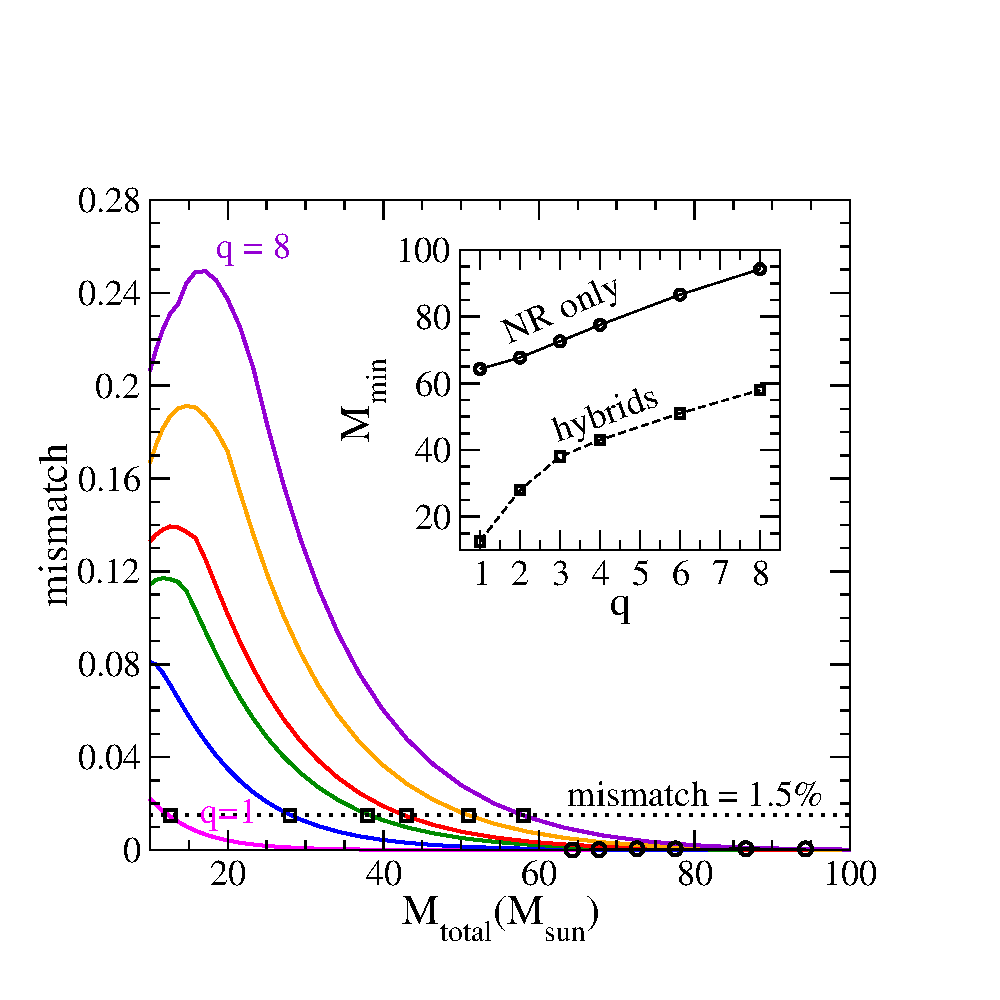
\includegraphics[width=0.9\columnwidth, trim=20 17 75 75]{maxmismatchVSmass_allq.pdf}
\caption{\label{fig:Current-NR-PN-Errors}Bounds on mismatches of PN-NR
  hybrid waveforms, for the currently existing NR simulations. The PN
  error is for hybrids matched at $M\omega_m=0.025$ for $q=1$,
  $M\omega_m=0.038$ for $q=2$, and $M\omega_m=0.042$ for
  $q=3,4,6,8$. The black circles indicate the lower bound of the
  template bank in Sec.~\ref{s1:NRonlybank}. The black square show the
  lower bound with a hybrid error of 1.5\%. The inset shows these
  lower bounds as a function of mass ratio.} 
\end{figure}

%\textcolor{red}{Details of hybrids and how we estimate their errors?}\newline
The hybrids we use are constructed by joining the PN and NR portions, as 
described in Sec.~\ref{s2:NRpNhybridwaveforms}. The number of orbits before 
merger at which they are joined depends on the length of the available NR 
waveforms. We estimate the PN waveform errors using hybridization
mismatches $\Gamma_\Hyb$, as discussed in Sec.~\ref{s1:quantifyingerrors}. 
Fig.~\ref{fig:Current-NR-PN-Errors} shows the same for all the hybrids, as a 
function of total mass. In terms of orbital frequency, these are
matched at $M\omega_m=0.025$ for $q=1$, $M\omega_m=0.038$ for $q=2$,
and $M\omega_m=0.042$ for $q=3,4,6,8$. In terms of number of orbits
before merger, this is 31.9 orbits for $q=1$, 17.8 orbits for $q=2$,
16.9 orbits for $q=3$, 18.4 orbits for $q=4$, 21.6 orbits for $q=6$,
and 25.1 orbits for $q=8$. The dotted line indicates a mismatch of
$1.5\%$, a comparatively tight bound that leaves flexibility to accommodate
errors due to template bank discreteness. The black circles show the hybrid
mismatches at the lower mass bound of the NR-only template bank in
Sec.~\ref{s1:NRonlybank}, which are negligible. The inset shows this minimum 
mass as a function of mass ratio, as well as the minimum attainable mass if we
accept a hybrid error of $1.5\%$. At lower masses, the mismatches increase
sharply with more of the PN part moving into the Advanced LIGO sensitivity band.
This is due to the nature of the frequency dependence of the detector 
sensitivity. The detectors will be relatively very sensitive to a relatively 
short frequency band. As the hybridization frequency sweeps through that band, 
the hybrid errors rise sharply. They fall again at the lowest masses, for which
mostly the PN portion stays within the sensitive band.


\begin{figure*}
\begin{center}
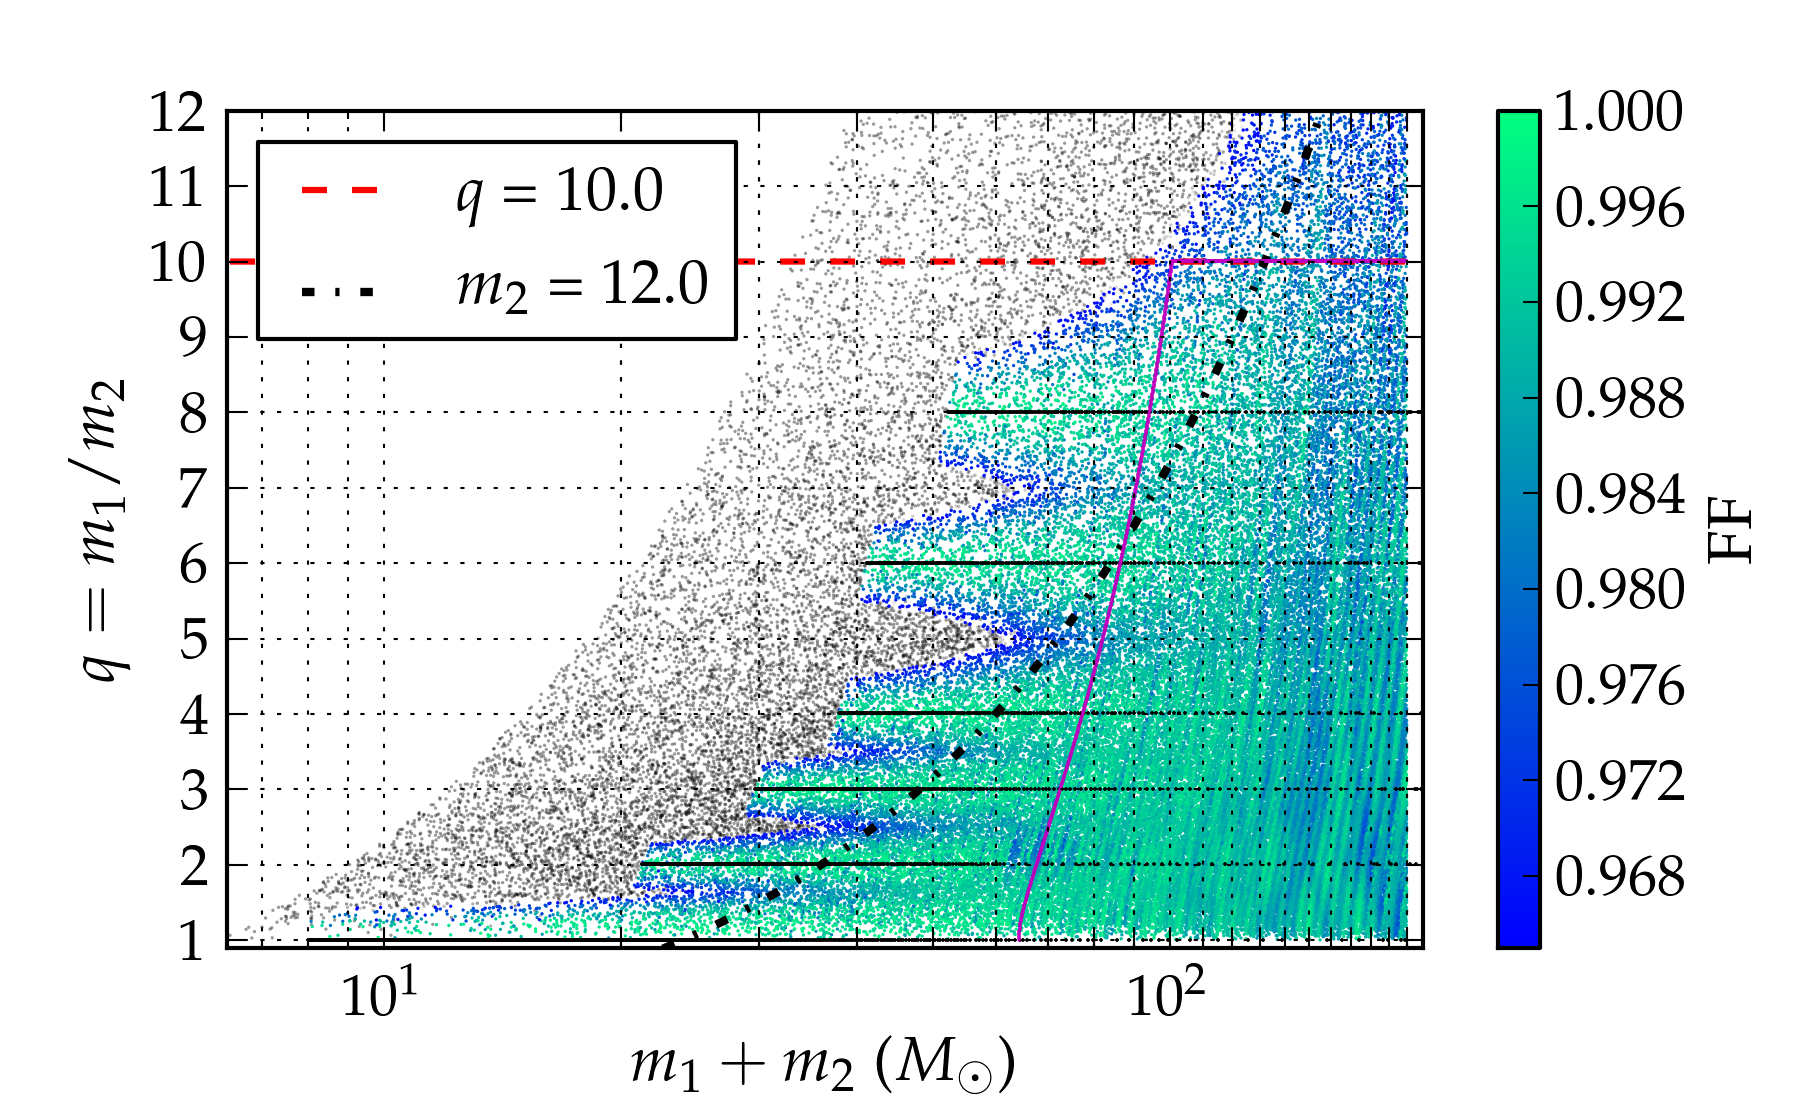
\includegraphics[width=\columnwidth]{bank001_lowM_01_stochastic_mtot200_logMq_NOhybMM.png}
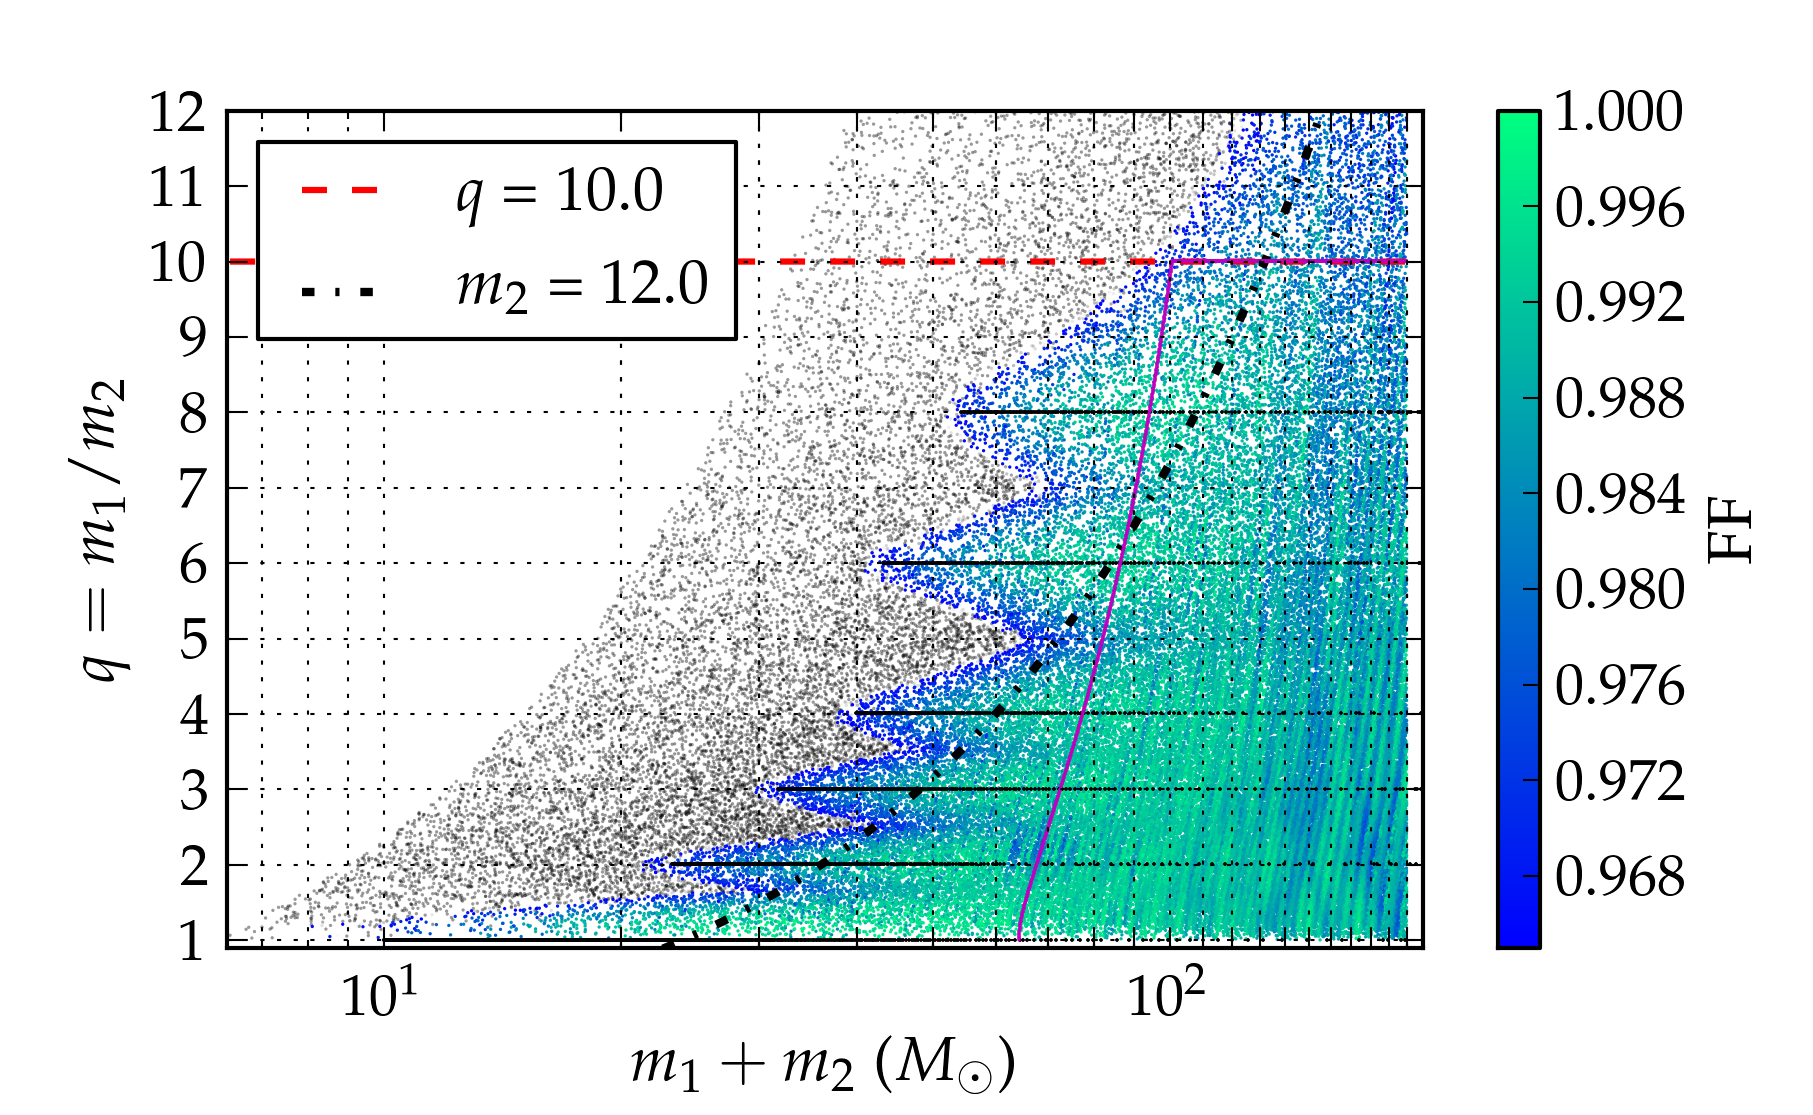
\includegraphics[width=\columnwidth]{bank001_lowM_01_stochastic_mtot200_logMq_hybMM.png}
\caption{\label{fig:Current-hybrids-stochastic-FF}These figures show fitting
  factors $\FF$ obtained when using a discrete mass-ratio template bank for
  $q=1,2,3,4,6,8$. For each mass-ratio, the templates are extended down 
  to a total mass where the NR-PN hybridization mismatch becomes
  $3\%$. The bank is placed using the stochastic algorithm, similar to 
  Ref.~\cite{Harry:2009ea,Ajith:2012mn,Manca:2009xw}. 
  The black dots show the location
  of the templates. The fitting factor on the left plot does 
  {\em not} take into account the hybridization error, and therefore shows the
  effect of the sparse placement of the templates alone. 
  The right plot accounts for the hybridization error
  and gives the actual fraction of the optimal SNR that would be recovered
  with this bank of NR-PN hybrid templates. The region bounded by the magenta 
  (solid) line in both plots indicates the lower end of the coverage of the 
  bank of un-hybridized NR waveforms. Lastly, the shaded grey dots show the 
  points where the fitting factor was below $96.5\%$.}
\end{center}
\end{figure*}
\begin{figure*}
\begin{center}
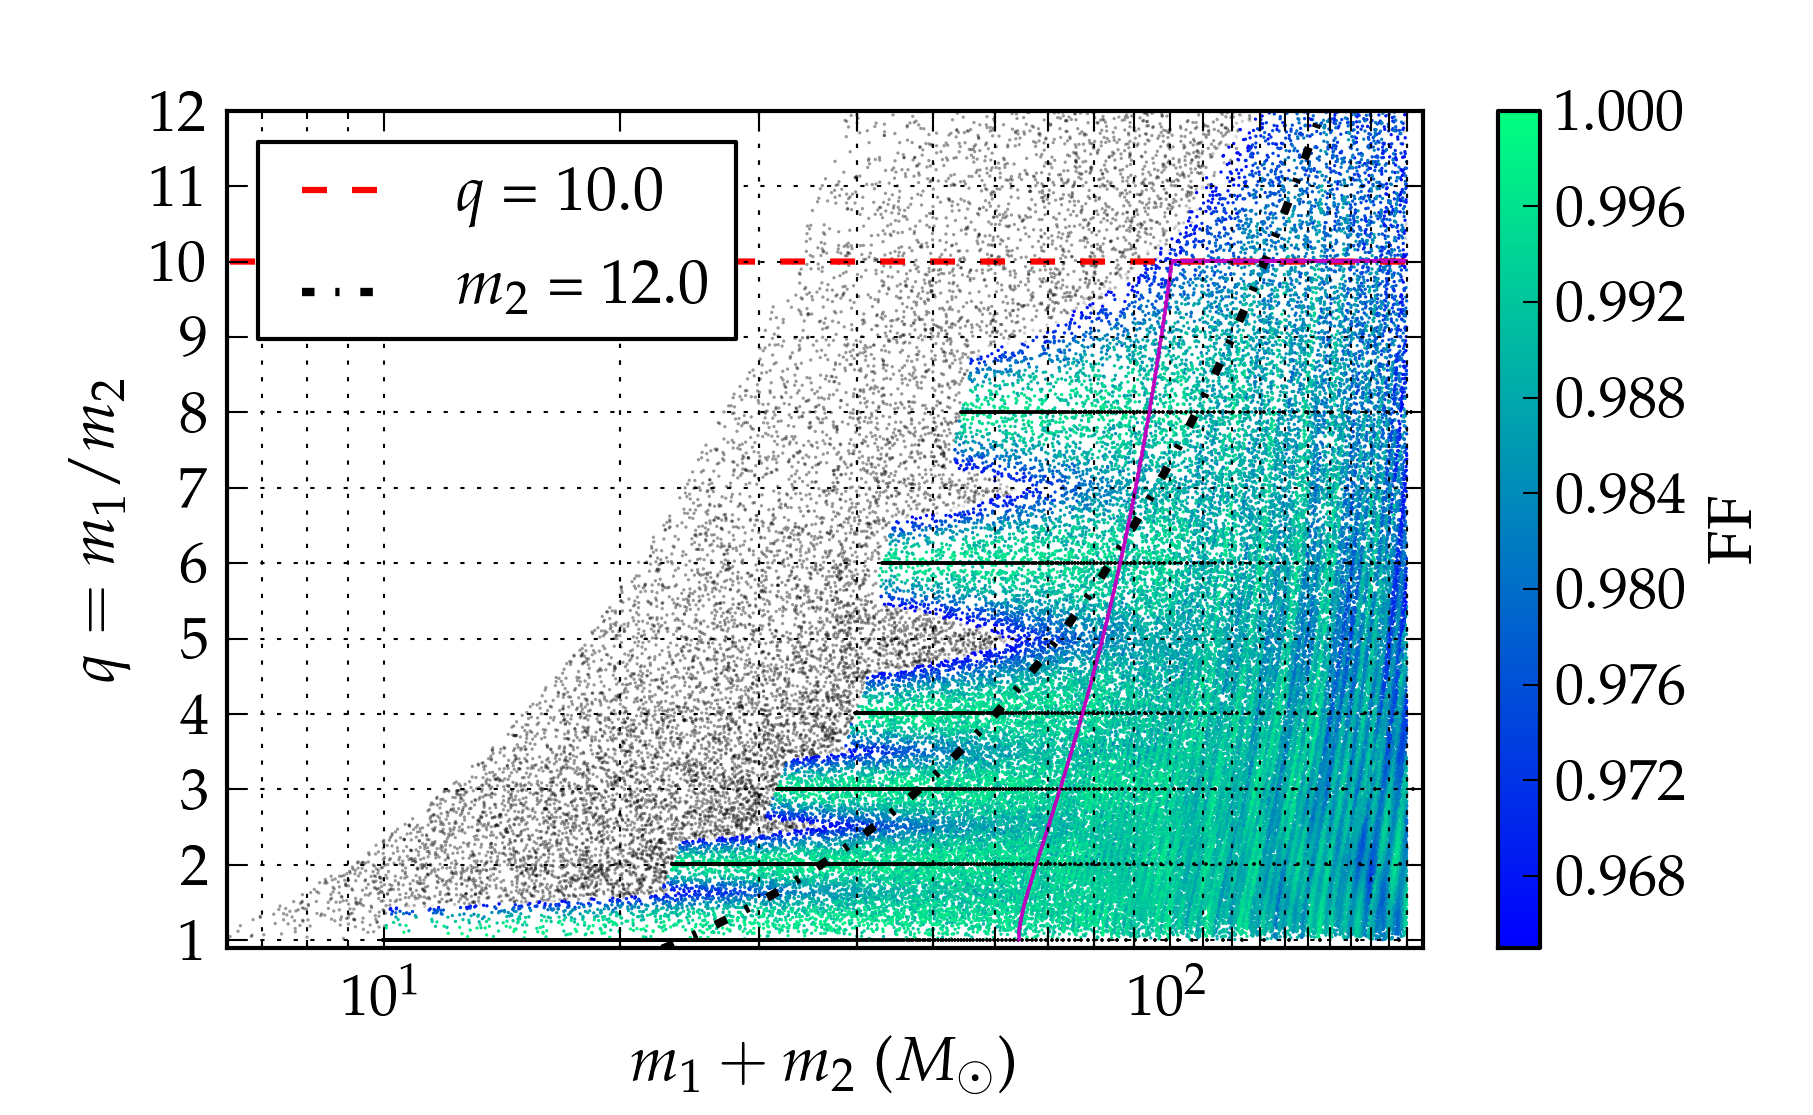
\includegraphics[width=\columnwidth]{bank_26022013_02_mtot200_logMq_NOhybMM.png}
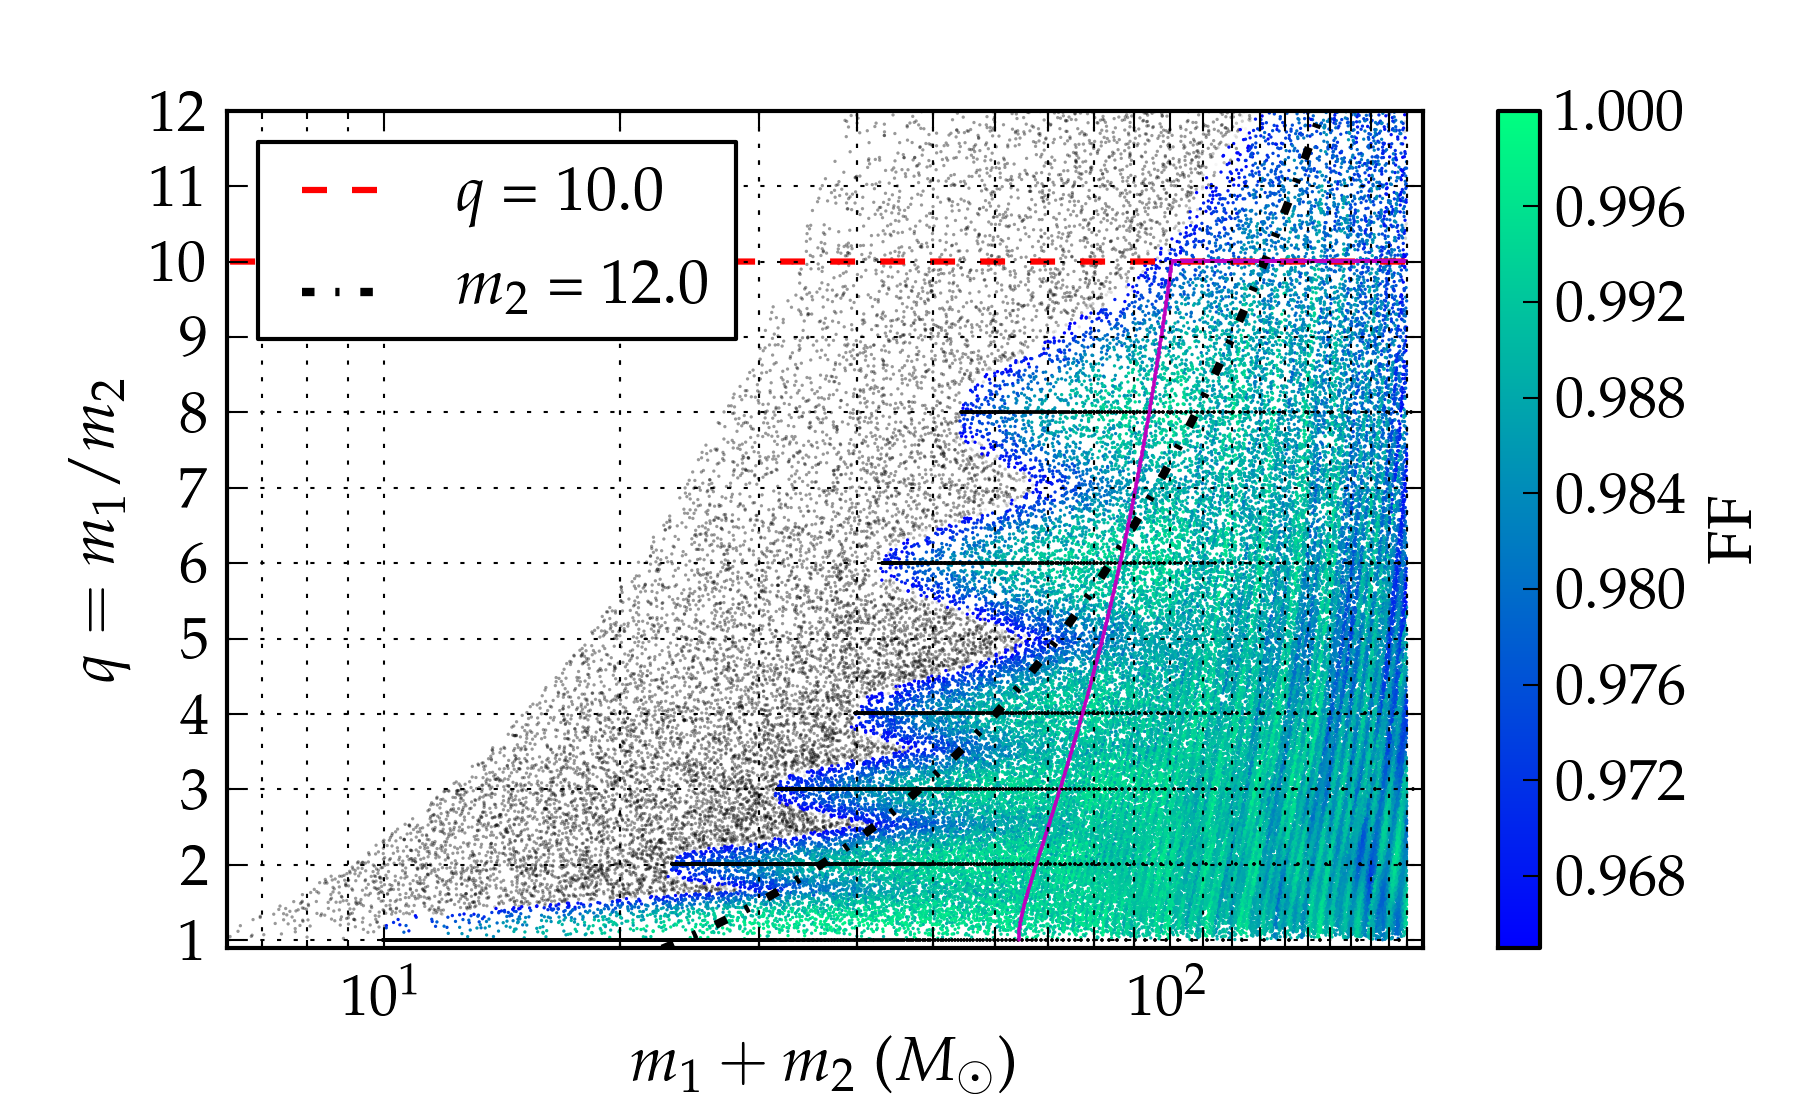
\includegraphics[width=\columnwidth]{bank_26022013_02_mtot200_logMq_hybMM.png}
\caption{\label{fig:Current-hybrids-FF}These figures are similar to 
  Fig.~\ref{fig:Current-hybrids-stochastic-FF}. The figures show fitting
  factors $\FF$ obtained when using a discrete mass-ratio template bank for
  $q=1,2,3,4,6,8$. For each mass-ratio, the templates are extended down 
  to a total mass where the NR-PN hybridization mismatch becomes
  $3\%$. Templates are placed independently for each mass-ratio, and span the 
  full range of total masses. For each mass-ratio, neighboring templates are 
  required to have an overlap of $97\%$. The union of the six single-$q$ 
  one-dimensional banks is taken as the final bank. The black dots show the 
  location of the templates. The fitting factor on the left plot does 
  {\em not} take into account the hybridization error, and therefore shows the
  effect of the sparse placement of the templates alone. The right plot accounts
  for the hybridization error
  and gives the actual fraction of the optimal SNR that would be recovered
  with this bank of NR-PN hybrid templates. The region bounded by the magenta 
  (solid) line in both plots indicates the lower end of the coverage of the 
  bank of un-hybridized NR waveforms. Lastly, the shaded grey dots show the 
  points where the fitting factor was below $96.5\%$.}
\end{center}
\end{figure*}

\begin{figure*}
\begin{center}
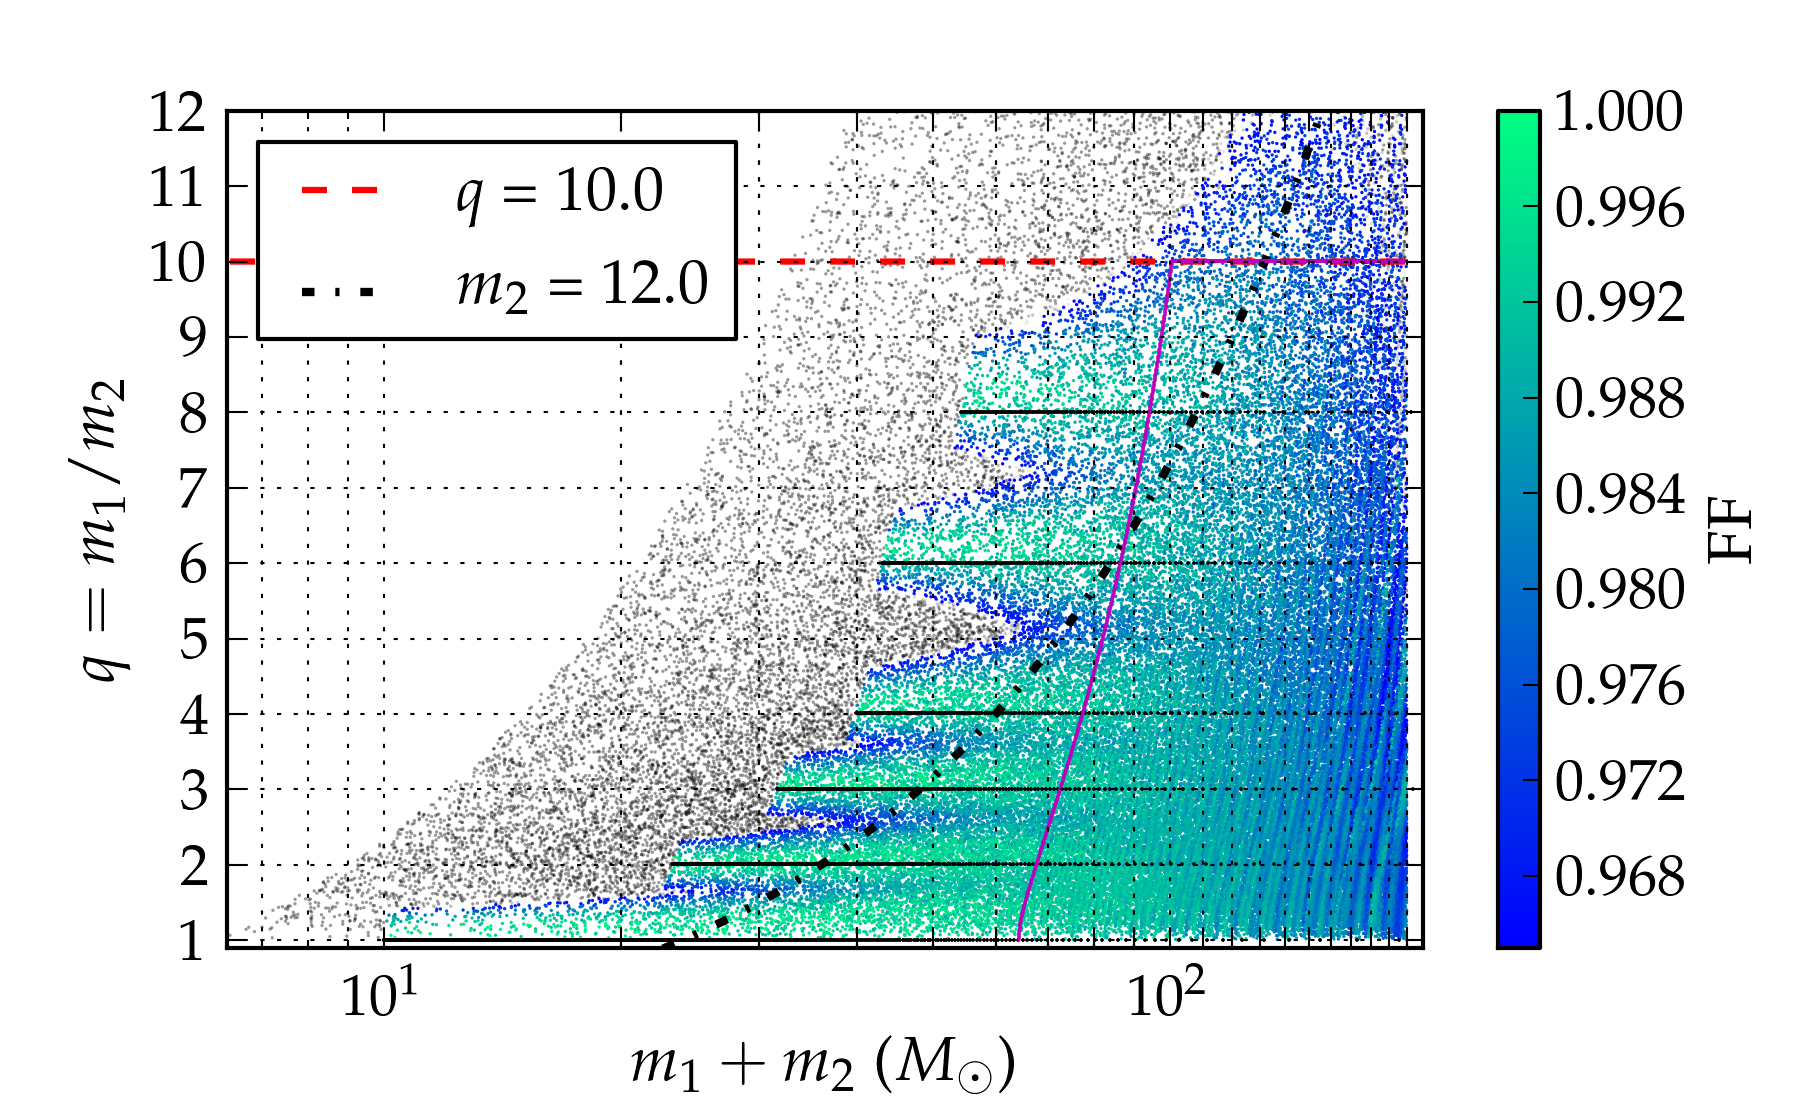
\includegraphics[width=\columnwidth]{bank_26022013_02_hybrids_mtot200_logMq_NOhybMM.png}
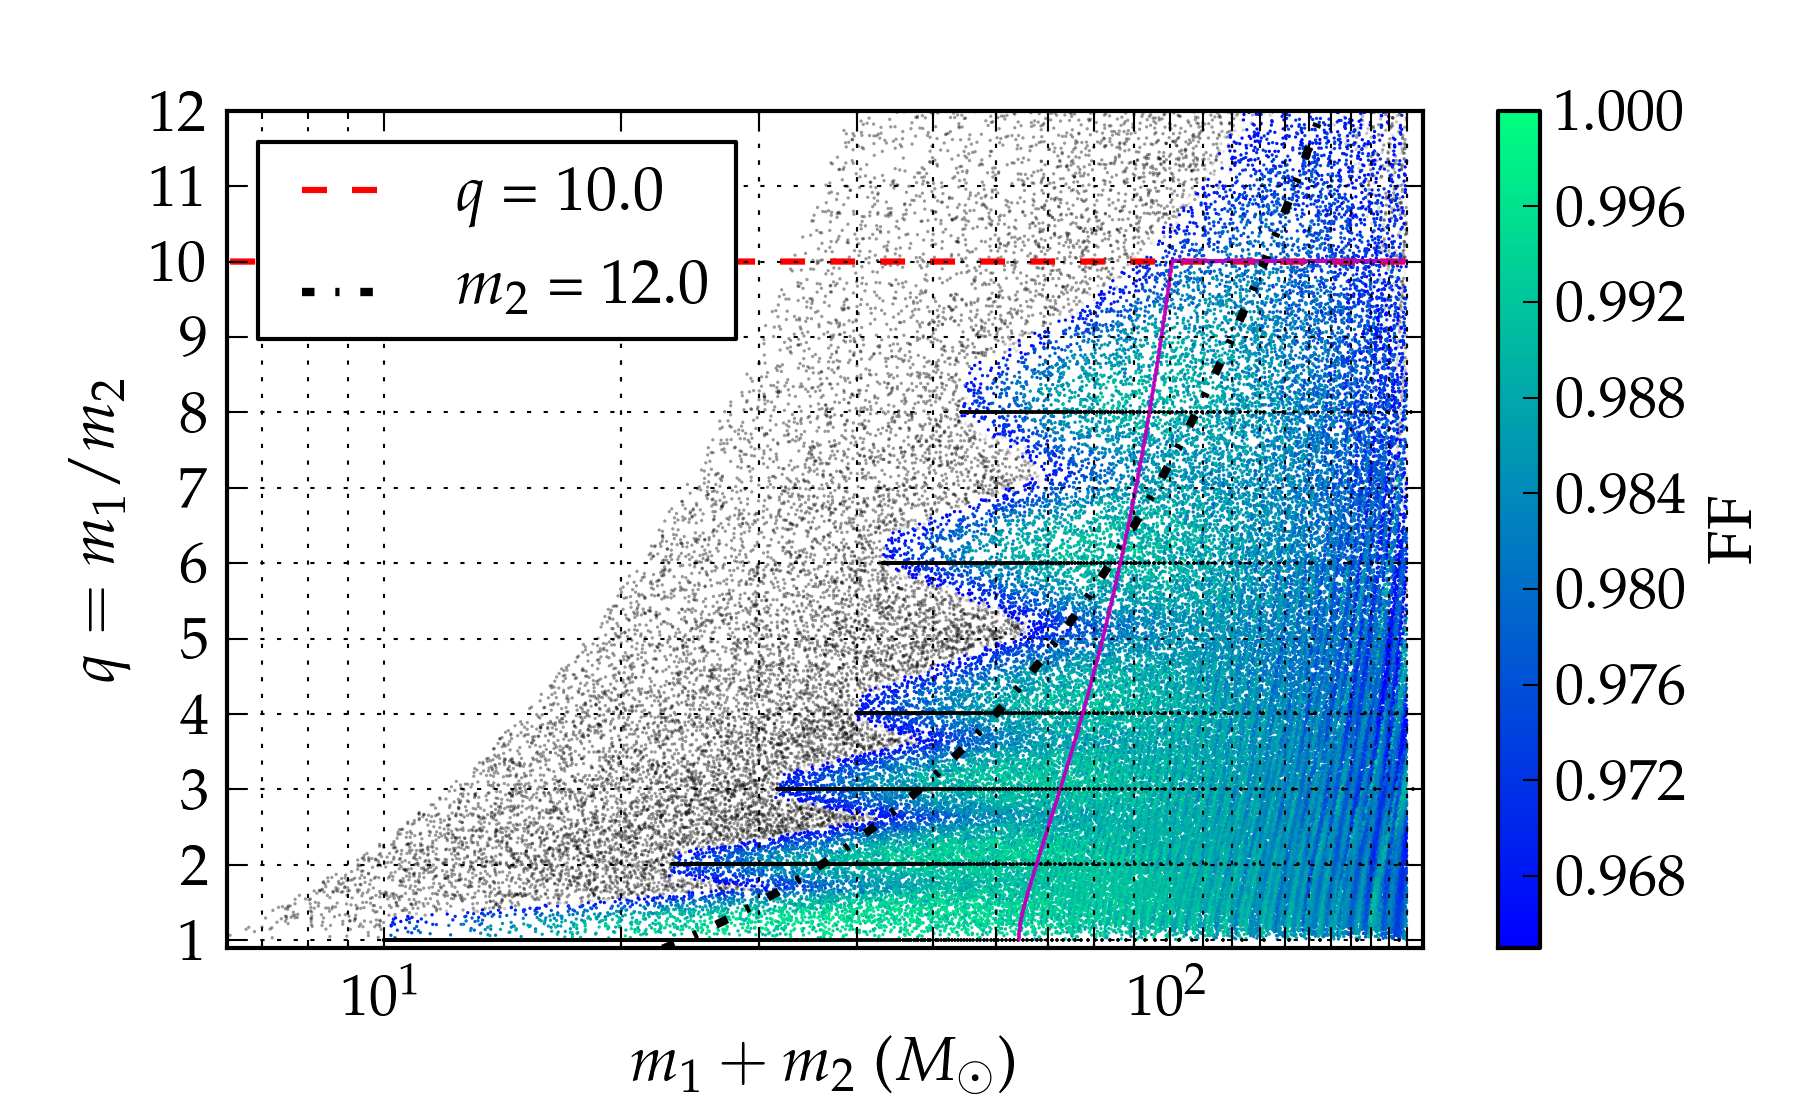
\includegraphics[width=\columnwidth]{bank_26022013_02_hybrids_mtot200_logMq_hybMM.png}
\caption{\label{fig:Current-real-hybrids-FF}This figure is similar to 
  Fig.~\ref{fig:Current-hybrids-FF}. The figures show fitting
  factors $\FF$ obtained when using a discrete mass-ratio template bank for
  $q=1,2,3,4,6,8$. Templates are placed independently for each mass-ratio, and 
  span the range of total masses, down to the region where the hybrid errors
  become $3\%$. For each mass-ratio, neighboring templates are 
  required to have an overlap of $97\%$. The union of the six single-$q$ 
  one-dimensional banks is taken as the final bank. The black dots show the 
  location of the templates. The GW signals are modeled using the EOBNRv2
  approximant~\cite{BuonannoEOBv2Main}, while TaylorT4+NR hybrids are used as
  templates. The fitting factor on the left plot shows the combined effect of 
  the sparse placement of the templates, and the (relatively small) 
  disagreement between the hybrid and EOBNRv2 waveforms. The right plot
  explicitly accounts for the hybridization error and gives the (conservative)
  actual fraction of the optimal SNR that would be recovered
  with this bank of NR-PN hybrid templates. The region bounded by the magenta 
  (solid) line in both plots indicates the lower end of the coverage of the 
  bank of un-hybridized NR waveforms. Lastly, the shaded grey dots show the 
  points where the fitting factor was below $96.5\%$.  }
\end{center}
\end{figure*}

%\textcolor{red}{How do we construct the stochastic bank, and how well does it perform?}\newline
We now consider template banks viable for hybrids constructed from currently 
available NR waveforms at mass ratios $q=1,2,3,4,6,8$. The lower mass limit,
in this case, is extended down to masses where the hybridization error 
exceeds $3\%$. We demonstrate two independent methods of laying
down the bank grid. First, we use the stochastic placement method that proceeds
as described in Sec.~\ref{s1:NRonlybank}. The templates are sampled over the
total mass - mass-rato $(M,q)$ coordinates, sampling $q$ from the restricted
set. The total mass $M$ is sampled from the continuous interval between the 
lower mass limit, which is different for each $q$, and the upper limit of
$200M_\odot$. To assess the SNR loss from the sparse placement
of the templates, we simulate a population of $100,000$ BBH signal waveforms,
with masses sampled with $3M_\odot\leq m_{1,2}\leq 200M_\odot$ and 
$M\leq 200M_\odot$, and filter them through the bank. This portion of the SNR
loss needs to be measured with both signals and templates in the same waveform
manifold. We use the EOBNRv2 approximant~\cite{BuonannoEOBv2Main} to model both, 
as it has been calibrated to most of the NR waveforms we consider here, and it
allows us to model waveforms for arbitrary systems. The left panel of
Fig.~\ref{fig:Current-hybrids-stochastic-FF} shows the
fraction of the optimal SNR that the bank recovers, accounting for its 
discreteness alone. We observe that, with just six mass-ratios, the bank 
can be extended to much lower masses before it is limited by the restricted
sampling of mass-ratios for the templates. For binaries with both black-holes 
more massive than $\sim 12M_\odot$, the spacing between mass-ratios was found 
to be sufficiently dense. The total SNR loss, after subtracting out 
the hybrid mismatches from Fig.~\ref{fig:Current-NR-PN-Errors}, are shown in 
the right panel of Fig.~\ref{fig:Current-hybrids-stochastic-FF}. 
At the lowest masses, the coverage shrinks between the lines of constant $q$ 
over which the templates are placed, due to the hybrid errors increasing 
sharply. We conclude that this bank is viable for hybrid templates for GW 
searches for BBHs with $m_{1,2}\geq 12M_\odot$, $1\leq q\leq 10$, and 
$M\leq 200M_\odot$. Over this region the bank will recover more than $96.5\%$
of the optimal SNR. This is a significant increase over the coverage allowed 
for with the purely-NR bank, the region of coverage of which is shown in the 
right panel of Fig.~\ref{fig:Current-hybrids-FF}, bounded at lowest masses by 
the magenta (solid) curve.


%\textcolor{red}{What is the second method, why do we use it, and how well does it compare?}\newline
Second, we demonstrate a non-stochastic algorithm of bank placement, with 
comparable results. We first construct six independent bank grids, each
restricted to one of the mass-ratios $q=1,2,3,4,6,8$, and spanning the full 
range of total masses. The spacing between neighboring templates is
given by requiring that the overlap between them be $97\%$. 
We take the union of these banks as the final 
two-dimensional bank. As before, we measure the SNR loss due to discreteness of
the bank and the waveform errors in the templates separately. To estimate the
former, we simulate a population of $100,000$ BBH systems, and filter
them through the bank. The signals and the templates are both modeled
with the EOBNRv2 model. The left panel of Fig.~\ref{fig:Current-hybrids-FF}
reveals the fraction of SNR recovered over the mass space, accounting for the 
sparsity of the bank alone, i.e. $1-\Gamma_\mathrm{bank}$. At lower masses, 
we again start to see gaps between the lines of constant mass ratio which become
significant at $m_{1,2} \leq 12M_\odot$. 
The right panel of Fig.~\ref{fig:Current-hybrids-FF} shows the final fraction 
of the optimal SNR recovered, i.e. the $\FF$ as defined in Eq.~(\ref{eq:FFGammas}). 
As before, these are computed by subtracting out the hybrid mismatches 
$\Gamma_\Hyb$ in addition to the discrete mismatches, as described in
Sec.~\ref{s1:quantifyingerrors}. 

The efficacy of both methods of template bank construction
can be compared from Fig.~\ref{fig:Current-hybrids-stochastic-FF} and 
Fig.~\ref{fig:Current-hybrids-FF}. We observe that the final banks from either
of the algorithms have very similar SNR recovery, and are both effectual over
the range of masses we consider here. Both were also found to give a very 
similar number of templates. The uniform-in-overlap method yields a grid 
with $2,325$ templates. The stochastic bank, on the other hand, was placed with a
requirement of $98\%$ minimal mismatch, and had $2,457$ templates. 
This however includes templates with $m_{1,2} < 12M_\odot$. Restricted
to provide coverage over the region with $m_{1,2}\geq 12M_\odot$, $1\leq q\leq 10$,
and $M\leq 200M_\odot$, the two methods yield banks with $627$ and $667$
templates respectively. The size of these banks is comparable to one 
constructed using the second-order post-Newtonian TaylorF2 hexagonal 
template placement method~\cite{SathyaBankPlacementTauN,BabaketalBankPlacement,
SathyaMetric2PN,Cokelaer:2007kx}, 
which yields a grid of $522$ and $736$ templates, for a minimal
match of $97\%$ and $98\%$, respectively.

%\textcolor{red}{How do we show the robustness of the banks using NR hybrids?}\newline
Finally, we test the robustness of these results using TaylorT4+NR hybrids 
as templates. As before, we simulate a population of $100,000$ BBH signal 
waveforms. As we do not have hybrids for arbitary binary
masses, we model the signals as EOBNRv2 waveforms. This population is filtered
against a bank of hybrid templates. The SNR recovered is shown in the left 
panel of Fig.~\ref{fig:Current-real-hybrids-FF}. Comparing with the left panels 
of Fig.~\ref{fig:Current-hybrids-stochastic-FF},~\ref{fig:Current-hybrids-FF}, 
we find that the EOBNRv2 manifold is a reasonable approximation for the hybrid 
manifold; and that, at lower masses, there is a small systematic bias in the 
hybrids towards EOBNRv2 signals with slightly higher mass-ratios.
The right panel of Fig.~\ref{fig:Current-real-hybrids-FF} 
shows the fraction of optimal SNR recovered after subtracting out the hybrid
mismatches from the left panel. The similarity of the $\FF$ distribution between 
the right panels of Fig.~\ref{fig:Current-real-hybrids-FF} and 
Fig.~\ref{fig:Current-hybrids-stochastic-FF},~\ref{fig:Current-hybrids-FF}
is remarkable. This gives us confidence that the EOBNRv2 model is a good 
approximation for testing NR/hybrid template banks, as we do in this paper; 
and that a template bank of NR+PN hybrids is indeed effectual for binaries 
with $m_{1,2}\geq 12M_\odot$, $M\leq 200M_\odot$ and $q\leq 10$.




\subsection{Complete PN-NR hybrid bank for non-spinning BBH}\label{s2:futureNRpNhybridbank}

\begin{figure*}
\begin{center}
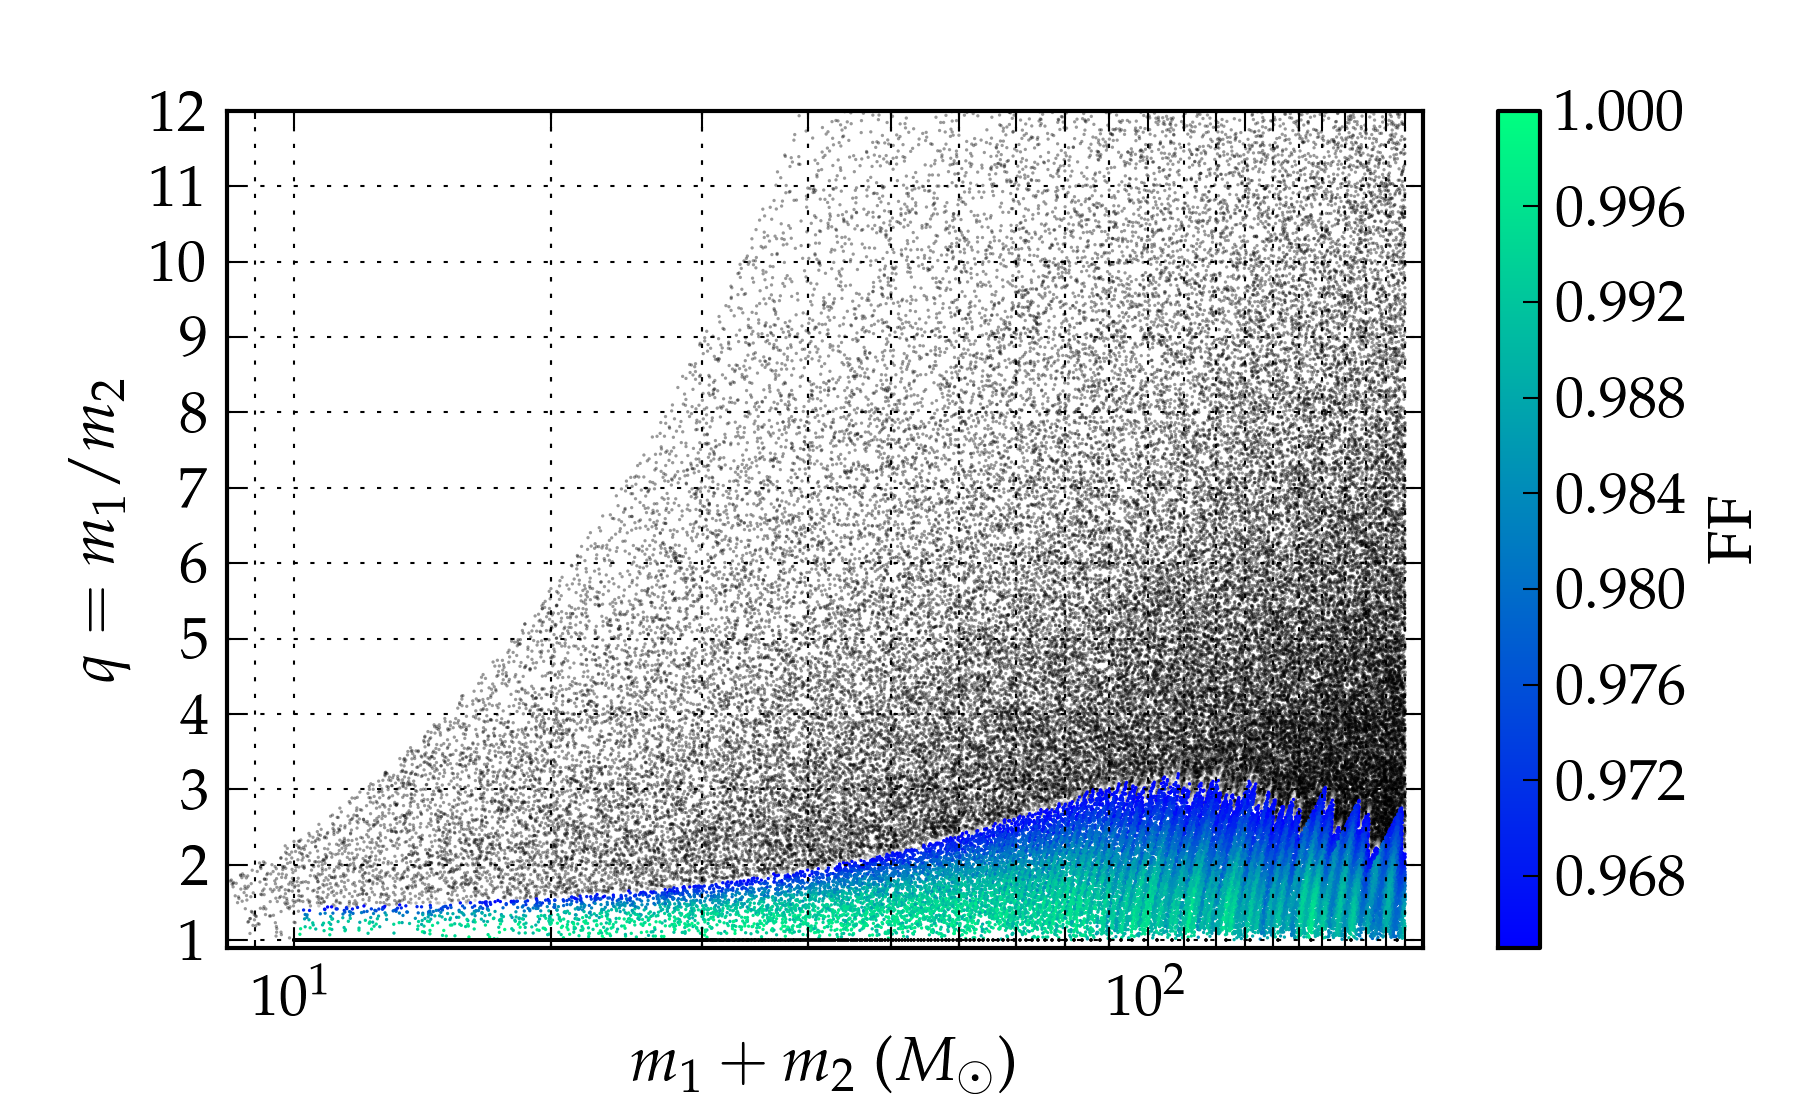
\includegraphics[width=0.33\textwidth, trim=17 20 75 40]{bank_separate_q1_mtot200_match.png}
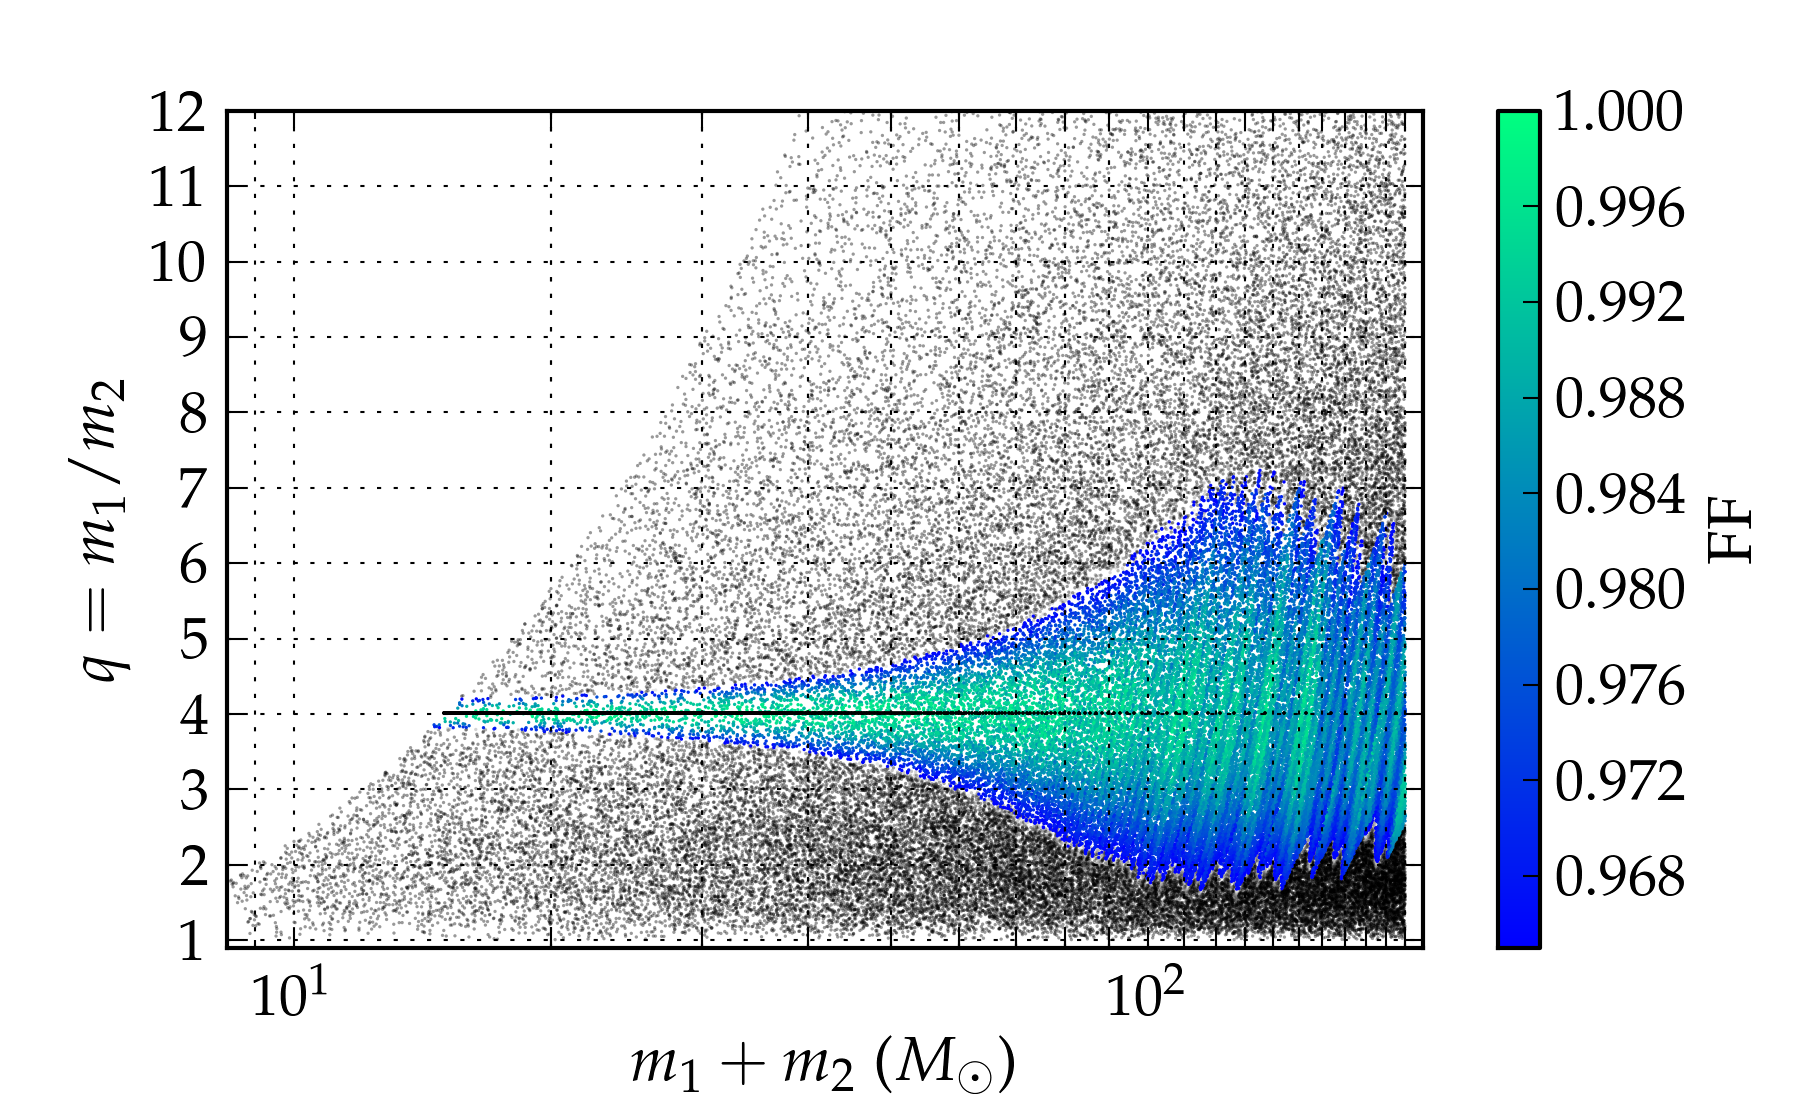
\includegraphics[width=0.33\textwidth, trim=17 20 75 40]{bank_separate_q4_mtot200_match.png}
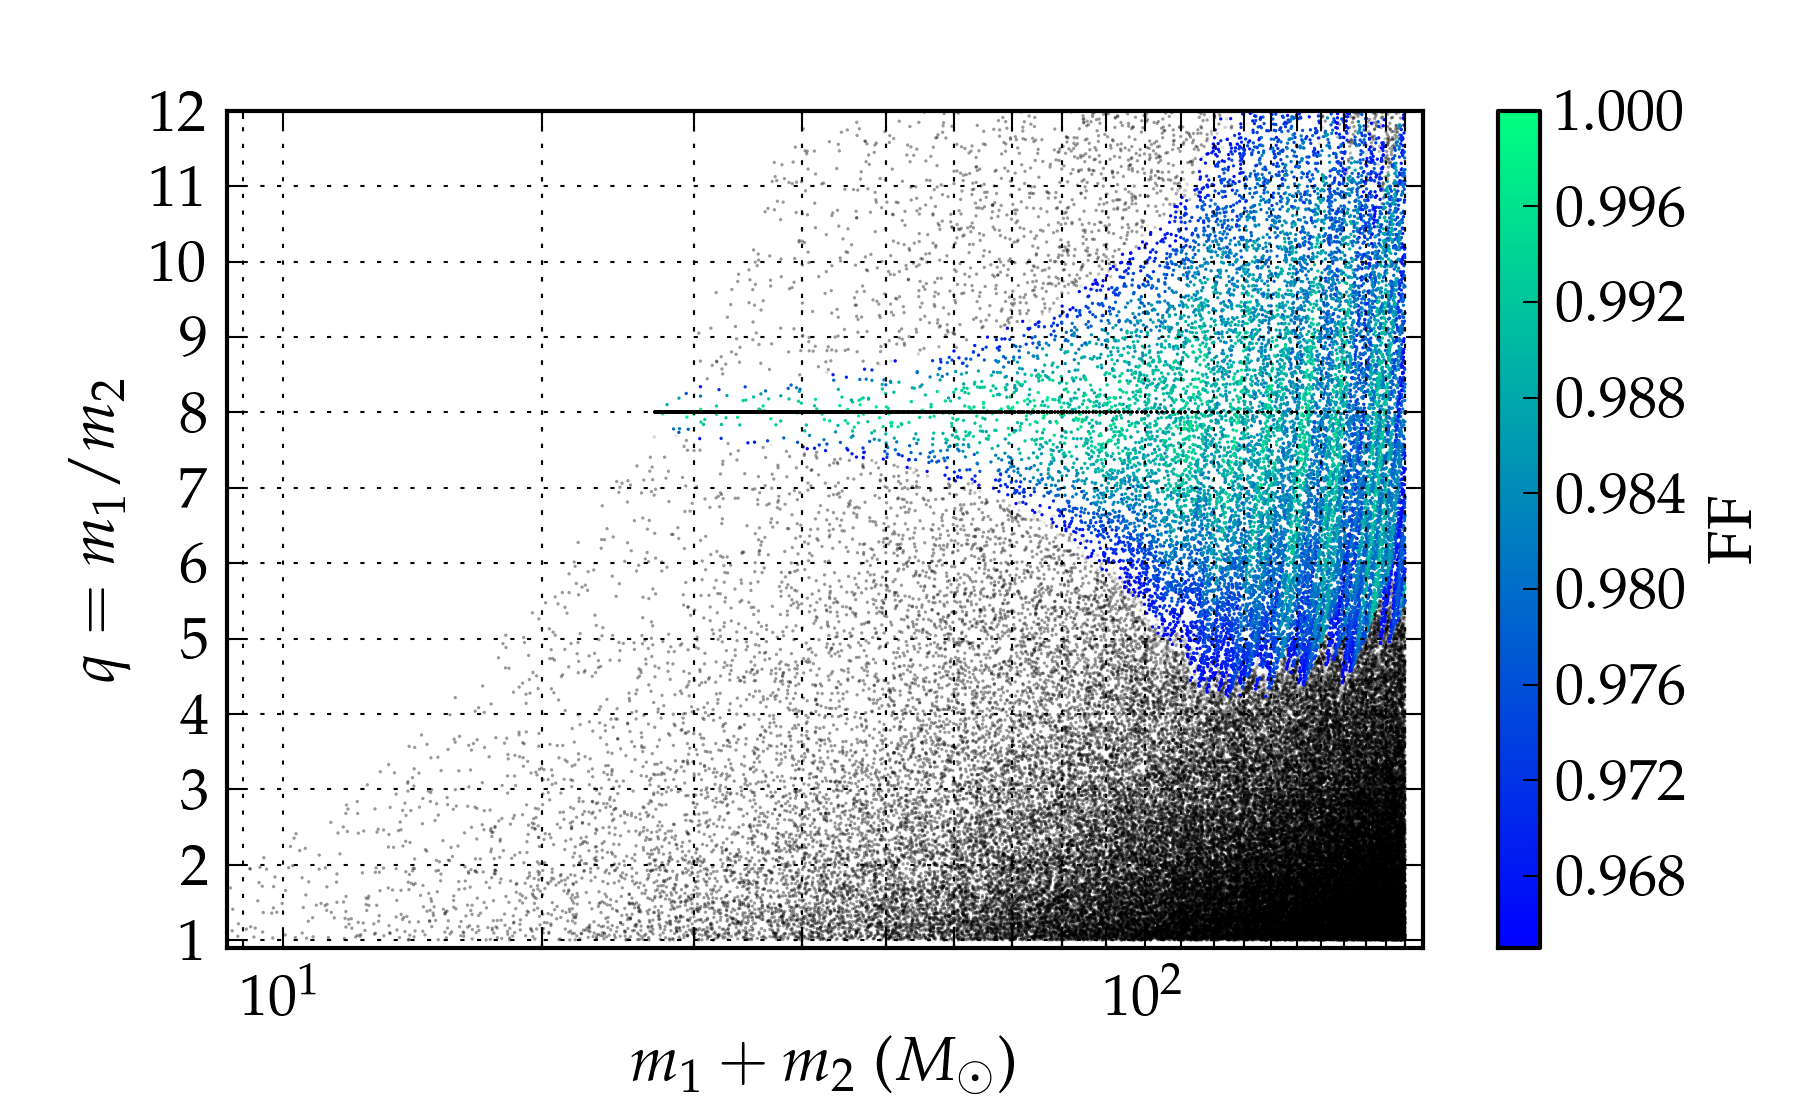
\includegraphics[width=0.33\textwidth, trim=17 20 75 40]{bank_separate_q8_mtot200_match.png}
\caption{\label{fig:separate_q148} These figures show the coverage of template
  banks restricted to single mass-ratios, i.e. (from left to right) 
  $q = 1, 4, 8$. We note that at 
  higher total masses, the templates are correlated to simulated signals for
  considerably different mass-ratios, than at lower total masses. This agrees
  with what we expect as with decreasing total mass, the number of cycles in
  the sensitive frequency band of Advanced LIGO increases.} 
\end{center}
\end{figure*}

%\textcolor{red}{Why do we need to extend the bank and where?}\newline
The last sections outlined properties of template banks of NR
waveforms (and their hybrids) which are available today. 
We also investigate the parameter and length requirements for future NR 
simulations, that would let us contruct detection template banks all the
way to $M=m_1+m_2=12M_\odot$. This lower limit was chosen following 
Ref.~\cite{Brown:2012nn,CompTemplates2009} which showed that the region with
$M\lesssim 12M_\odot$ can be covered with banks of post-Newtonian inspiral-only
waveforms.

%\textcolor{red}{Outline how we constructing the future-bank.}\newline
Constructing such a bank is a two-step process.  First, we pick mass-ratios 
that allow construction of such a bank given long enough waveforms for these
mass-ratios. Second, one needs to determine the necessary length of the NR 
portion of the waveforms, such that the PN-hybridization error is sufficiently
low for all masses of interest.

To motivate the first step, Fig.~\ref{fig:separate_q148} shows the coverage of
banks that sample from a {\em single} mass-ratio each (from left to right: $q=1,4,8$). We see that the resolution
in $q$ required at lower values of $M$ increases sharply below 
$M\sim 60M_\odot$. This follows from the increase in the number of waveform
cycles in aLIGO frequency band as the total mass decreases, which, in turn,
increases the discriminatory resolution of the matched-filter along the $q$ axis.
\begin{figure*}
\begin{center}
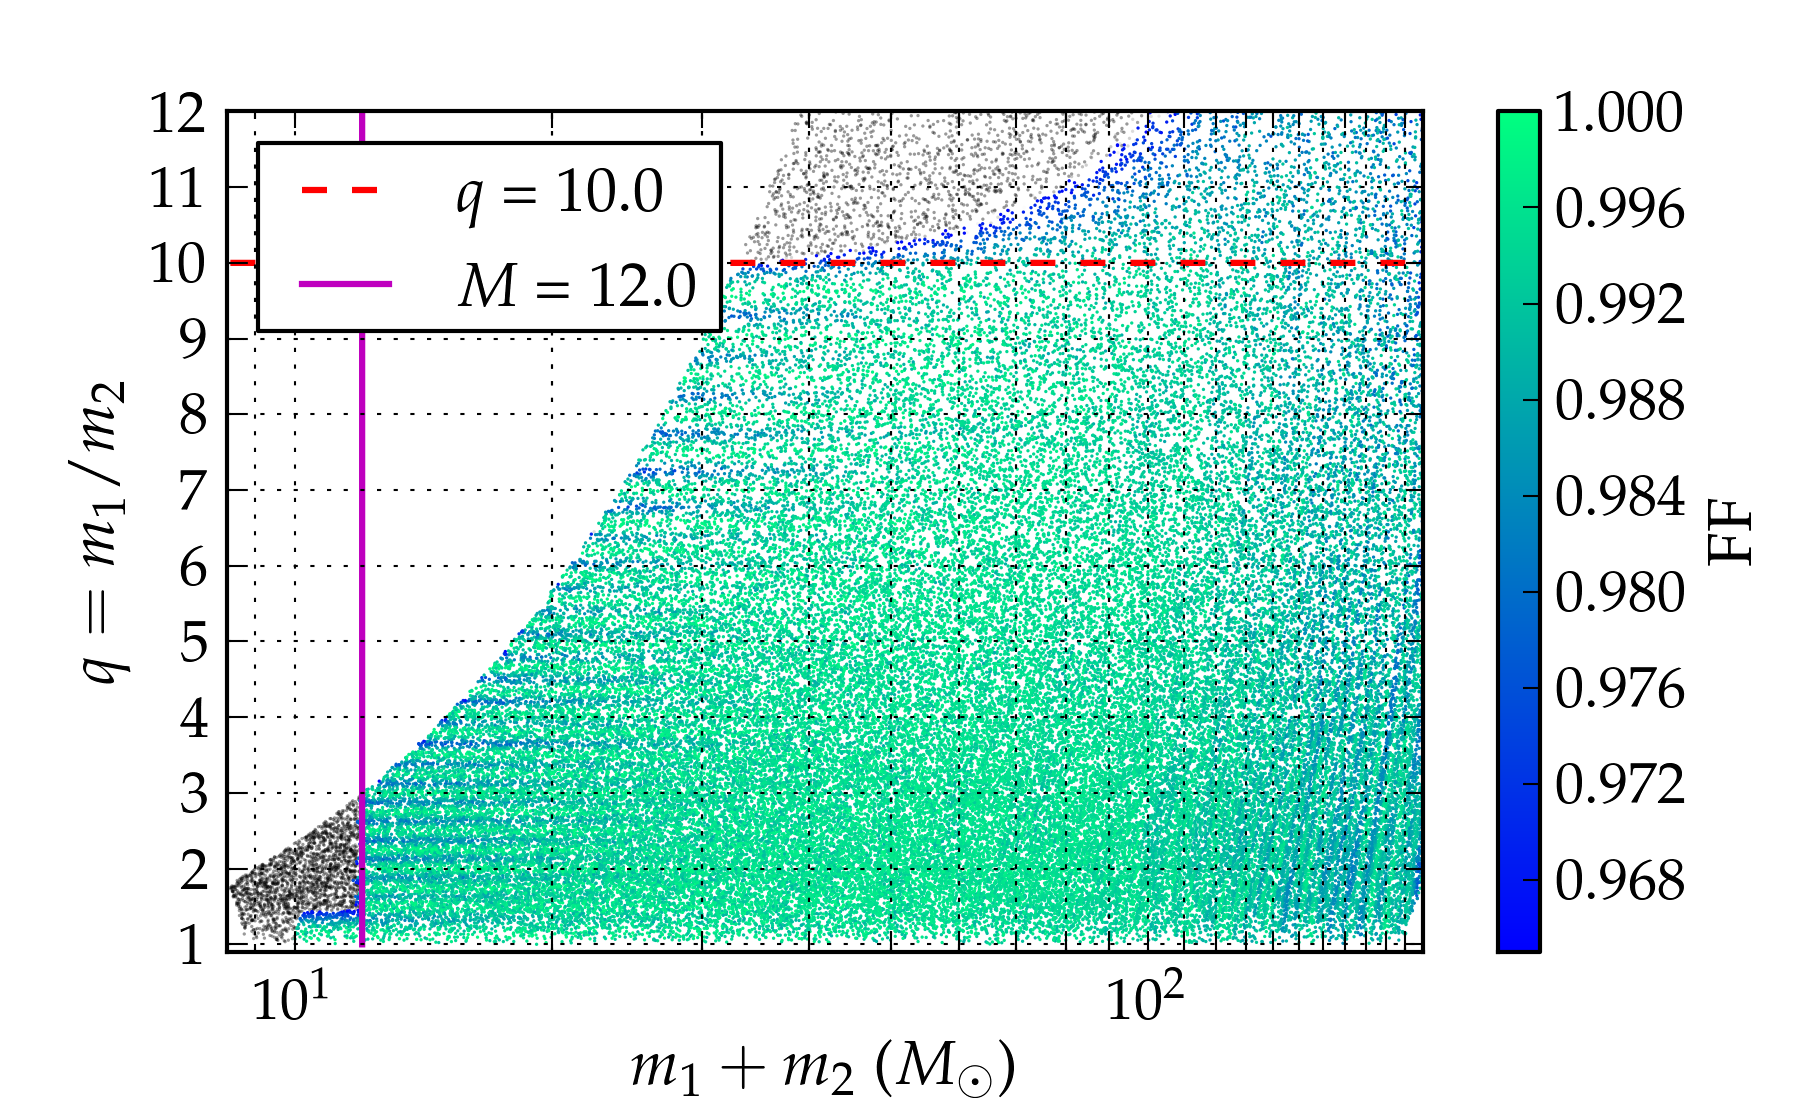
\includegraphics[width=\columnwidth]{bank_seperate_q1-4-35-4-65-9-6_01_mtot200_match.png}
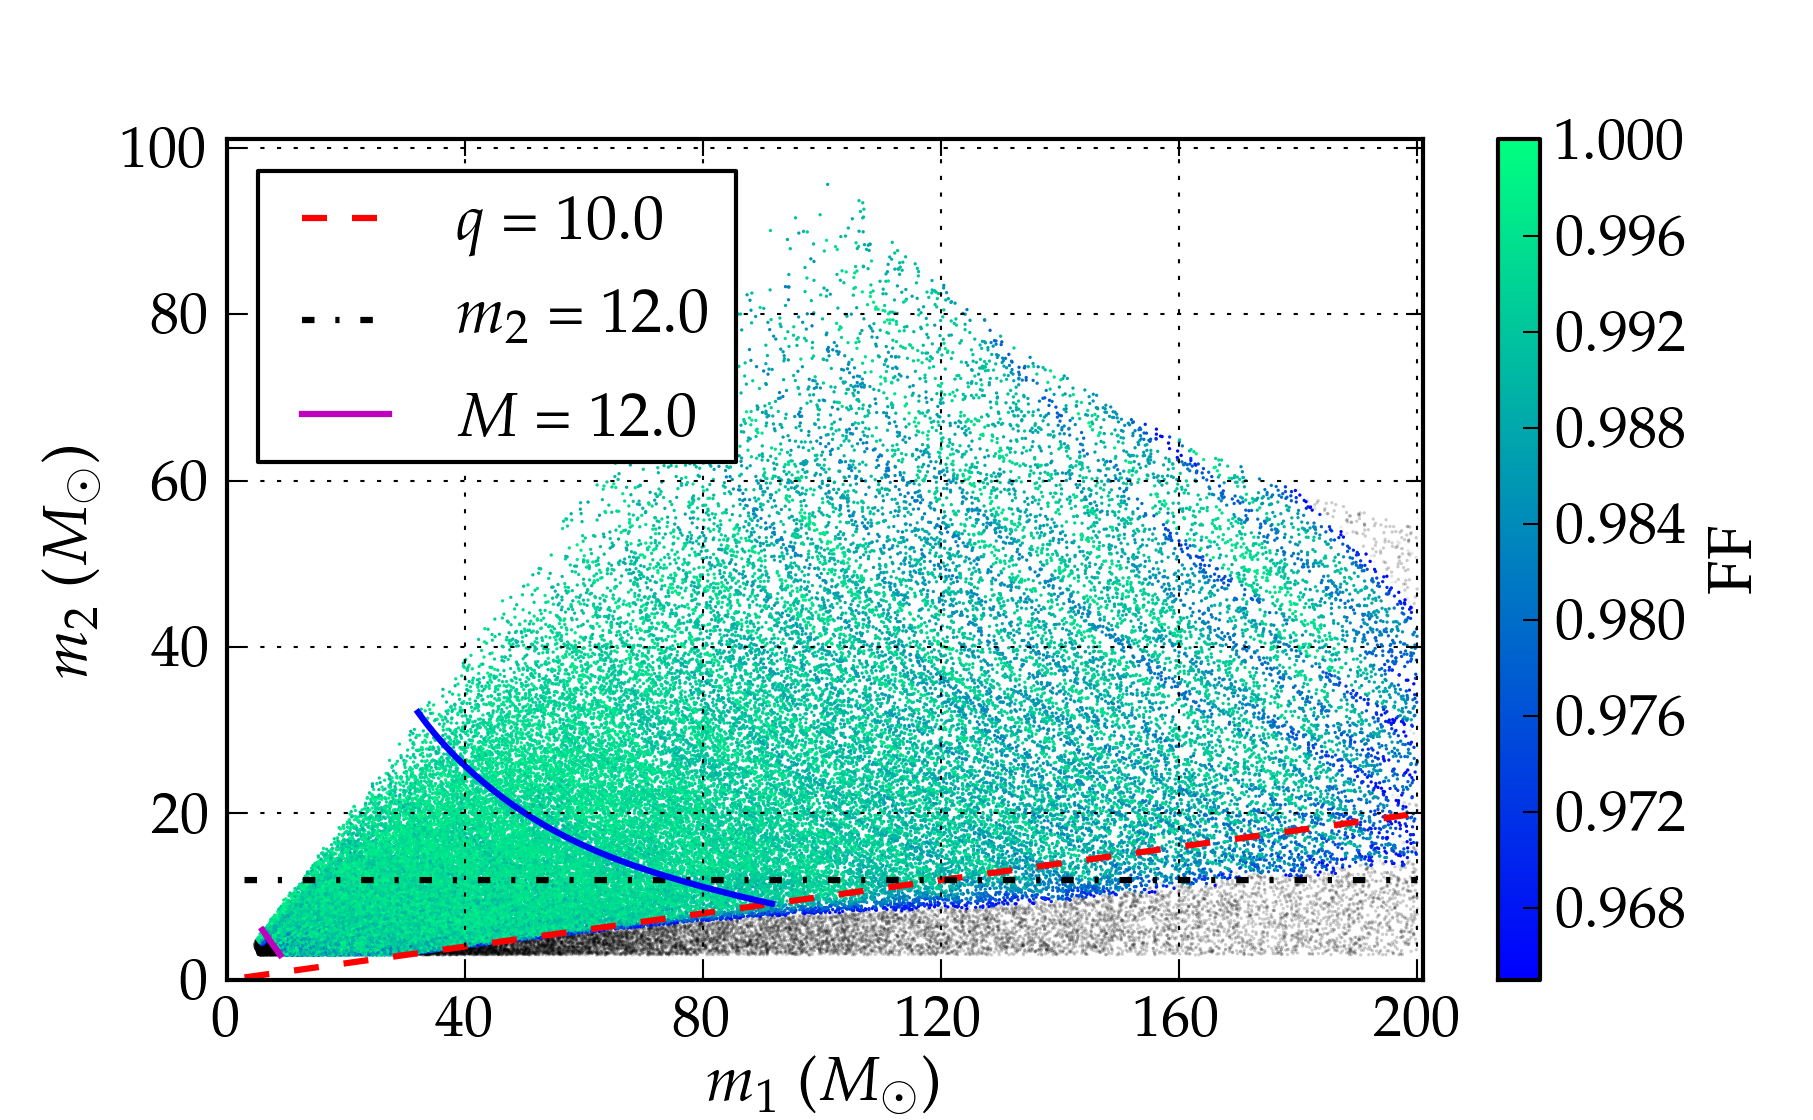
\includegraphics[width=\columnwidth]{bank_seperate_q1-4-35-4-65-9-6_01_m1m2200_match.png}
\caption{\label{fig:templatebank_halfMassRatios}This figure shows
  fitting factors for a hybrid template bank which samples from the 26 mass
  ratios $q=1,1.5,1.75,2,..,9.6$, and allows coverage to masses down to 
  $m_1 + m_2 = 12M_{\odot}$ and $1\leq q\leq 10$, with a minimal-match of $98\%$
  at the lowest masses. 
  The left and right panel show the same on $M-q$ and $m_1-m_2$ axes, 
  respectively. The magenta lines, in both panels, shows the upper bound 
  in total mass, below which frequency-domain PN waveforms can be used to construct template banks for aLIGO
  searches~\cite{CompTemplates2009,Brown:2012nn}. The dash-dotted line
  in the right panel shows the lower mass limit on the smaller component object,
  to which a bank of currently available NR-PN hybrids can cover, i.e.
  $\mn(m_1,m_2)=12M_\odot$ (see Sec.~\ref{s1:NRpNhybridbank}). The blue (solid)
  curve in  the right panel gives the lower mass limit to which a bank of
  currently available NR waveforms can cover (see Sec.~\ref{s1:NRonlybank}).
  Thus, between the simulations listed in Table~\ref{table:fullqlist}, 
  and frequency domain PN waveforms, we can search for the entire range of 
  BBH masses.}
\end{center}
\end{figure*}
\begin{table}
\begin{tabular}{| c |}
\hline
$q\,(\equiv m_1/m_2)$ \\ \hline
1, 1.5, 1.75, \\
2, 2.25, 2.5, 2.75, \\
3, 3.25, 3.5, 3.8, \\
4.05, 4.35, 4.65, 4.95, \\
5.25, 5.55, 5.85, \\
6.2, 6.55, \\
7, 7.5, \\
8, 8.5, \\
9, 9.6 \\
%0.0884 & 9.2 & ?? \\
\hline
\end{tabular}
\caption{List of mass-ratios, a template bank restricted to which will be effectual
over the region of the non-spinning BBH mass space where $m_1+m_2\gtrsim 12M_\odot$
and $1\leq q\leq 10$. The fraction of optimal SNR recovered by such a bank,
accounting for discreteness losses, remains above $98\%$. This is shown in
Fig.~\ref{fig:templatebank_halfMassRatios}.}
\label{table:fullqlist}
\end{table}
To determine the least set of mass-ratios which would sample the $q$ axis 
sufficiently densely at lower masses, we iteratively add mass-ratios to the 
allowed set and test banks restricted to sample from it. We find that, 
constrained to the set $\mathcal{S}_q$ given in Table~\ref{table:fullqlist},
%$=\{1, 1.5, 1.75, 2, 2.25, 2.5, 2.75, 3, 3.25, 3.5, 3.8, 4.05, 4.35,\\
%4.65, 4.95, 5.25, 5.55, 5.85, 6.2, 6.55, 7, 7.5, 8, 8.5, 9, 9.6\}$,
a template bank can be constructed that has a minimal match of $98\%$
at the lowest masses. The left panel of Fig.~\ref{fig:templatebank_halfMassRatios}
shows the loss in SNR due to bank grid coarseness, i.e. $1-\Gamma_\mathrm{bank}$. 
This loss remains below $2\%$ for mass-ratios $1\leq q\leq 10$, even at 
$M=12M_\odot$. This 
leaves a margin of $1.5\%$ for the hybrid mismatches that would incur due to 
the hybridization of the NR merger waveforms with long PN inspirals. The right 
panel of Fig.~\ref{fig:templatebank_halfMassRatios} shows the same data in the 
$m_1$-$m_2$ plane. In this figure, 
the region covered by the NR-only bank is above the blue (solid) curve, while 
that covered by a bank of the currently available NR-PN hybrids is above the
line of $m_2 = 12M_\odot$ (with $m_2\leq m_1$). The region from 
Ref.~\cite{Brown:2012nn,CompTemplates2009} that can be covered by PN templates 
is in the bottom
left corner, bounded by the magenta (solid) line. Our bank restricted to the
set of $26$ mass-ratios, as above, provides additional coverage for binaries
with $M\geq 12M_\odot$, $m_2\leq 12M_\odot$ and $1\leq q\leq 10$.
Thus between purely-PN and NR/NR-PN hybrid templates, we can construct 
effectual searches for non-spinning BBHs with $q\leq 10$.

\begin{figure*}
\begin{center}
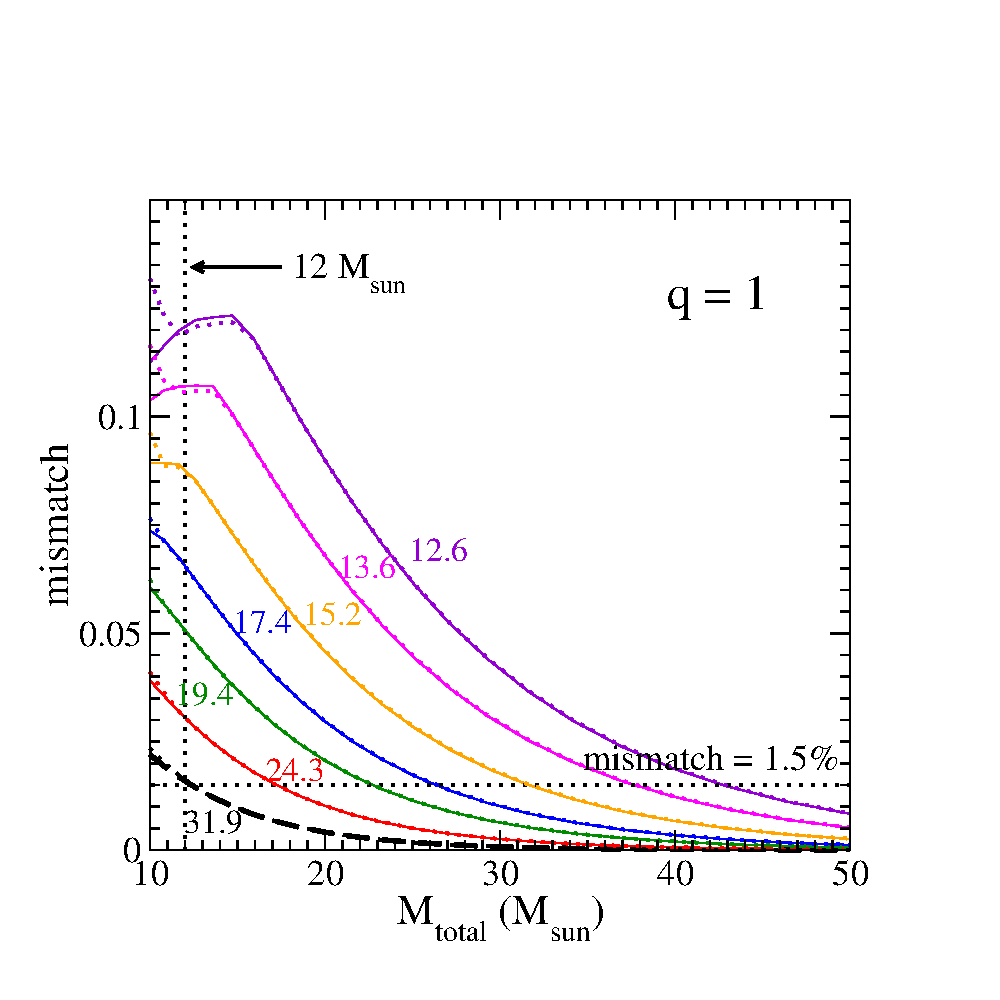
\includegraphics[width=0.33\textwidth, trim=17 20 75 75]{maxmismatchVSmass_q1.pdf}
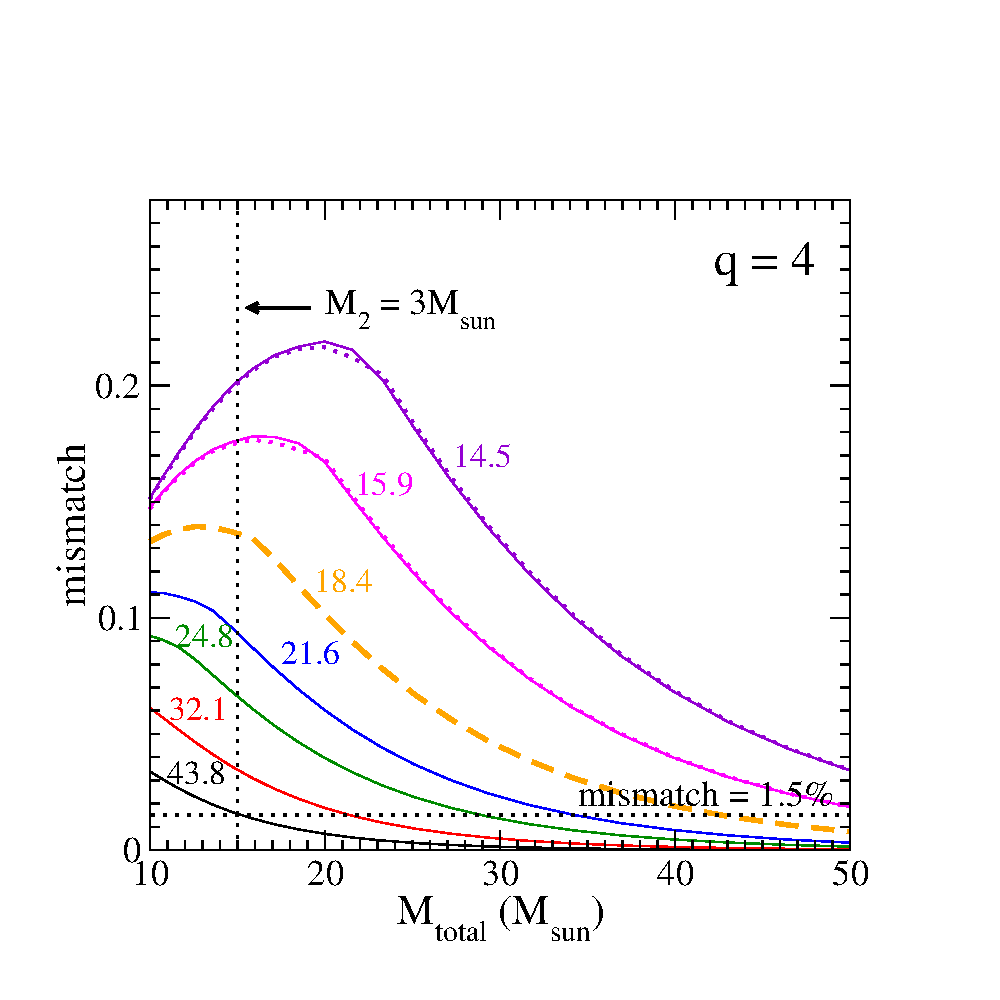
\includegraphics[width=0.33\textwidth, trim=17 20 75 75]{maxmismatchVSmass_q4.pdf}
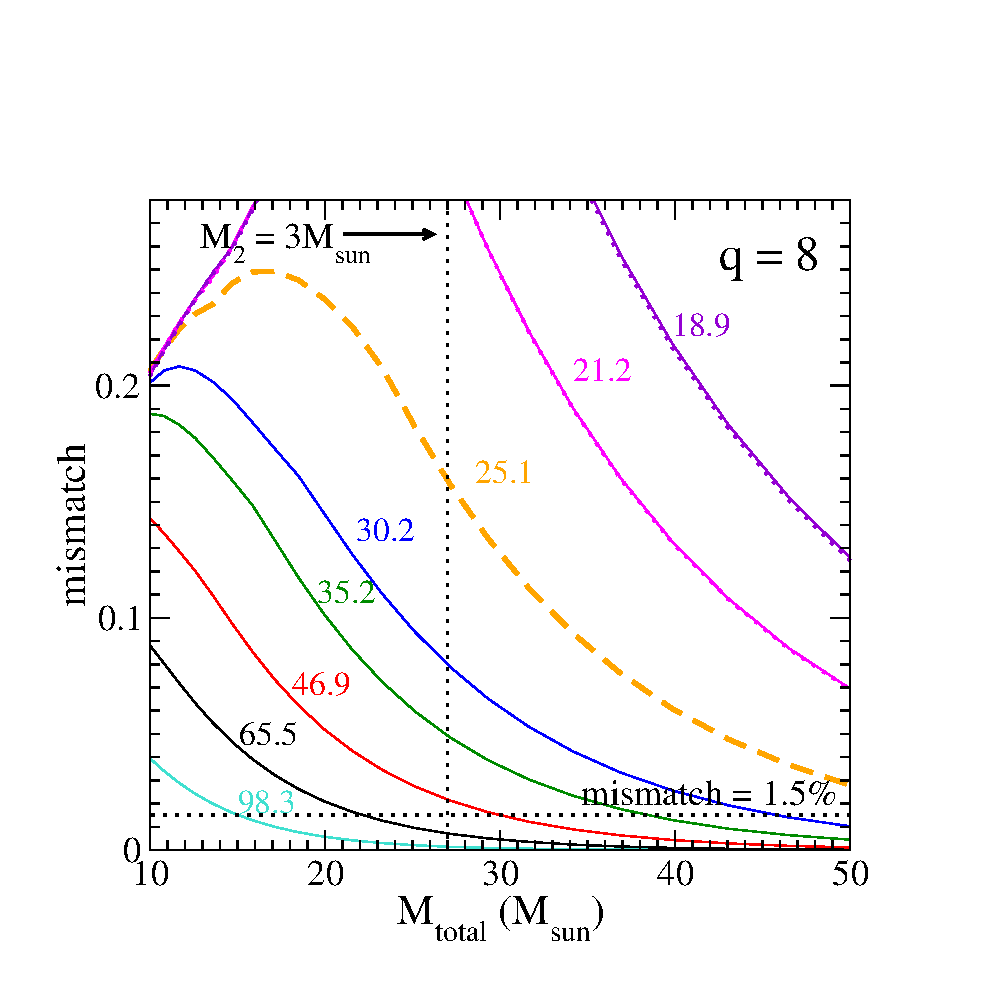
\includegraphics[width=0.33\textwidth, trim=17 20 75 75]{maxmismatchVSmass_q8.pdf}
\caption{\label{fig:maxmismatchVSmass} The maximum mismatch between
  different PN approximants for hybrid waveforms plotted against the
  total mass for at different matching frequencies ($M\omega_m$). The
  dotted lines indicate a mismatch of 1.5\% and a lower total mass
  limit, 12$M_\odot$ for $q=1$, and $M_2 = 3M_\odot$ for $q =
  4,8$. The thick dashed lines indicate the currently possible  
  matching frequency for hybrids based on the length of NR
  waveforms. The numbers next to each line indicate the number of
  orbits before merger where the PN and NR (or EOB) waveforms were 
  stitched together.} 
\end{center}
\end{figure*}

\begin{figure*}
\begin{center}
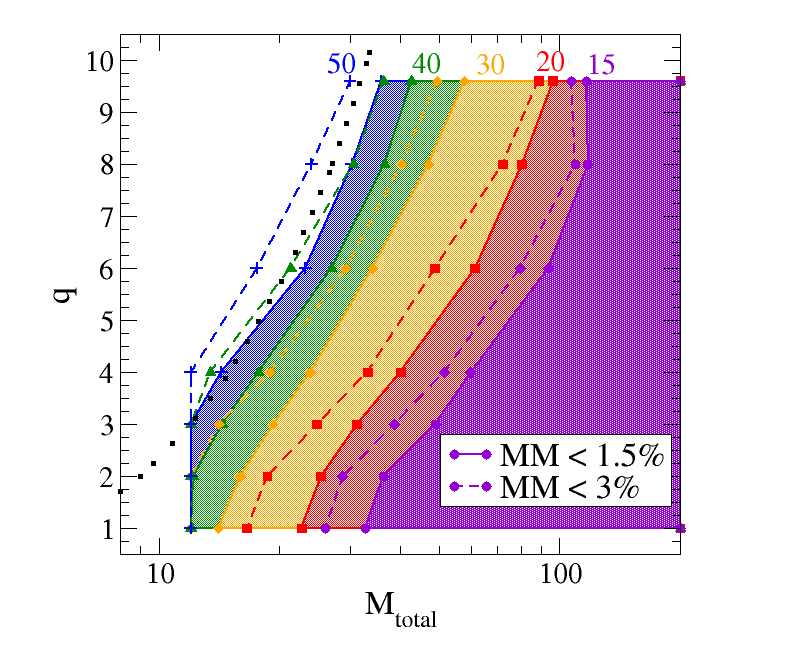
\includegraphics[width=\columnwidth, trim=17 25 75 25]{NRorbits2merger_cropped.png}
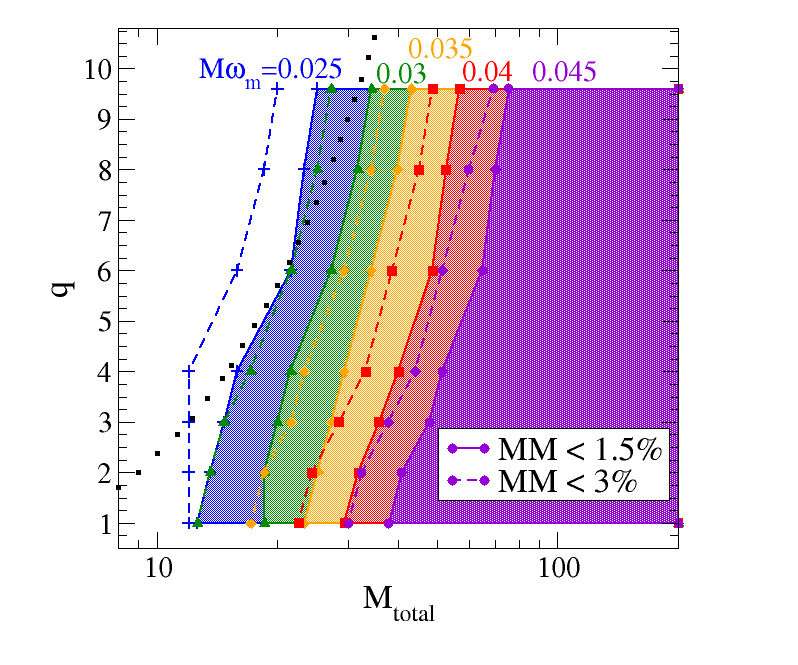
\includegraphics[width=\columnwidth, trim=17 25 75 25]{NRomega_cropped.png}
\caption{\label{fig:NRorbits2merger} This plot shows the lower mass limit
  of a template bank constructed with hybrid waveforms in terms of the
number of NR orbits (left panel) and initial gravitational wave
frequency (right panel) needed to have a PN error below $1.5\%$ (solid
curves) or $3\%$ (dashed curves). The dotted line indicates the
lower total mass limit when one component mass is $3M_\odot$.}
\end{center}
\end{figure*}

Having the set of required mass-ratios ${\cal S}_q$ determined, 
we need to decide on the length requirements for the NR simulations,
in order to control the PN hybridization error.  
For a series of matching frequencies, we construct
NR-PN hybrids with Taylor\{T1,T2,T3,T4\} inspirals, and compute their
pairwise mismatch as a function of total mass. The maximum of
these mismatches serves a conservative bound on the PN-hybridization 
error for that hybrid (c.f. Eq.~(\ref{eq:GammaHybfinal})).
Fig.~\ref{fig:maxmismatchVSmass} shows the results of this calculation.
Each panel of
Fig.~\ref{fig:maxmismatchVSmass} focuses on one mass-ratio. Within
each panel, each line represents one matching-frequency, with lines
moving down toward earlier hybridization with smaller mismatches.
Because the hybridization frequency is not particularly intuitive, the
lines are labeled by the number of orbits of the NR portion of the
hybrid-waveform. For a short number of orbits this calculation is
indeed done with NR waveforms, whereas for large number of orbits, we
substitute EOBNRv2 waveforms. The dashed lines represent the earliest
one can match a NR+PN hybrid given the currently available NR
waveforms, and are the same as the $q = 1,4, \text{ and } 8$ lines in
Fig~\ref{fig:Current-NR-PN-Errors}. The solid curves show the results
using EOB hybrids, while the dotted curves (just barely visible) show
the results with NR hybrids. They are virtually identical, which is a
confirmation that EOB hybrids can act as a good proxy for NR
hybrids in this case. The horizontal dotted line
indicates a mismatch of 1.5\%, while the vertical dotted line shows a
lower mass limit for each mass ratio: $12M_\odot$ for $q=1$, which is
the point at which one can construct a template bank with only PN
inspirals, $15M_\odot$ for $q = 4$, and $27M_\odot$ for $q =8$, which
are the lower mass limits if both component masses are $\geq 3M_\odot$. 

Fig.~\ref{fig:NRorbits2merger} presents the information obtained in
the previous paragraph in a different way.  Given NR-PN hybrids with
$N$ orbits of NR, the shaded areas in the left panel of Fig.~\ref{fig:NRorbits2merger}
indicate the region of parameter space for which such hybrids have
hybridization errors smaller than $1.5\%$.  As before, we see that for
high masses, comparatively few NR orbits are sufficient (e.g. the
purple $N=15$ region), whereas lower total masses require increasingly
more NR orbits. The dashed lines indicate the region of parameter
space with hybrid error below $3\%$. The black dotted line designates
the point where one component mass is greater than $3M_\odot$, which
is a reasonable lower mass limit for a physical black hole. The right
panel shows this same analysis instead with initial GW frequency
indicated by the solid and dashed lines. Thus, for the region of
parameter space we're interested in, no more than $\sim 
50$ NR orbits, or an initial GW frequency of $M\omega = 0.025$ would
be necessary to construct a detection bank with  hybrid mismatches
below $1.5\%$.  





%\FloatBarrier
\section{Conclusions}\label{s1:conclusions}
%%%%%%%%%%%%%%%%%%%%%%%%%%%%%%%%%%%%%%%%%%%%%%%%%%%%%%%%%%%%%%%%%%%%%%%%%%%%%%%
%%% Describe the wondrous conclusions of the thesis.
%%%%%%%%%%%%%%%%%%%%%%%%%%%%%%%%%%%%%%%%%%%%%%%%%%%%%%%%%%%%%%%%%%%%%%%%%%%%%%%

With the advent of Advanced LIGO and Advanced Virgo detectors, 
gravitational wave searches are expected to be able to see up to $10$
times further out in the universe, leading to a thousandfold increase in 
the volume of the accessible universe. Assuming a uniformly 
distributed population of compact object binaries in co-moving volume, 
we expect to see up to a three orders of magnitude increase in the detection 
rate. Gravitational wave searches make use of theoretical knowledge of
binary dynamics and employ modeled waveforms as filter templates.
With the increase in sensitivity, the resolution of the detectors 
for small errors in modeled waveforms also increases. In this dissertation,
we primarily focus on selecting and developing optimal waveform filters
for Advanced LIGO searches, as well as validating modeled search algorithms
using accurate simulated signals embedded in emulated detector noise.

For binaries with masses $m_1,m_2\leq 25M_\odot$, we compare the 
conventionally used post-Newtonian waveforms with the more recently 
developed Effective-One-Body (EOB) ones. As the EOB model is calibrated
against high-accuracy numerical simulations of non-spinning binary 
black holes, it is demonstrably an accurate model for {\it comparable}
mass-ratio binaries. However, it is computationally more expensive
than the post-Newtonian approximants. 
We investigate the region of the parameter
space of non-spinnning binaries where the accuracy of post-Newtonian
approximants is sufficient and we can win with computational cost, as
well as the region where EOB waveforms would be required. We also
study the impact of ignoring sub-dominant waveform multipoles in 
searches, and find that doing so decreases our ability to detect binaries
which have their orbital angular momentum highly inclined to the 
line of sight connecting them to terrestrial detectors.

More recently, very high accuracy fully numerical simulations of 
binary black holes have been performed, solving Einstein field equations
in full generality. While the methodology for performing such simulations
is being advanced at an accelerated pace, they are still expensive to 
perform for long durations of the coalescence process. However, hybrid
waveforms can be constructed where post-Newtonian approximants model the 
weak-field slow-motion portion and numerical relativity simulations 
model the strong-field fast-motion portion. We demonstrate that, within the 
limits of current numerical relativity technology, 
it is possible to use hybrid waveforms
in gravitational wave searches. Moreover, we show that this is possible in 
the entire region of the non-spinning binary parameter space where
post-Newtonian approximants are insufficient for Advanced LIGO searches.

Apart from having applications in enhancing the accuracy of theoretical 
and phenomenological waveform models, numerical simulations can also be used
to validate the gravitational wave search methods. We do precisely this within
the purview of the NINJA-2 project. Several numerical relativity groups contributed
post-Newtonian-hybridized simulations to the project. These were subsequently
injected in emulated advanced detector noise. We demonstrate the ability of
existing search algorithms to successfully {\it detect} these simulations
embedded within emulated noise. This is different from the NINJA-1 project
on a few counts, one of them being the nature of the emulated noise. In the 
NINJA-2 project, initial LIGO data with its non-Gaussian transient noise was
recolored to the expected sensitivity of the Advanced LIGO-Virgo detectors, as
opposed to colored Gaussian noise that was used in NINJA-1. 
Therefore this project provided a more robust test of our search methods, and 
provided a benchmark against which future search developments could be compared.


While the above concerns primarily comparable mass-ratio binaries, we 
also develop waveform models for intermediate mass-ratio ones with 
$m_1/m_2 \in [10, 100]$. First-order conservative self-force corrections 
have been derived for a test-particle moving in the background of a 
supermassive Schwarzschild black hole. Using the form of these calculations,
we develop a model to capture the inspiral dynamics of binaries with 
intermediate to extreme mass-ratios. Using this model, we are also able to 
estimate the orbital frequency at the inner-most stable circular orbit, 
for mass-ratios ranging from the comparable case to the test-particle limit.

Intermediate mass-ratio systems, containing intermediate mass and stellar
mass black holes will also be relatively more massive than stellar mass binaries.
This would shift the frequency of the emitted gravitational radiation to 
lower values, and their late-inspiral and merger would occur in the most
sensitive frequency band of Advanced detectors. This makes the modeling 
of the later portion of their waveforms crucial to their detection. 
We first reformulate the prescription to model the early and late inspiral
of such binaries. Then, using the implicit rotation source picture,
due to Baker et al~\cite{}, we develop a model for the plunge and merger
where the smaller object is no longer moving in quasi-circular orbits
and is very close to its partner. We then complete the description 
by stitching the quasi-normal ringdown waveform emitted by the black hole formed from 
the merger of the two initial holes. Therefore, we complete a model that
captures the entire coalescence process for intermediate mass-ratios.

To summarize, for {\it comparable} mass ratio binaries, we show that a combination
of post-Newtonian and post-Newtonian--Numerical-Relativity hybrid waveforms
would be sufficient for gravitational wave searches. This is true for the 
entire non-spinning binary black hole parameter space, up to arbitrarily high
masses. We also successfully validate gravitational wave search algorithms 
that have been used in the most recent LIGO-Virgo searches, using accurate 
numerical simulations injected in emulated detector noise. 
For {\it intermediate} mass ratios, we develop an accurate waveform 
model that captures the binary dynamics from the weak-field slow-motion
regime to the strong-field regime up to the merger of both compact objects. 
Therefore the work presented in this dissertation is an effort towards
arriving at optimal search filters for non-spinning binary black holes 
which are prospective sources detectable by the second-generation terrestrial
gravitational wave detectors; as well as towards validating existing search 
algorithms using an improved testing methodology.














\acknowledgments
We are grateful to the SXS collaboration. 

Part of the computations for the paper
were done on the

This work was supported by 
NSERC of Canada, the Canada Chairs Program, 
and the Canadian Institute for Advanced Research.

Simulations used in this work
were computed with the \texttt{SpEC} code~\cite{spec}.  Computations
were performed on the  SUGAR cluster, which is supported by \red{NSF grant PHY-XXXXX}; the Zwicky cluster at Caltech, which is supported by
the Sherman Fairchild Foundation and by NSF award PHY-0960291; on the
NSF XSEDE network under grant TG-PHY990007N; and on the GPC
supercomputer at the SciNet HPC Consortium~\cite{scinet}. SciNet is
funded by: the Canada Foundation for Innovation under the auspices of
Compute Canada; the Government of Ontario; Ontario Research
Fund--Research Excellence; and the University of Toronto.



\FloatBarrier
\bibliographystyle{apsrev4-1}
\bibliography{paper}

\end{document}
